% ==================================================================
%  徐森林、薛春华《数学分析》（第二册）
%  第 9 章  $n$ 元函数微分学的应用
%  源：印刷页 135 起 (PDF p. 141 起)
% ==================================================================

\chapter{\texorpdfstring{$n$}{n} 元函数微分学的应用}\label{ch:9}

第 8 章论述了 $n$ 元函数的 Taylor 公式与隐射、逆射定理. 作为隐射、逆射定理的应用, 在本章, 我们将研究 $C^{k}\,(k \geqslant 1)$ 参数曲面的切空间、法空间以及第一基本量; 证明条件极值的必要条件, 并给出了用 Lagrange 不定乘数法求条件极值. 9.2 节应用二次型
\[ Q(\boldsymbol{x}^{0}, \boldsymbol{t}) = \sum_{i, j=1}^{n}\frac{\partial^{2}f}{\partial x_{i}\partial x_{j}}(\boldsymbol{x}^{0})t_{i}t_{j} \]
描述了 $n$ 元函数在驻点处达到极值的充分条件, 它的证明正是 $n$ 元带 Lagrange 余项的 Taylor 公式的重要应用.

% ==================================================================
%  §9.1  曲面的参数表示、切空间
%  源：徐森林、薛春华《数学分析》第二册，印刷页 135-157 (PDF p. 141-163)
%  底本：PaddleOCR-VL-1.6 JSON/MD 识别结果，人工逐字核校与公式精修
%  插图：原生 TikZ 逐幅复刻（图 9.1.1 ~ 图 9.1.9）
%  规范：全西文标点，忠实原文定义、注、定理、例题、练习题编号与推导
% ==================================================================

\section{曲面的参数表示、切空间}\label{sec:9.1}

\begin{definition}\label{def:9.1.1}
设 $\Delta$ 为 $\mathbb{R}^{s}$ 中的开集,
\[
  \boldsymbol{x}\colon \Delta \to \mathbb{R}^{n}, \quad \boldsymbol{u} = (u_{1}, u_{2}, \cdots, u_{s}) \mapsto \boldsymbol{x}(\boldsymbol{u}) = (x_{1}(u_{1}, u_{2}, \cdots, u_{s}), \cdots, x_{n}(u_{1}, u_{2}, \cdots, u_{s}))
\]
为映射, 则称 $M = \boldsymbol{x}(\Delta) = \{\boldsymbol{x}(\boldsymbol{u}) \mid \boldsymbol{u} \in \Delta\}$ 为 $s$ 维曲面, 而 $\boldsymbol{x}(\boldsymbol{u})$ 又称为 $M$ 的参数表示. 当 $\boldsymbol{x}(\boldsymbol{u})$ 为 $C^{k}\,(k \geqslant 0)$ 时, 称 $\boldsymbol{x}$ 或 $M$ 为 $C^{k}$ 曲面.
\end{definition}

如果 $\boldsymbol{x}$ 是 $C^{k}\,(k \geqslant 1)$ 的, 则称 $\boldsymbol{x}$ 或 $M$ 为 $s$ 维 $C^{k}$ 光滑曲面. 当
\[
  \operatorname{rank}(\boldsymbol{x}_{u_{1}}^{\prime}(\boldsymbol{u}^{0}), \boldsymbol{x}_{u_{2}}^{\prime}(\boldsymbol{u}^{0}), \cdots, \boldsymbol{x}_{u_{s}}^{\prime}(\boldsymbol{u}^{0}))
  = \operatorname{rank}\begin{pmatrix}
    \dfrac{\partial x_{1}}{\partial u_{1}} & \cdots & \dfrac{\partial x_{1}}{\partial u_{s}} \\
    \vdots & & \vdots \\
    \dfrac{\partial x_{n}}{\partial u_{1}} & \cdots & \dfrac{\partial x_{n}}{\partial u_{s}}
  \end{pmatrix}_{\boldsymbol{u}^{0}} = s
\]
时, 我们称 $\boldsymbol{u}^{0}$ 或 $\boldsymbol{x}(\boldsymbol{u}^{0})$ 为曲面或 $M$ 的正则点, 否则称为奇异点. 每个点都为正则点的曲面称为 $s$ 维 $C^{k}$ 正则曲面. 此时, $\{\boldsymbol{x}_{u_{1}}^{\prime}, \cdots, \boldsymbol{x}_{u_{s}}^{\prime}\}$ 处处是线性无关的.

当 $s = 1$ 时, 用 $t$ 表示参数, 一维曲面通常称为曲线, 考察一维 $C^{k}\,(k \geqslant 1)$ 曲线 $\boldsymbol{x}(t)$, 有(\cref{fig:9.1.1})
\begin{align*}
  \boldsymbol{x}^{\prime}(t) &= \lim_{\Delta t \to 0}\frac{\boldsymbol{x}(t + \Delta t) - \boldsymbol{x}(t)}{\Delta t} \\
  &= \left(\lim_{\Delta t \to 0}\frac{x_{1}(t + \Delta t) - x_{1}(t)}{\Delta t}, \lim_{\Delta t \to 0}\frac{x_{2}(t + \Delta t) - x_{2}(t)}{\Delta t}, \cdots, \lim_{\Delta t \to 0}\frac{x_{n}(t + \Delta t) - x_{n}(t)}{\Delta t}\right) \\
  &= (x_{1}^{\prime}(t), x_{2}^{\prime}(t), \cdots, x_{n}^{\prime}(t)),
\end{align*}
$t$ 为正则点等价于 $\operatorname{rank}\boldsymbol{x}'(t) = \operatorname{rank}(x'_1(t), x'_2(t), \cdots, x'_n(t)) = 1$; 等价于 $\boldsymbol{x}'(t) \neq \boldsymbol{0}$, 即 $x'_1(t), x'_2(t), \cdots, x'_n(t)$ 不全为 0.

\begin{figure}[htbp]
  \centering
  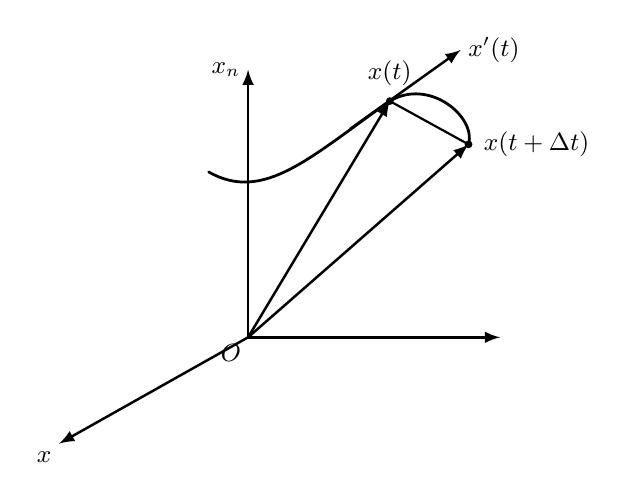
\begin{tikzpicture}[x=1.0cm, y=1.0cm, >=latex, line cap=round, line join=round]
    \draw[line width=0.9pt, ->] (0, 0) -- (-2.4, -1.35) node[below left=-1pt] {\small $x$};
    \draw[line width=0.9pt, ->] (0, 0) -- (3.2, 0);
    \draw[line width=0.9pt, ->] (0, 0) -- (0, 3.4) node[left=-1pt] {\small $x_n$};
    \node[below left=-1pt] at (0, 0) {\small $O$};

    \draw[line width=1.0pt] (-0.5, 2.1) .. controls (0.2, 1.7) and (0.8, 2.3) .. (1.8, 3.0)
                            .. controls (2.3, 3.3) and (2.9, 2.8) .. (2.8, 2.45);

    \coordinate (P) at (1.8, 3.0);
    \coordinate (Q) at (2.8, 2.45);

    \draw[line width=0.9pt, ->] (0, 0) -- (P);
    \draw[line width=0.9pt, ->] (0, 0) -- (Q);
    \draw[line width=0.8pt] (P) -- (Q);

    \draw[line width=0.9pt, ->] (1.3, 2.65) -- (2.7, 3.65) node[right=-1pt] {\small $\boldsymbol{x}'(t)$};

    \fill (P) circle (1.4pt) node[above=2pt] {\small $\boldsymbol{x}(t)$};
    \fill (Q) circle (1.4pt) node[right=2pt] {\small $\boldsymbol{x}(t + \Delta t)$};
  \end{tikzpicture}
  \caption{}\label{fig:9.1.1}
\end{figure}

我们称 $\boldsymbol{x}^{\prime}(t)$ 为曲线 $\boldsymbol{x}(t)$ 在 $t$ 点处的切向量. 当 $t$ 变动时, 得到一个沿曲线 $\boldsymbol{x}(t)$ 的切向量场. 如果 $\boldsymbol{x}(t)$ 为正则曲线, 则 $\dfrac{\boldsymbol{x}^{\prime}(t)}{\|\boldsymbol{x}^{\prime}(t)\|}$ 为沿曲线 $\boldsymbol{x}(t)$ 的单位切向量场. 应该强调的是 $\boldsymbol{x}^{\prime}(t)$ 或 $\dfrac{\boldsymbol{x}^{\prime}(t)}{\|\boldsymbol{x}^{\prime}(t)\|}$ 都是从 $\boldsymbol{x}(t)$ 点出发的向量.

\begin{definition}\label{def:9.1.2}
设 $\boldsymbol{x}(\boldsymbol{u})$ 为 $s$ 维 $C^{k}\,(k \geqslant 1)$ 正则曲面(也记为 $M$), 称 $\boldsymbol{x}'_{u_i}$ 为关于参数坐标 $u_{i}$ 的坐标切向量, 它是 $u_{i}$ 曲线(固定所有参数 $u_{j}\,(j \neq i)$, 只让 $u_{i}$ 变动时的曲线)的切向量. 由于 $\boldsymbol{x}(\boldsymbol{u})$ 为正则曲面, 故 $\operatorname{rank}(\boldsymbol{x}'_{u_1}, \boldsymbol{x}'_{u_2}, \cdots, \boldsymbol{x}'_{u_s}) = s$, 即 $\boldsymbol{x}'_{u_1}, \boldsymbol{x}'_{u_2}, \cdots, \boldsymbol{x}'_{u_s}$ 是线性无关的. 我们称由 $\{\boldsymbol{x}'_{u_1}(\boldsymbol{u}^0), \boldsymbol{x}'_{u_2}(\boldsymbol{u}^0), \cdots, \boldsymbol{x}'_{u_s}(\boldsymbol{u}^0)\}$ 张成的线性子空间
\[
  T_{\boldsymbol{x}(\boldsymbol{u}^{0})}M = \Big\{\sum_{i=1}^{s}\alpha_{i}\boldsymbol{x}_{u_{i}}^{\prime}(\boldsymbol{u}^{0}) \mathrel{\Big|} \alpha_{i} \in \mathbb{R}\Big\}
\]
为曲面 $M$(或 $\boldsymbol{x}(\boldsymbol{u})$)在点 $\boldsymbol{x}(\boldsymbol{u}^{0})$ 处的切空间. $T_{\boldsymbol{x}(\boldsymbol{u}^{0})}M$ 的每个向量称为曲面 $M$ 在点 $\boldsymbol{x}(\boldsymbol{u}^{0})$ 处的切向量. 显然, $T_{\boldsymbol{x}(\boldsymbol{u}^{0})}M$ 为 $s$ 维线性(向量)空间.
\end{definition}

\begin{theorem}\label{thm:9.1.1}
设 $\boldsymbol{x}(\boldsymbol{u})$ 在 $\boldsymbol{u}^{0} \in \Delta$ 处可微, 如果 $\{\boldsymbol{x}_{u_{1}}^{\prime}(\boldsymbol{u}^{0}), \boldsymbol{x}_{u_{2}}^{\prime}(\boldsymbol{u}^{0}), \cdots, \boldsymbol{x}_{u_{s}}^{\prime}(\boldsymbol{u}^{0})\}$ 线性无关, 即 $\operatorname{rank}\{\boldsymbol{x}_{u_{1}}^{\prime}(\boldsymbol{u}^{0}), \boldsymbol{x}_{u_{2}}^{\prime}(\boldsymbol{u}^{0}), \cdots, \boldsymbol{x}_{u_{s}}^{\prime}(\boldsymbol{u}^{0})\} = s$, $\boldsymbol{u}^{0} = \boldsymbol{u}(0)$ 为 $\boldsymbol{u}(t)$ 上一固定点, $\boldsymbol{u}(t)$ 在点 $0$ 处可导, 则
\[
  \frac{\mathrm{d}\boldsymbol{x}(\boldsymbol{u}(t))}{\mathrm{d}t}\bigg|_{t_0} \in T_{\boldsymbol{x}(\boldsymbol{u}^{0})}M,
\]
其中 $M = \boldsymbol{x}(\Delta)$(见\cref{def:9.1.1}).

反之, $\forall \boldsymbol{\alpha} \in \mathbb{R}^{s}$, $\sum_{i=1}^{s} \alpha_{i} \boldsymbol{x}_{u_{i}}^{\prime}(\boldsymbol{u}^{0}) \in T_{\boldsymbol{x}(\boldsymbol{u}^{0})}M$, 必 $\exists \boldsymbol{x}(\boldsymbol{u}(t)) \in M$, s.t. $\boldsymbol{u}(0) = \boldsymbol{u}^{0}$, 且
\[
  \frac{\mathrm{d}\boldsymbol{x}(\boldsymbol{u}(t))}{\mathrm{d}t}\bigg|_{t_0} = \sum_{i=1}^{s}\alpha_{i}\boldsymbol{x}_{u_{i}}^{\prime}(\boldsymbol{u}^{0}).
\]
这表明切空间 $T_{\boldsymbol{x}(\boldsymbol{u}^{0})}M$ 中的任一切向量都可用上述方式得到.
\end{theorem}

\begin{proof}
由于 $\boldsymbol{x}(\boldsymbol{u})$ 在 $\boldsymbol{u}^{0} = \boldsymbol{u}(0)$ 处可微, $\boldsymbol{u}(t)$ 在 $t = 0$ 处可导, 根据定理 8.2.2 与定理 8.2.6 知,
\[
  \frac{\mathrm{d}\boldsymbol{x}(\boldsymbol{u}(t))}{\mathrm{d}t}\bigg|_{t=0} = \sum_{i=1}^{s}\boldsymbol{x}_{u_{i}}^{\prime}(\boldsymbol{u}(0))u_{i}^{\prime}(0) = \sum_{i=1}^{s}u_{i}^{\prime}(0)\boldsymbol{x}_{u_{i}}^{\prime}(\boldsymbol{u}^{0}) \in T_{\boldsymbol{x}(\boldsymbol{u}^{0})}M.
\]
反之, $\forall \boldsymbol{\alpha} \in \mathbb{R}^s$, 令 $\boldsymbol{u}(t) = \boldsymbol{u}^0 + t\boldsymbol{\alpha}$, 则
\[
  \frac{\mathrm{d}\boldsymbol{x}(\boldsymbol{u}^{0} + t\boldsymbol{\alpha})}{\mathrm{d}t}\bigg|_{t=0} = \sum_{i=1}^{s}\alpha_{i}\boldsymbol{x}_{u_{i}}^{\prime}(\boldsymbol{u}^{0}) \in T_{\boldsymbol{x}(\boldsymbol{u}^{0})}M. \qedhere
\]
\end{proof}

曲面 $M$ 在点 $\boldsymbol{x}(\boldsymbol{u}^{0})$ 处的每个切向量 $\sum_{i=1}^{s}\alpha_{i}\boldsymbol{x}_{u_{i}}^{\prime}(\boldsymbol{u}^{0})$ 的起点都为 $\boldsymbol{x}(\boldsymbol{u}^{0})$, 其终点在 $\mathbb{R}^{n}$ 中可表示为(\cref{fig:9.1.2})
\[
  \boldsymbol{y} = \boldsymbol{x}(\boldsymbol{u}^{0}) + \sum_{i=1}^{s}\alpha_{i}\boldsymbol{x}_{u_{i}}^{\prime}(\boldsymbol{u}^{0}).
\]

\begin{figure}[htbp]
  \centering
  \begin{tikzpicture}[x=1.0cm, y=1.0cm, >=latex, line cap=round, line join=round]
    \draw[line width=0.9pt, ->] (0, 0) -- (-1.8, -1.2) node[below left=-1pt] {\small $x_1$};
    \draw[line width=0.9pt, ->] (0, 0) -- (4.0, 0) node[below=-1pt] {\small $x_2$};
    \draw[line width=0.9pt, ->] (0, 0) -- (0, 3.8) node[left=-1pt] {\small $x_3$};
    \node[below left=-1pt] at (0, 0) {\small $O$};

    \draw[line width=1.0pt] (0.8, 2.6) .. controls (1.5, 3.8) and (3.3, 3.6) .. (4.5, 2.8);
    \draw[line width=1.0pt] (0.8, 2.6) .. controls (1.2, 2.1) and (2.0, 2.4) .. (2.6, 2.0)
                            .. controls (3.2, 1.6) and (3.6, 0.9) .. (3.8, 1.0)
                            .. controls (4.0, 1.8) and (4.4, 2.1) .. (4.5, 2.8);
    \node at (4.0, 2.2) {\small $M$};

    \coordinate (X0) at (2.2, 2.6);

    \coordinate (PL1) at (1.8, 2.1);
    \coordinate (PL2) at (4.7, 2.4);
    \coordinate (PL3) at (4.9, 4.3);
    \coordinate (PL4) at (2.0, 4.0);
    \draw[line width=0.9pt] (PL1) -- (PL2) -- (PL3) -- (PL4) -- cycle;

    \draw[line width=0.7pt, dashed] (0, 0) -- ($(0,0)!0.65!(X0)$);
    \draw[line width=0.7pt] ($(0,0)!0.65!(X0)$) -- (X0);

    \draw[line width=1.0pt, ->] (X0) -- ++(1.4, 0.08) node[right=-1pt] {\small $\boldsymbol{x}'_{u_1}(\boldsymbol{u}^0)$};
    \draw[line width=1.0pt, ->] (X0) -- ++(0.15, 1.4) node[above=-1pt] {\small $\boldsymbol{x}'_{u_2}(\boldsymbol{u}^0)$};

    \coordinate (Y) at ($(X0) + (1.2, 1.1)$);
    \draw[line width=0.9pt, ->] (X0) -- (Y);
    \draw[line width=0.7pt, dashed] (0, 0) -- ($(0,0)!0.65!(Y)$);
    \draw[line width=0.7pt] ($(0,0)!0.65!(Y)$) -- (Y);

    \node[anchor=south west, inner sep=1pt] at (3.3, 3.4) {
      \small $\begin{aligned}
        &T_{\boldsymbol{x}(\boldsymbol{u}^0)}M \\
        &\boldsymbol{y} = \boldsymbol{x}(\boldsymbol{u}^0) + \sum_{i=1}^2 \alpha_i \boldsymbol{x}'_{u_i}(\boldsymbol{u}^0)
      \end{aligned}$
    };

    \fill (X0) circle (1.4pt) node[below=2pt] {\small $\boldsymbol{x}(\boldsymbol{u}^0)$};
  \end{tikzpicture}
  \caption{}\label{fig:9.1.2}
\end{figure}

\begin{example}\label{ex:9.1.1}
设 $\boldsymbol{x}\colon (a,b) \to \mathbb{R}^n$ 为 $C^k\,(k \geqslant 1)$ 正则曲线, 记为 $M$. $t_0 \in (a,b)$, 曲线 $\boldsymbol{x}(t)$ 在 $t_0$ 的切向量为 $\boldsymbol{x}'(t_0)$, 切空间 $T_{\boldsymbol{x}(t_0)} M = \{\alpha \boldsymbol{x}'(t_0) \mid \alpha \in \mathbb{R}\}$. 在 $\boldsymbol{x}(t_0)$ 处的切线为 $\boldsymbol{y} = \boldsymbol{x}(t_0) + \alpha \boldsymbol{x}'(t_0)$(向量形式), $\boldsymbol{x}(t_0)$ 为切线上的定点, $\boldsymbol{y}$ 为切线上的动点, $\alpha$ 为切线上的参数(\cref{fig:9.1.3}). 或坐标形式为
\[
  \frac{y_{1} - x_{1}(t_{0})}{x_{1}^{\prime}(t_{0})} = \frac{y_{2} - x_{2}(t_{0})}{x_{2}^{\prime}(t_{0})} = \cdots = \frac{y_{n} - x_{n}(t_{0})}{x_{n}^{\prime}(t_{0})} \, (=\alpha).
\]
\end{example}

\begin{figure}[htbp]
  \centering
  \begin{tikzpicture}[x=1.0cm, y=1.0cm, >=latex, line cap=round, line join=round]
    \draw[line width=0.9pt, ->] (0, 0) -- (-1.8, -1.2) node[below left=-1pt] {\small $x_1$};
    \draw[line width=0.9pt, ->] (0, 0) -- (3.8, 0) node[below=-1pt] {\small $x_2$};
    \draw[line width=0.9pt, ->] (0, 0) -- (0, 3.5) node[left=-1pt] {\small $y$};
    \node[below left=-1pt] at (0, 0) {\small $O$};

    \coordinate (X0) at (1.6, 2.3);

    \coordinate (N1) at (1.2, 3.5);
    \coordinate (N2) at (2.4, 2.7);
    \coordinate (N3) at (2.2, 0.4);
    \coordinate (N4) at (1.0, 1.2);
    \draw[line width=1.1pt] (N1) -- (N2) -- (N3) -- (N4) -- cycle;
    \node at (1.7, 1.4) {\small 法平面};

    \draw[line width=0.9pt] (0.5, 1.4) .. controls (1.1, 1.8) and (1.4, 2.2) .. (X0);
    \draw[line width=0.9pt] (X0) .. controls (1.9, 2.4) and (2.3, 2.7) .. (2.7, 2.6)
                            .. controls (3.1, 2.5) and (3.3, 2.1) .. (3.1, 1.6);
    \node[right=2pt] at (2.6, 2.1) {\small $\boldsymbol{x}(t)$};

    \draw[line width=0.8pt] (0.8, 1.7) -- ($(X0)!0.4!(0.8, 1.7)$);
    \draw[line width=0.8pt, dashed] ($(X0)!0.4!(0.8, 1.7)$) -- (X0);
    \draw[line width=0.8pt, dashed] (X0) -- ($(X0)!0.3!(3.0, 3.2)$);
    \draw[line width=0.9pt, ->] ($(X0)!0.3!(3.0, 3.2)$) -- (3.0, 3.2);
    \node[anchor=west] at (3.0, 3.2) {\small $\boldsymbol{y} = \boldsymbol{x}(t_0) + \alpha \boldsymbol{x}'(t_0)$};

    \draw[line width=0.8pt] (0.5, 2.6) -- (3.0, 1.2);
    \node[below right] at (2.7, 1.3) {\small 割线};

    \draw[line width=0.5pt, ->] (3.8, 3.7) node[right] {\small 切线} -- (3.05, 3.25);
    \draw[line width=0.5pt, ->] (2.2, 3.3) node[above] {\small 切方向} -- (X0);

    \fill (X0) circle (1.4pt) node[above left=-1pt] {\small $\boldsymbol{x}(t_0)$};
  \end{tikzpicture}
  \caption{}\label{fig:9.1.3}
\end{figure}

垂直切向量的超平面
\[
  x_{1}^{\prime}(t_{0})(y_{1} - x_{1}(t_{0})) + x_{2}^{\prime}(t_{0})(y_{2} - x_{2}(t_{0})) + \cdots + x_{n}^{\prime}(t_{0})(y_{n} - x_{n}(t_{0})) = 0
\]
称为曲线 $\boldsymbol{x}(t)$ 在 $\boldsymbol{x}(t_{0})$ 处的法平面. $\boldsymbol{x}(t_{0})$ 为法平面上的定点, 而 $\boldsymbol{y} = (y_{1}, y_{2}, \cdots, y_{n})$ 为法平面上的动点.

\begin{example}\label{ex:9.1.2}
设 $\Delta \subset \mathbb{R}^{2}$ 为开集, $\boldsymbol{x}\colon \Delta \to \mathbb{R}^{3}$, $(u, v) \mapsto \boldsymbol{x}(u, v) = (x(u, v), y(u, v), z(u, v))$ 为 $C^{k}\,(k \geqslant 1)$ 映射, $\operatorname{rank}(\boldsymbol{x}_{u}^{\prime}, \boldsymbol{x}_{v}^{\prime}) = 2$, $M = \boldsymbol{x}(\Delta)$ 为一个二维 $C^{k}$ 正则超曲面, 它的切空间为 $T_{\boldsymbol{x}(u,v)} M = \{\alpha_{1} \boldsymbol{x}_{u}^{\prime}(u, v) + \alpha_{2} \boldsymbol{x}_{v}^{\prime}(u, v) \mid \alpha_{1}, \alpha_{2} \in \mathbb{R}\}$.

在 $\boldsymbol{x}(u,v)$ 处的切超平面为(向量形式)
\[
  \boldsymbol{y} = \boldsymbol{x}(u,v) + \alpha_{1}\boldsymbol{x}_{u}^{\prime}(u,v) + \alpha_{2}\boldsymbol{x}_{v}^{\prime}(u,v).
\]
$\boldsymbol{x}(u,v)$ 为切超平面上的定点, $\boldsymbol{y}$ 为切超平面上的动点, $\alpha_{1}, \alpha_{2}$ 为切超平面上的参数.

与切超平面中从点 $\boldsymbol{x}(u,v)$ 出发的任何切向量 $\alpha_{1}\boldsymbol{x}'_{u}(u,v) + \alpha_{2}\boldsymbol{x}'_{v}(u,v)$ 都正交的向量称为 $\boldsymbol{x}(u,v)$ 点处的法向量. 显然, $\boldsymbol{n}$ 为法向量等价于 $\boldsymbol{n}$ 与 $\boldsymbol{x}'_{u}(u,v)$, $\boldsymbol{x}'_{v}(u,v)$ 都正交.

例如(\cref{fig:9.1.4}),
\begin{align*}
  \boldsymbol{n}(u,v) &= \boldsymbol{x}_{u}^{\prime}(u,v) \times \boldsymbol{x}_{v}^{\prime}(u,v) = \begin{vmatrix}
    \boldsymbol{i} & \boldsymbol{j} & \boldsymbol{k} \\
    \dfrac{\partial x}{\partial u} & \dfrac{\partial y}{\partial u} & \dfrac{\partial z}{\partial u} \\
    \dfrac{\partial x}{\partial v} & \dfrac{\partial y}{\partial v} & \dfrac{\partial z}{\partial v}
  \end{vmatrix} \\
  &= \frac{\partial(y,z)}{\partial(u,v)}\boldsymbol{i} + \frac{\partial(z,x)}{\partial(u,v)}\boldsymbol{j} + \frac{\partial(x,y)}{\partial(u,v)}\boldsymbol{k}
\end{align*}
或等于 $\left(\dfrac{\partial(y,z)}{\partial(u,v)}, \dfrac{\partial(z,x)}{\partial(u,v)}, \dfrac{\partial(x,y)}{\partial(u,v)}\right)$, 它既与 $\boldsymbol{x}_{u}^{\prime}(u,v)$ 正交, 又与 $\boldsymbol{x}_{v}^{\prime}(u,v)$ 正交. 因此, 上述的 $\boldsymbol{n}(u,v)$ 为超曲面 $M$ 在点 $\boldsymbol{x}(u,v)$ 处的法向量. 而切超平面的另一向量形式为
\[
  (\boldsymbol{y} - \boldsymbol{x}(u,v)) \cdot \boldsymbol{n}(u,v) = 0,
\]
其坐标形式为
\[
  \begin{vmatrix}
    y_{1} - x(u,v) & y_{2} - y(u,v) & y_{3} - z(u,v) \\
    \dfrac{\partial x}{\partial u} & \dfrac{\partial y}{\partial u} & \dfrac{\partial z}{\partial u} \\
    \dfrac{\partial x}{\partial v} & \dfrac{\partial y}{\partial v} & \dfrac{\partial z}{\partial v}
  \end{vmatrix} = 0.
\]
\end{example}

\begin{figure}[htbp]
  \centering
  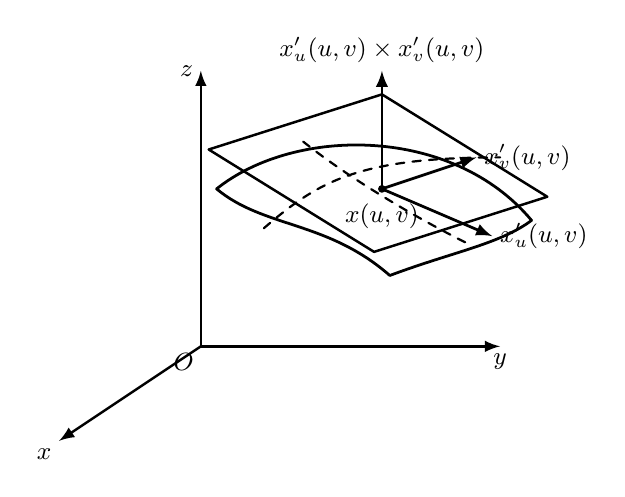
\begin{tikzpicture}[x=1.0cm, y=1.0cm, >=latex, line cap=round, line join=round]
    \draw[line width=0.9pt, ->] (0, 0) -- (-1.8, -1.2) node[below left=-1pt] {\small $x$};
    \draw[line width=0.9pt, ->] (0, 0) -- (3.8, 0) node[below=-1pt] {\small $y$};
    \draw[line width=0.9pt, ->] (0, 0) -- (0, 3.5) node[left=-1pt] {\small $z$};
    \node[below left=-1pt] at (0, 0) {\small $O$};

    \draw[line width=1.0pt] (0.2, 2.0) .. controls (1.2, 2.8) and (3.2, 2.8) .. (4.2, 1.6);
    \draw[line width=1.0pt] (0.2, 2.0) .. controls (0.8, 1.5) and (1.6, 1.6) .. (2.4, 0.9)
                            .. controls (3.2, 1.2) and (3.8, 1.3) .. (4.2, 1.6);

    \coordinate (XUV) at (2.3, 2.0);
    \draw[line width=0.8pt, dashed] (0.8, 1.5) .. controls (1.5, 2.1) and (2.0, 2.4) .. (3.8, 2.4);
    \draw[line width=0.8pt, dashed] (1.3, 2.6) .. controls (1.8, 2.2) and (2.6, 1.7) .. (3.4, 1.3);

    \coordinate (TP1) at (0.1, 2.5);
    \coordinate (TP2) at (2.2, 1.2);
    \coordinate (TP3) at (4.4, 1.9);
    \coordinate (TP4) at (2.3, 3.2);
    \draw[line width=0.9pt] (TP1) -- (TP2) -- (TP3) -- (TP4) -- cycle;

    \draw[line width=1.0pt, ->] (XUV) -- ++(1.4, -0.6) node[right=-1pt] {\small $\boldsymbol{x}'_u(u,v)$};
    \draw[line width=1.0pt, ->] (XUV) -- ++(1.2, 0.4) node[right=-1pt] {\small $\boldsymbol{x}'_v(u,v)$};
    \draw[line width=1.0pt, ->] (XUV) -- ++(0, 1.5) node[above=-1pt] {\small $\boldsymbol{x}'_u(u,v) \times \boldsymbol{x}'_v(u,v)$};

    \fill (XUV) circle (1.4pt) node[below=2pt] {\small $\boldsymbol{x}(u,v)$};
  \end{tikzpicture}
  \caption{}\label{fig:9.1.4}
\end{figure}

$\boldsymbol{n}(u,v)$ 通常不是单位向量. 现在, 我们来计算它的模. 由于
\begin{align*}
  \|\boldsymbol{x}_{u}^{\prime} \times \boldsymbol{x}_{v}^{\prime}\|^{2}
  &= (\|\boldsymbol{x}_{u}^{\prime}\| \|\boldsymbol{x}_{v}^{\prime}\| \sin\theta)^{2} \\
  &= \|\boldsymbol{x}_{u}^{\prime}\|^{2} \|\boldsymbol{x}_{v}^{\prime}\|^{2} (1 - \cos^{2}\theta) \\
  &= \|\boldsymbol{x}_{u}^{\prime}\|^{2} \|\boldsymbol{x}_{v}^{\prime}\|^{2} - (\boldsymbol{x}_{u}^{\prime} \cdot \boldsymbol{x}_{v}^{\prime})^{2} = EG - F^{2} = \det\begin{pmatrix} E & F \\ F & G \end{pmatrix},
\end{align*}
其中
\[
  \left\{\begin{aligned}
    E &= \boldsymbol{x}_{u}^{\prime} \cdot \boldsymbol{x}_{u}^{\prime} = \left(\frac{\partial x}{\partial u}\right)^{2} + \left(\frac{\partial y}{\partial u}\right)^{2} + \left(\frac{\partial z}{\partial u}\right)^{2}, \\
    F &= \boldsymbol{x}_{u}^{\prime} \cdot \boldsymbol{x}_{v}^{\prime} = \frac{\partial x}{\partial u}\frac{\partial x}{\partial v} + \frac{\partial y}{\partial u}\frac{\partial y}{\partial v} + \frac{\partial z}{\partial u}\frac{\partial z}{\partial v}, \\
    G &= \boldsymbol{x}_{v}^{\prime} \cdot \boldsymbol{x}_{v}^{\prime} = \left(\frac{\partial x}{\partial v}\right)^{2} + \left(\frac{\partial y}{\partial v}\right)^{2} + \left(\frac{\partial z}{\partial v}\right)^{2}.
  \end{aligned}\right.
\]
因此, $\boldsymbol{x}(u,v)$ 处的单位法向量为
\[
  \boldsymbol{n}_{0} = \pm\frac{\boldsymbol{x}_{u}^{\prime} \times \boldsymbol{x}_{v}^{\prime}}{\|\boldsymbol{x}_{u}^{\prime} \times \boldsymbol{x}_{v}^{\prime}\|} = \pm\frac{1}{\sqrt{EG - F^{2}}}\left(\frac{\partial(y,z)}{\partial(u,v)}, \frac{\partial(z,x)}{\partial(u,v)}, \frac{\partial(x,y)}{\partial(u,v)}\right).
\]
$E, F, G$ 称为曲面 $M$ 的第一基本量.

设参数 $(u,v)$ 与参数 $(\bar{u},\bar{v})$ 之间存在着一一对应的、一阶连续可导的对应关系
\[
  \left\{\begin{aligned}
    u &= u(\bar{u}, \bar{v}), \\
    v &= v(\bar{u}, \bar{v}),
  \end{aligned}\right. \quad (\bar{u}, \bar{v}) \in \bar{\Delta}, \; (u, v) \in \Delta.
\]
这时曲面 $M$ 有了新的参数表示:
\[
  \boldsymbol{x} = \boldsymbol{x}(u(\bar{u}, \bar{v}), v(\bar{u}, \bar{v})).
\]
直接的计算可知
\begin{align*}
  \bar{\boldsymbol{n}}(\bar{u}, \bar{v}) &= \boldsymbol{x}^{\prime}_{\bar{u}} \times \boldsymbol{x}^{\prime}_{\bar{v}} = \Big(\boldsymbol{x}^{\prime}_{u}\frac{\partial u}{\partial\bar{u}} + \boldsymbol{x}^{\prime}_{v}\frac{\partial v}{\partial\bar{u}}\Big) \times \Big(\boldsymbol{x}^{\prime}_{u}\frac{\partial u}{\partial\bar{v}} + \boldsymbol{x}^{\prime}_{v}\frac{\partial v}{\partial\bar{v}}\Big) \\
  &= \Big(\frac{\partial u}{\partial\bar{u}}\frac{\partial v}{\partial\bar{v}} - \frac{\partial u}{\partial\bar{v}}\frac{\partial v}{\partial\bar{u}}\Big)\boldsymbol{x}^{\prime}_{u} \times \boldsymbol{x}^{\prime}_{v} \\
  &= \frac{\partial(u,v)}{\partial(\bar{u},\bar{v})}\boldsymbol{x}^{\prime}_{u} \times \boldsymbol{x}^{\prime}_{v} = \frac{\partial(u,v)}{\partial(\bar{u},\bar{v})}\boldsymbol{n}(u,v).
\end{align*}
注意, 由于
\[
  1 = \frac{\partial(u,v)}{\partial(u,v)} = \frac{\partial(u,v)}{\partial(\bar{u},\bar{v})}\frac{\partial(\bar{u},\bar{v})}{\partial(u,v)},
\]
故
\[
  \frac{\partial(u,v)}{\partial(\bar{u},\bar{v})} \neq 0, \quad \frac{\partial(\bar{u},\bar{v})}{\partial(u,v)} \neq 0.
\]
如果 $\dfrac{\partial(u,v)}{\partial(\bar{u},\bar{v})} > 0\,(< 0)$, 则 $\bar{\boldsymbol{n}}(\bar{u},\bar{v})$ 与 $\boldsymbol{n}(u,v)$ 同(反)向, 我们称 $(\bar{u},\bar{v})$ 与 $(u,v)$ 为同(反)向的参数.

更一般地, 我们有下面结果.

\begin{example}\label{ex:9.1.3}
设 $\Delta \subset \mathbb{R}^{n-1}$ 为开集,
\[
  \boldsymbol{x}\colon \Delta \to \mathbb{R}^{n}, \quad \boldsymbol{u} = (u_{1}, u_{2}, \cdots, u_{n-1}) \mapsto \boldsymbol{x}(\boldsymbol{u}) = (x_{1}(\boldsymbol{u}), x_{2}(\boldsymbol{u}), \cdots, x_{n}(\boldsymbol{u}))
\]
为 $C^{k}\,(k \geqslant 1)$ 映射, $\operatorname{rank}(\boldsymbol{x}_{u_{1}}^{\prime}, \boldsymbol{x}_{u_{2}}^{\prime}, \cdots, \boldsymbol{x}_{u_{n-1}}^{\prime}) = n - 1$, $M = \boldsymbol{x}(\Delta)$ 为一个 $n - 1$ 维 $C^{k}$ 正则超曲面, 它的切空间为
\[
  T_{\boldsymbol{x}(\boldsymbol{u})}M = \Big\{\sum_{i=1}^{n-1}\alpha_{i}\boldsymbol{x}_{u_{i}}^{\prime}(\boldsymbol{u}) \mathrel{\Big|} \alpha_{i} \in \mathbb{R}, \, i = 1, 2, \cdots, n - 1\Big\}.
\]
在 $\boldsymbol{x}(\boldsymbol{u})$ 处的切超平面为(向量形式)
\[
  \boldsymbol{y} = \boldsymbol{x}(\boldsymbol{u}) + \sum_{i=1}^{n-1}\alpha_{i}\boldsymbol{x}_{u_{i}}^{\prime}(\boldsymbol{u}).
\]
$\boldsymbol{x}(\boldsymbol{u})$ 为切超平面上的定点, $\boldsymbol{y}$ 为切超平面上的动点, $\alpha_{1}, \alpha_{2}, \cdots, \alpha_{n-1}$ 为切超平面上的参数.

与切超平面中从点 $\boldsymbol{x}(\boldsymbol{u})$ 出发的任何切向量 $\sum_{i=1}^{n-1}\alpha_i \boldsymbol{x}'_{u_i}(\boldsymbol{u})$ 都正交的向量称为 $\boldsymbol{x}(\boldsymbol{u})$ 点处的法向量. 显然,
\[
  \boldsymbol{n} \text{ 为法向量} \iff \boldsymbol{n} \text{ 与每个 } \boldsymbol{x}'_{u_i}\,(i = 1, 2, \cdots, n - 1) \text{ 都正交}.
\]
例如, 设 $\{\boldsymbol{e}_{1}, \boldsymbol{e}_{2}, \cdots, \boldsymbol{e}_{n}\}$ 为 $\mathbb{R}^{n}$ 中的规范正交基(当 $n = 3$ 时, $\boldsymbol{e}_{1} = \boldsymbol{i}$, $\boldsymbol{e}_{2} = \boldsymbol{j}$, $\boldsymbol{e}_{3} = \boldsymbol{k}$), 则
\[
  \boldsymbol{n}(\boldsymbol{u}) = \begin{vmatrix}
    \boldsymbol{e}_{1} & \cdots & \boldsymbol{e}_{n} \\
    \dfrac{\partial x_{1}}{\partial u_{1}} & \cdots & \dfrac{\partial x_{n}}{\partial u_{1}} \\
    \vdots & & \vdots \\
    \dfrac{\partial x_{1}}{\partial u_{n-1}} & \cdots & \dfrac{\partial x_{n}}{\partial u_{n-1}}
  \end{vmatrix} = \sum_{i=1}^{n}(-1)^{1+i}\frac{\partial(x_{1}, x_{2}, \cdots, \hat{x}_{i}, \cdots, x_{n})}{\partial(u_{1}, u_{2}, \cdots, u_{n-1})}\boldsymbol{e}_{i}
\]
与每个 $\dfrac{\partial\boldsymbol{x}}{\partial u_{i}}$ 正交 $(i = 1, 2, \cdots, n - 1)$, 其中 $\hat{x}_{i}$ 表示删去 $x_{i}$. 换言之,
\[
  \boldsymbol{n}(\boldsymbol{u}) \cdot \frac{\partial\boldsymbol{x}}{\partial u_{i}} = \begin{vmatrix}
    \dfrac{\partial x_{1}}{\partial u_{i}} & \cdots & \dfrac{\partial x_{n}}{\partial u_{i}} \\
    \dfrac{\partial x_{1}}{\partial u_{1}} & \cdots & \dfrac{\partial x_{n}}{\partial u_{1}} \\
    \vdots & & \vdots \\
    \dfrac{\partial x_{1}}{\partial u_{n-1}} & \cdots & \dfrac{\partial x_{n}}{\partial u_{n-1}}
  \end{vmatrix} = 0.
\]
因此, 上述的 $\boldsymbol{n}(\boldsymbol{u})$ 为超曲面 $M$ 在点 $\boldsymbol{x}(\boldsymbol{u})$ 处的法向量, 而切超平面的另一向量形式为
\[
  (\boldsymbol{y} - \boldsymbol{x}(\boldsymbol{u})) \cdot \boldsymbol{n}(\boldsymbol{u}) = 0,
\]
其坐标形式为
\[
  \begin{vmatrix}
    y_{1} - x_{1}(\boldsymbol{u}) & \cdots & y_{n} - x_{n}(\boldsymbol{u}) \\
    \dfrac{\partial x_{1}}{\partial u_{1}} & \cdots & \dfrac{\partial x_{n}}{\partial u_{1}} \\
    \vdots & & \vdots \\
    \dfrac{\partial x_{1}}{\partial u_{n-1}} & \cdots & \dfrac{\partial x_{n}}{\partial u_{n-1}}
  \end{vmatrix} = 0.
\]
$\boldsymbol{n}(\boldsymbol{u})$ 通常不是单位向量. 当 $n \neq 3$ 时, 不能用 $\|\boldsymbol{x}'_{u} \times \boldsymbol{x}'_{v}\|$ 的方法来求 $\boldsymbol{n}(\boldsymbol{u})$ 的模. 但由其结果 $\|\boldsymbol{x}_{u}^{\prime} \times \boldsymbol{x}_{v}^{\prime}\|^{2} = \det\begin{pmatrix} E & F \\ F & G \end{pmatrix}$ 的启发, 我们有如下推导:

设 $g_{ij} = \boldsymbol{x}'_{u_i} \cdot \boldsymbol{x}'_{u_j} = \sum_{l=1}^{n} \dfrac{\partial x_l}{\partial u_i}\dfrac{\partial x_l}{\partial u_j}$, $i, j = 1, 2, \cdots, n - 1$. 则
\begin{align*}
  \|\boldsymbol{n}(\boldsymbol{u})\| &= \boldsymbol{n}(\boldsymbol{u}) \cdot \boldsymbol{n}_{0}(\boldsymbol{u}) = \begin{vmatrix}
    \boldsymbol{e}_{1} & \cdots & \boldsymbol{e}_{n} \\
    \dfrac{\partial x_{1}}{\partial u_{1}} & \cdots & \dfrac{\partial x_{n}}{\partial u_{1}} \\
    \vdots & & \vdots \\
    \dfrac{\partial x_{1}}{\partial u_{n-1}} & \cdots & \dfrac{\partial x_{n}}{\partial u_{n-1}}
  \end{vmatrix} \cdot \sum_{i=1}^{n}h_{i}\boldsymbol{e}_{i} \\
  &= \begin{vmatrix}
    h_{1} & \cdots & h_{n} \\
    \dfrac{\partial x_{1}}{\partial u_{1}} & \cdots & \dfrac{\partial x_{n}}{\partial u_{1}} \\
    \vdots & & \vdots \\
    \dfrac{\partial x_{1}}{\partial u_{n-1}} & \cdots & \dfrac{\partial x_{n}}{\partial u_{n-1}}
  \end{vmatrix} \\
  &= \sqrt{\det\begin{pmatrix}
    h_{1} & \cdots & h_{n} \\
    \dfrac{\partial x_{1}}{\partial u_{1}} & \cdots & \dfrac{\partial x_{n}}{\partial u_{1}} \\
    \vdots & & \vdots \\
    \dfrac{\partial x_{1}}{\partial u_{n-1}} & \cdots & \dfrac{\partial x_{n}}{\partial u_{n-1}}
  \end{pmatrix}\begin{pmatrix}
    h_{1} & \dfrac{\partial x_{1}}{\partial u_{1}} & \cdots & \dfrac{\partial x_{1}}{\partial u_{n-1}} \\
    \vdots & \vdots & & \vdots \\
    h_{n} & \dfrac{\partial x_{n}}{\partial u_{1}} & \cdots & \dfrac{\partial x_{n}}{\partial u_{n-1}}
  \end{pmatrix}} \\
  &= \sqrt{\det\begin{pmatrix}
    1 & 0 & \cdots & 0 \\
    0 & g_{11} & \cdots & g_{1,n-1} \\
    \vdots & \vdots & & \vdots \\
    0 & g_{n-1,1} & \cdots & g_{n-1,n-1}
  \end{pmatrix}} \\
  &= \sqrt{\det\begin{pmatrix}
    g_{11} & \cdots & g_{1,n-1} \\
    \vdots & & \vdots \\
    g_{n-1,1} & \cdots & g_{n-1,n-1}
  \end{pmatrix}} = \sqrt{\det(g_{ij})},
\end{align*}
其中 $\sum_{i=1}^{n}h_{i}\boldsymbol{e}_{i} = \boldsymbol{n}_{0}(\boldsymbol{u})$ 为与 $\boldsymbol{n}(\boldsymbol{u})$ 同方向的单位法向量. 因此, $\boldsymbol{x}(\boldsymbol{u})$ 处的单位法向量为
\[
  \boldsymbol{n}_{0}(\boldsymbol{u}) = \pm\frac{\boldsymbol{n}(\boldsymbol{u})}{\|\boldsymbol{n}(\boldsymbol{u})\|} = \pm\frac{1}{\sqrt{\det(g_{ij})}}\sum_{i=1}^{n}(-1)^{1+i}\frac{\partial(x_{1}, x_{2}, \cdots, \hat{x}_{i}, \cdots, x_{n})}{\partial(u_{1}, u_{2}, \cdots, u_{n-1})}\boldsymbol{e}_{i}.
\]
$g_{ij}\,(i, j = 1, 2, \cdots, n - 1)$ 称为超曲面 $M$ 的第一基本量. 当 $n = 3$ 时, $g_{11} = E$, $g_{12} = g_{21} = F$, $g_{22} = G$.

设参数 $(u_{1}, u_{2}, \cdots, u_{n-1})$ 与参数 $(\bar{u}_{1}, \bar{u}_{2}, \cdots, \bar{u}_{n-1})$ 之间存在着一一对应的、一阶连续可导的对应关系
\[
  \left\{\begin{aligned}
    u_{1} &= u_{1}(\bar{u}_{1}, \bar{u}_{2}, \cdots, \bar{u}_{n-1}), \\
    &\;\;\vdots \\
    u_{n-1} &= u_{n-1}(\bar{u}_{1}, \bar{u}_{2}, \cdots, \bar{u}_{n-1}),
  \end{aligned}\right. \quad \bar{\boldsymbol{u}} = (\bar{u}_{1}, \bar{u}_{2}, \cdots, \bar{u}_{n-1}) \in \bar{\Delta}, \; \boldsymbol{u} = (u_{1}, u_{2}, \cdots, u_{n-1}) \in \Delta.
\]
这时曲面 $M$ 有了新的参数表示:
\[
  \boldsymbol{x} = \boldsymbol{x}(\boldsymbol{u}(\bar{\boldsymbol{u}})) = \boldsymbol{x}(u_{1}(\bar{u}_{1}, \cdots, \bar{u}_{n-1}), u_{2}(\bar{u}_{1}, \cdots, \bar{u}_{n-1}), \cdots, u_{n-1}(\bar{u}_{1}, \cdots, \bar{u}_{n-1})).
\]
直接计算可知
\begin{align*}
  \bar{\boldsymbol{n}}(\bar{\boldsymbol{u}}) &= \begin{vmatrix}
    \boldsymbol{e}_{1} & \cdots & \boldsymbol{e}_{n} \\
    \dfrac{\partial x_{1}}{\partial\bar{u}_{1}} & \cdots & \dfrac{\partial x_{n}}{\partial\bar{u}_{1}} \\
    \vdots & & \vdots \\
    \dfrac{\partial x_{1}}{\partial\bar{u}_{n-1}} & \cdots & \dfrac{\partial x_{n}}{\partial\bar{u}_{n-1}}
  \end{vmatrix} = \sum_{i=1}^{n}(-1)^{1+i}\frac{\partial(x_{1}, x_{2}, \cdots, \hat{x}_{i}, \cdots, x_{n})}{\partial(\bar{u}_{1}, \bar{u}_{2}, \cdots, \bar{u}_{n-1})}\boldsymbol{e}_{i} \\
  &= \sum_{i=1}^{n}(-1)^{1+i}\frac{\partial(x_{1}, x_{2}, \cdots, \hat{x}_{i}, \cdots, x_{n})}{\partial(u_{1}, u_{2}, \cdots, u_{n-1})}\frac{\partial(u_{1}, u_{2}, \cdots, u_{n-1})}{\partial(\bar{u}_{1}, \bar{u}_{2}, \cdots, \bar{u}_{n-1})}\boldsymbol{e}_{i} \\
  &= \frac{\partial(u_{1}, u_{2}, \cdots, u_{n-1})}{\partial(\bar{u}_{1}, \bar{u}_{2}, \cdots, \bar{u}_{n-1})}\boldsymbol{n}(\boldsymbol{u}).
\end{align*}
\end{example}

注意, 由于
\[
  1 = \frac{\partial(u_{1}, u_{2}, \cdots, u_{n-1})}{\partial(u_{1}, u_{2}, \cdots, u_{n-1})} = \frac{\partial(u_{1}, u_{2}, \cdots, u_{n-1})}{\partial(\bar{u}_{1}, \bar{u}_{2}, \cdots, \bar{u}_{n-1})}\frac{\partial(\bar{u}_{1}, \bar{u}_{2}, \cdots, \bar{u}_{n-1})}{\partial(u_{1}, u_{2}, \cdots, u_{n-1})},
\]
故
\[
  \frac{\partial(u_{1}, u_{2}, \cdots, u_{n-1})}{\partial(\bar{u}_{1}, \bar{u}_{2}, \cdots, \bar{u}_{n-1})} \neq 0, \quad \frac{\partial(\bar{u}_{1}, \bar{u}_{2}, \cdots, \bar{u}_{n-1})}{\partial(u_{1}, u_{2}, \cdots, u_{n-1})} \neq 0.
\]
如果 $\dfrac{\partial(u_{1}, u_{2}, \cdots, u_{n-1})}{\partial(\bar{u}_{1}, \bar{u}_{2}, \cdots, \bar{u}_{n-1})} > 0\,(< 0)$, 则 $\bar{\boldsymbol{n}}(\bar{\boldsymbol{u}})$ 与 $\boldsymbol{n}(\boldsymbol{u})$ 同(反)向, 我们称 $(\bar{u}_{1}, \bar{u}_{2}, \cdots, \bar{u}_{n-1})$ 与 $(u_{1}, u_{2}, \cdots, u_{n-1})$ 为同(反)向的参数.

上面已详细讨论了 $C^{k}\,(k \geqslant 1)$ 正则超曲面的切空间, 法向量. 自然会问: $s$ 维 $C^{k}\,(k \geqslant 1)$ 的正则曲面的法空间应如何表示? 我们期望能用切空间 $T_{\boldsymbol{x}(\boldsymbol{u})}M$ 的基 $\{\boldsymbol{x}_{u_1}^{\prime}(\boldsymbol{u}),\allowbreak \boldsymbol{x}_{u_2}^{\prime}(\boldsymbol{u}),\allowbreak \cdots,\allowbreak \boldsymbol{x}_{u_s}^{\prime}(\boldsymbol{u})\}$ 来表达法空间
\[
  T_{\boldsymbol{x}(\boldsymbol{u})}^{\perp}M = \left\{\boldsymbol{n} \mathrel{\Big|} \boldsymbol{n} \perp T_{\boldsymbol{x}(\boldsymbol{u})}M, \text{ 即 } \boldsymbol{n} \cdot \boldsymbol{x}^{\prime}_{u_{i}}(\boldsymbol{u}) = 0, \, i = 1, 2, \cdots, s\right\},
\]
或者来表达法空间的一个基.

\begin{example}\label{ex:9.1.4}
设 $\boldsymbol{x}(\boldsymbol{u})$ 为 $s$ 维 $C^{k}\,(k \geqslant 1)$ 正则曲面, 则
\[
  (\boldsymbol{P} \quad \boldsymbol{Q}) = \begin{pmatrix}
    \dfrac{\partial\boldsymbol{x}(\boldsymbol{u})}{\partial u_{1}} \\
    \vdots \\
    \dfrac{\partial\boldsymbol{x}(\boldsymbol{u})}{\partial u_{s}}
  \end{pmatrix} = \begin{pmatrix}
    \dfrac{\partial x_{1}}{\partial u_{1}} & \cdots & \dfrac{\partial x_{n}}{\partial u_{1}} \\
    \vdots & & \vdots \\
    \dfrac{\partial x_{1}}{\partial u_{s}} & \cdots & \dfrac{\partial x_{n}}{\partial u_{s}}
  \end{pmatrix}.
\]
由于 $\operatorname{rank}(\boldsymbol{P} \quad \boldsymbol{Q}) = s$, 为叙述简单起见, 不妨设
\[
  \boldsymbol{P} = \begin{pmatrix}
    \dfrac{\partial x_{1}}{\partial u_{1}} & \cdots & \dfrac{\partial x_{s}}{\partial u_{1}} \\
    \vdots & & \vdots \\
    \dfrac{\partial x_{1}}{\partial u_{s}} & \cdots & \dfrac{\partial x_{s}}{\partial u_{s}}
  \end{pmatrix}
\]
为 $s \times s$ 非异矩阵. 因为
\begin{align*}
  (\boldsymbol{P} \quad \boldsymbol{Q})\left(-(\boldsymbol{P}^{-1}\boldsymbol{Q})^{\mathrm{T}} \quad \boldsymbol{I}_{n-s}\right)^{\mathrm{T}}
  &= (\boldsymbol{P} \quad \boldsymbol{Q})\begin{pmatrix} -\boldsymbol{P}^{-1}\boldsymbol{Q} \\ \boldsymbol{I}_{n-s} \end{pmatrix} \\
  &= -\boldsymbol{P}(\boldsymbol{P}^{-1}\boldsymbol{Q}) + \boldsymbol{Q}\boldsymbol{I}_{n-s} = -\boldsymbol{Q} + \boldsymbol{Q} = \boldsymbol{0},
\end{align*}
所以, $(\boldsymbol{P} \quad \boldsymbol{Q})$ 的行向量都正交于 $\left(-(\boldsymbol{P}^{-1}\boldsymbol{Q})^{\mathrm{T}} \quad \boldsymbol{I}_{n-s}\right)$ 的行向量. 此外, 显然有
\[
  \operatorname{rank}\left(-(\boldsymbol{P}^{-1}\boldsymbol{Q})^{\mathrm{T}} \quad \boldsymbol{I}_{n-s}\right) = n - s.
\]
因此, $\left(-(\boldsymbol{P}^{-1}\boldsymbol{Q})^{\mathrm{T}} \quad \boldsymbol{I}_{n-s}\right)$ 的 $n - s$ 个行向量为法空间 $T_{\boldsymbol{x}(\boldsymbol{u})}^{\perp}M$ 的一个基, 它由 $(\boldsymbol{P} \quad \boldsymbol{Q})$ 的元素所表达, 即由 $\dfrac{\partial x_{i}}{\partial u_{j}}\,(i = 1, 2, \cdots, n; \, j = 1, 2, \cdots, s)$ 所完全表达.
\end{example}

上述简洁的论述是难以想到的, 这是在查阅 Grassmann 流形 $G_{n-s,s}$ 与 $G_{s,n-s}$ 之间是微分同胚时, 见到的推导.

\begin{example}\label{ex:9.1.5}
设 $U \subset \mathbb{R}^n$ 为开集, $f\colon U \to \mathbb{R}^1$ 为 $C^k\,(1 \leqslant k \leqslant +\infty)$ 映射, 且在 $U$ 上,
\[
  \operatorname{rank} f = \operatorname{rank} \boldsymbol{J}f = \operatorname{rank}\left(\frac{\partial f}{\partial x_{1}}, \frac{\partial f}{\partial x_{2}}, \cdots, \frac{\partial f}{\partial x_{n}}\right) \equiv 1 \text{ (常值)},
\]
由例 8.4.5 知
\[
  M = f^{-1}(q) = \{\boldsymbol{x} \in U \mid f(\boldsymbol{x}) = q\} = \{\boldsymbol{x} \in U \mid f(\boldsymbol{x}) - q = 0\}
\]
{\emergencystretch=3em 或为空集, 或为 $n - 1$ 维 $C^{k}$ 流形或 $C^{k}$ 超曲面. 证明: 当 $M \neq \varnothing$ 时, $\operatorname{grad}f = \left(\dfrac{\partial f}{\partial x_{1}},\allowbreak \dfrac{\partial f}{\partial x_{2}},\allowbreak \cdots,\allowbreak \dfrac{\partial f}{\partial x_{n}}\right)$ 为 $M$ 的法向量场. 从而, 过定点 $\boldsymbol{x}^{0} \in M$ 的切超平面为\par}
\[
  (\boldsymbol{y} - \boldsymbol{x}^{0}) \cdot \operatorname{grad}f(\boldsymbol{x}^{0}) = 0,
\]
即
\[
  \sum_{i=1}^{n}\frac{\partial f}{\partial x_{i}}(\boldsymbol{x}^{0})(y_{i} - x_{i}^{0}) = 0.
\]
\end{example}

\begin{proof}[证法 1]
设 $M \neq \varnothing$, $\boldsymbol{x}(t)$ 为 $M$ 上过定点 $\boldsymbol{x}^{0} = \boldsymbol{x}(0)$ 的任一 $C^{1}$ 曲线, 则
\[
  f(\boldsymbol{x}(t)) \equiv q,
\]
两边对 $t$ 求导得到
\[
  \operatorname{grad}f \cdot \frac{\mathrm{d}\boldsymbol{x}}{\mathrm{d}t} = \sum_{i=1}^{n}\frac{\partial f}{\partial x_{i}}(\boldsymbol{x}(t))\frac{\mathrm{d}x_{i}}{\mathrm{d}t} \equiv 0,
\]
它表明 $f$ 的梯度向量 $\operatorname{grad}f \equiv \left(\dfrac{\partial f}{\partial x_{1}}, \dfrac{\partial f}{\partial x_{2}}, \cdots, \dfrac{\partial f}{\partial x_{n}}\right)\bigg|_{\boldsymbol{x}^{0}}$ 与曲面 $M$ 上点 $\boldsymbol{x}^{0}$ 处的切向量 $\boldsymbol{x}^{\prime}(0)$ 正交. 由于 $\boldsymbol{x}(t)$ 的任意性, $\operatorname{grad}f = \left(\dfrac{\partial f}{\partial x_{1}}, \dfrac{\partial f}{\partial x_{2}}, \cdots, \dfrac{\partial f}{\partial x_{n}}\right)\bigg|_{\boldsymbol{x}^{0}}$ 为 $T_{\boldsymbol{x}^{0}}M$ 的法向量.
\end{proof}

\begin{proof}[证法 2]
设 $M \neq \varnothing$, 不妨令 $\dfrac{\partial f}{\partial x_{n}} \neq 0$, 根据隐函数定理, 在局部, $x_{n} = x_{n}(x_{1}, x_{2}, \cdots, x_{n-1})$, 且
\[
  \frac{\partial x_{n}}{\partial x_{i}} = -\frac{\dfrac{\partial f}{\partial x_{i}}}{\dfrac{\partial f}{\partial x_{n}}}.
\]
由于局部参数表示为 $\boldsymbol{x} = \boldsymbol{x}(x_{1}, x_{2}, \cdots, x_{n-1}) = (x_{1}, x_{2}, \cdots, x_{n-1}, x_{n}(x_{1}, \cdots, x_{n-1}))$, 故
\[
  \left\{\begin{aligned}
    \boldsymbol{x}_{u_{1}}^{\prime} &= \left(1, 0, \cdots, 0, -\frac{\dfrac{\partial f}{\partial x_{1}}}{\dfrac{\partial f}{\partial x_{n}}}\right), \\
    &\;\;\vdots \\
    \boldsymbol{x}_{u_{n-1}}^{\prime} &= \left(0, 0, \cdots, 1, -\frac{\dfrac{\partial f}{\partial x_{n-1}}}{\dfrac{\partial f}{\partial x_{n}}}\right).
  \end{aligned}\right.
\]
显然,
\[
  \operatorname{grad}f \cdot \boldsymbol{x}_{u_{i}}^{\prime} = \left(\frac{\partial f}{\partial x_{1}}, \frac{\partial f}{\partial x_{2}}, \cdots, \frac{\partial f}{\partial x_{n}}\right) \cdot \left(0, \cdots, 0, \underset{\text{第 } i \text{ 个}}{1}, 0, \cdots, -\frac{\dfrac{\partial f}{\partial x_{i}}}{\dfrac{\partial f}{\partial x_{n}}}\right) = 0.
\]
因此, $\operatorname{grad}f = \left(\dfrac{\partial f}{\partial x_{1}}, \dfrac{\partial f}{\partial x_{2}}, \cdots, \dfrac{\partial f}{\partial x_{n}}\right)$ 为 $T_{\boldsymbol{x}(x_{1}, x_{2}, \cdots, x_{n-1})}M$ 的法向量. \qedhere
\end{proof}

\begin{definition}\label{def:9.1.3}
设 $\Delta_{i} \subset \mathbb{R}^{s_{i}}$ 为开集, $\varphi_{i}^{-1}\colon \Delta_{i} \to \varphi_{i}^{-1}(\Delta_{i}) \subset \mathbb{R}^{n_{i}}$ 为同胚, $i = 1, 2$, $\varphi_{1}^{-1}(\boldsymbol{u}) = \boldsymbol{x}(\boldsymbol{u})$ 为 $s_{1}$ 维 $C^{k}\,(k \geqslant 1)$ 正则曲面 $M_{1}$, $\varphi_{2}^{-1}(\boldsymbol{v}) = \boldsymbol{y}(\boldsymbol{v})$ 为 $s_{2}$ 维 $C^{k}$ 正则曲面 $M_{2}$. $\boldsymbol{u}(t)$ 为 $M_{1}$ 上的一条 $C^{1}$ 曲线. 如果映射 $f\colon M_{1} \to M_{2}$ 是 $C^{k}$ 的, 即 $\varphi_{2} \circ f \circ \varphi_{1}^{-1}\colon \Delta_{1} \to \Delta_{2}$ 为 $C^{k}$ 映射, 也就是分量
\[
  \left\{\begin{aligned}
    v_{1} &= (\varphi_{2} \circ f \circ \varphi_{1}^{-1})_{1}(u_{1}, u_{2}, \cdots, u_{s_{1}}), \\
    &\;\;\vdots \\
    v_{s_{2}} &= (\varphi_{2} \circ f \circ \varphi_{1}^{-1})_{s_{2}}(u_{1}, u_{2}, \cdots, u_{s_{1}})
  \end{aligned}\right.
\]
为 $C^{k}$ 的函数, 于是, $\boldsymbol{y} = \boldsymbol{y}(\boldsymbol{v}(\boldsymbol{u}(t))) = \boldsymbol{y}(\varphi_{2} \circ f \circ \varphi_{1}^{-1})(\boldsymbol{u}(t))$ 为 $M_{2}$ 上一条 $C^{1}$ 曲线. 易见,
\[
  f_{*}\left(\frac{\mathrm{d}\boldsymbol{x}}{\mathrm{d}t}\right) = \frac{\mathrm{d}\boldsymbol{y}}{\mathrm{d}t} = \sum_{j=1}^{s_{2}}\frac{\partial\boldsymbol{y}}{\partial v_{j}}\frac{\mathrm{d}v_{j}}{\mathrm{d}t} = \sum_{j=1}^{s_{2}}\frac{\partial\boldsymbol{y}}{\partial v_{j}}\sum_{i=1}^{s_{1}}\frac{\partial v_{j}}{\partial u_{i}}\frac{\mathrm{d}u_{i}}{\mathrm{d}t},
\]
\[
  \begin{pmatrix}
    \dfrac{\mathrm{d}v_{1}}{\mathrm{d}t} \\
    \vdots \\
    \dfrac{\mathrm{d}v_{s_{2}}}{\mathrm{d}t}
  \end{pmatrix} = \begin{pmatrix}
    \dfrac{\partial v_{1}}{\partial u_{1}} & \cdots & \dfrac{\partial v_{1}}{\partial u_{s_{1}}} \\
    \vdots & & \vdots \\
    \dfrac{\partial v_{s_{2}}}{\partial u_{1}} & \cdots & \dfrac{\partial v_{s_{2}}}{\partial u_{s_{1}}}
  \end{pmatrix}\begin{pmatrix}
    \dfrac{\mathrm{d}u_{1}}{\mathrm{d}t} \\
    \vdots \\
    \dfrac{\mathrm{d}u_{s_{1}}}{\mathrm{d}t}
  \end{pmatrix}.
\]
特别地, 当 $t = u_{i}$ 时,
\[
  f_{*}\left(\frac{\partial\boldsymbol{x}}{\partial u_{i}}\right) = \sum_{j=1}^{s_{2}}\frac{\partial\boldsymbol{y}}{\partial v_{j}}\frac{\partial v_{j}}{\partial u_{i}}.
\]
因此,
\[
  \begin{pmatrix}
    f_{*}\left(\dfrac{\partial\boldsymbol{x}}{\partial u_{1}}\right) \\
    \vdots \\
    f_{*}\left(\dfrac{\partial\boldsymbol{x}}{\partial u_{s_{1}}}\right)
  \end{pmatrix} = \begin{pmatrix}
    \dfrac{\partial v_{1}}{\partial u_{1}} & \cdots & \dfrac{\partial v_{s_{2}}}{\partial u_{1}} \\
    \vdots & & \vdots \\
    \dfrac{\partial v_{1}}{\partial u_{s_{1}}} & \cdots & \dfrac{\partial v_{s_{2}}}{\partial u_{s_{1}}}
  \end{pmatrix}\begin{pmatrix}
    \dfrac{\partial\boldsymbol{y}}{\partial v_{1}} \\
    \vdots \\
    \dfrac{\partial\boldsymbol{y}}{\partial v_{s_{2}}}
  \end{pmatrix}.
\]
显然, 上式决定了一个线性映射 $f_{*\boldsymbol{x}(\boldsymbol{u})}\colon T_{\boldsymbol{x}(\boldsymbol{u})}M_{1} \to T_{f(\boldsymbol{x}(\boldsymbol{u}))}M_{2}$(\cref{fig:9.1.5}), 称为切映射或 Jacobi 映射或 $f$ 的微分. 有时记 $f_{*\boldsymbol{x}(\boldsymbol{u})} = \mathrm{d}f(\boldsymbol{x}(\boldsymbol{u}))$.
\end{definition}

\begin{figure}[htbp]
  \centering
  \begin{tikzpicture}[x=0.95cm, y=0.95cm, >=latex, line cap=round, line join=round]
    \draw[line width=1.0pt] (-4.5, 2.8) .. controls (-3.0, 3.8) and (-1.8, 3.6) .. (-0.6, 2.7);
    \draw[line width=1.0pt] (-4.5, 2.8) .. controls (-3.5, 2.7) and (-2.5, 2.8) .. (-1.8, 1.7)
                            .. controls (-1.3, 2.2) and (-0.9, 2.5) .. (-0.6, 2.7);
    \node at (-2.0, 2.3) {\small $M_1$};
    \draw[line width=0.9pt] (-3.4, 2.9) .. controls (-2.8, 3.4) and (-2.0, 3.5) .. (-1.4, 3.3);
    \coordinate (XM1) at (-2.4, 3.35);
    \fill (XM1) circle (1.3pt) node[below=2pt] {\small $\boldsymbol{x}(\boldsymbol{u}(t))$};
    \draw[line width=0.9pt, ->] (XM1) -- ++(-0.9, 0.45) node[above=-1pt] {\small $\dfrac{\mathrm{d}\boldsymbol{x}}{\mathrm{d}t}(\boldsymbol{u}(t))$};

    \draw[line width=1.0pt] (0.6, 2.9) .. controls (1.8, 3.8) and (3.2, 3.6) .. (4.5, 2.6);
    \draw[line width=1.0pt] (0.6, 2.9) .. controls (1.3, 2.0) and (2.2, 1.6) .. (2.5, 1.6)
                            .. controls (3.2, 2.2) and (4.0, 2.4) .. (4.5, 2.6);
    \node at (3.8, 2.4) {\small $M_2$};
    \draw[line width=0.9pt] (1.7, 2.7) .. controls (2.2, 3.3) and (3.1, 3.6) .. (3.7, 3.2);
    \coordinate (YM2) at (2.5, 3.35);
    \fill (YM2) circle (1.3pt) node[below=2pt] {\small $\boldsymbol{y}(\boldsymbol{v}(\boldsymbol{u}(t)))$};
    \draw[line width=0.9pt, ->] (YM2) -- ++(1.0, 0.45) node[right=-1pt] {\small $\dfrac{\mathrm{d}\boldsymbol{y}}{\mathrm{d}t}(\boldsymbol{v}(\boldsymbol{u}(t)))$};

    \draw[line width=0.9pt, ->] (-1.0, 2.2) -- (0.5, 2.2) node[midway, above=-1pt] {\small $f$};

    \draw[line width=0.6pt, ->] (-3.8, -2.5) -- (-1.4, -2.5) node[below] {\small $u_1$};
    \draw[line width=0.6pt, ->] (-2.6, -3.5) -- (-2.6, -1.3);
    \node[below left=-1pt] at (-2.6, -2.5) {\small $O$};
    \draw[line width=1.0pt, rotate around={35:(-2.6,-2.5)}] (-2.6, -2.5) ellipse (1.2cm and 0.7cm);
    \node at (-2.3, -2.9) {\small $\Delta_1$};
    \draw[line width=0.9pt] (-3.3, -3.0) .. controls (-2.7, -2.2) and (-2.3, -1.8) .. (-1.5, -1.7);
    \coordinate (U1) at (-2.3, -2.0);
    \fill (U1) circle (1.3pt) node[above=1pt] {\small $\boldsymbol{u}(t)$};

    \draw[line width=0.6pt, ->] (1.4, -2.5) -- (3.8, -2.5) node[below] {\small $v_1$};
    \draw[line width=0.6pt, ->] (2.6, -3.5) -- (2.6, -1.3);
    \node[below left=-1pt] at (2.6, -2.5) {\small $O$};
    \draw[line width=1.0pt, rotate around={35:(2.6,-2.5)}] (2.6, -2.5) ellipse (1.2cm and 0.7cm);
    \node at (2.9, -2.9) {\small $\Delta_2$};
    \draw[line width=0.9pt] (1.9, -3.0) .. controls (2.5, -2.2) and (2.9, -1.8) .. (3.7, -1.7);
    \coordinate (V2) at (2.9, -2.0);
    \fill (V2) circle (1.3pt) node[above=1pt] {\small $\boldsymbol{v}(\boldsymbol{u}(t))$};

    \draw[line width=0.9pt, ->] (-0.8, -2.5) -- (0.8, -2.5) node[midway, above=-1pt] {\small $\varphi_2 \circ f \circ \varphi_1^{-1}$};

    \draw[line width=0.7pt, ->] (-2.9, -1.1) -- (-2.9, 0.9) node[midway, left=-1pt] {\small $\varphi_1^{-1}$};
    \draw[line width=0.7pt, ->] (-2.3, 0.9) -- (-2.3, -1.1) node[midway, right=-1pt] {\small $\varphi_1$};

    \draw[line width=0.7pt, ->] (2.3, -1.1) -- (2.3, 0.9) node[midway, left=-1pt] {\small $\varphi_2^{-1}$};
    \draw[line width=0.7pt, ->] (2.9, 0.9) -- (2.9, -1.1) node[midway, right=-1pt] {\small $\varphi_2$};
  \end{tikzpicture}
  \caption{}\label{fig:9.1.5}
\end{figure}

\begin{example}\label{ex:9.1.6}
设曲线 $F(x,y) = x^{2}y^{2} - 3y + 2x^{3} = 0$, 求该曲线在点 $(1, 1)$ 处的切线.
\end{example}

\begin{solution}
因为 $F(1,1) = 0$, 所以点 $(1,1)$ 在此曲线上. 又由
\[
  F_{x}^{\prime}(1,1) = (2xy^{2} + 6x^{2})\bigg|_{(1,1)} = 8, \quad F_{y}^{\prime}(1,1) = (2x^{2}y - 3)\bigg|_{(1,1)} = -1
\]
得到过 $(1,1)$ 点的切线方程为
\[
  8(x - 1) - (y - 1) = 0, \quad \text{即 } 8x - y - 7 = 0. \qedhere
\]
\end{solution}

\begin{example}\label{ex:9.1.7}
证明: 曲面 $xyz = a^{3}\,(a > 0)$ 上每一点的切(超)平面与三个坐标面构成的四面体有相同的体积.
\end{example}

\begin{proof}
令 $F(x,y,z) = xyz - a^{3}$, 则
\[
  F_{x}^{\prime} = yz, \quad F_{y}^{\prime} = xz, \quad F_{z}^{\prime} = xy.
\]
从而 $(x,y,z)$ 点处的切平面为
\[
  F_{x}^{\prime}(x,y,z)(X - x) + F_{y}^{\prime}(x,y,z)(Y - y) + F_{z}^{\prime}(x,y,z)(Z - z) = 0,
\]
即
\[
  yz(X - x) + xz(Y - y) + xy(Z - z) = 0,
\]
\[
  \frac{X}{3x} + \frac{Y}{3y} + \frac{Z}{3z} = 1.
\]
它与三个坐标面所围四面体的体积为
\[
  V(x,y,z) = \frac{1}{3} \cdot 3x \cdot \frac{1}{2} \cdot (3y)(3z) = \frac{9}{2}xyz = \frac{9}{2}a^{3},
\]
这与点 $(x,y,z)$ 的选取无关.
\end{proof}

\begin{example}\label{ex:9.1.8}
求曲面 $x^{2} + y^{2} = a^{2}$ 与 $bz = xy$ 之间的夹角.
\end{example}

\begin{solution}
设 $F(x,y,z) = x^{2} + y^{2} - a^{2}$, $G(x,y,z) = bz - xy$, 曲面 $F(x,y,z) = x^{2} + y^{2} - a^{2} = 0$ 与 $G(x,y,z) = bz - xy = 0$ 的法向量分别为
\[
  \boldsymbol{n}_{1} = (F_{x}^{\prime}, F_{y}^{\prime}, F_{z}^{\prime}) = 2(x, y, 0),
\]
与
\[
  \boldsymbol{n}_{2} = (G_{x}^{\prime}, G_{y}^{\prime}, G_{z}^{\prime}) = (-y, -x, b).
\]
因此, 曲面 $x^{2} + y^{2} = a^{2}$ 与 $bz = xy$ 之间的夹角, 即 $\boldsymbol{n}_{1}$ 与 $\boldsymbol{n}_{2}$ 之间的夹角 $\theta$ 满足:
\[
  \cos\theta = \frac{\boldsymbol{n}_{1} \cdot \boldsymbol{n}_{2}}{\|\boldsymbol{n}_{1}\|\|\boldsymbol{n}_{2}\|} = \frac{2(-xy - xy + 0)}{2\sqrt{x^{2} + y^{2}}\sqrt{(-y)^{2} + (-x)^{2} + b^{2}}} = \frac{-2bz}{a\sqrt{a^{2} + b^{2}}}. \qedhere
\]
\end{solution}

\begin{example}\label{ex:9.1.9}
设 $\boldsymbol{x}^0 \in \mathbb{R}^n$ 为一个固定点, $\boldsymbol{a}^1, \boldsymbol{a}^2, \cdots, \boldsymbol{a}^{n-1}$ 为自 $\boldsymbol{x}^0$ 出发的 $n - 1$ 个线性无关的向量. 这时, 由 $\boldsymbol{a}^1, \boldsymbol{a}^2, \cdots, \boldsymbol{a}^{n-1}$ 张成的 $\boldsymbol{x}^0$ 处的 $n - 1$ 维超平面 $M$:
\[
  \boldsymbol{x} = \boldsymbol{x}^{0} + \sum_{i=1}^{n-1}u_{i}\boldsymbol{a}^{i},
\]
这时 $\boldsymbol{u} = (u_{1}, u_{2}, \cdots, u_{n-1})$ 为该超平面的参数, 它在全参数空间 $\mathbb{R}^{n-1}$ 上变化. 其坐标切向量为
\[
  \boldsymbol{x}_{u_{i}}^{\prime} = \boldsymbol{a}^{i}, \quad i = 1, 2, \cdots, n - 1.
\]
它们张成的切空间为 $T_{\boldsymbol{x}^{0}}M = \left\{\sum_{i=1}^{n-1}\alpha_{i}\boldsymbol{x}_{u_{i}}^{\prime} = \sum_{i=1}^{n-1}\alpha_{i}\boldsymbol{a}^{i} \mathrel{\Big|} \alpha_{i} \in \mathbb{R}, \, i = 1, 2, \cdots, n - 1\right\}$. 其法向量为
\[
  \boldsymbol{n}(\boldsymbol{u}) = \begin{vmatrix}
    \boldsymbol{e}_{1} & \cdots & \boldsymbol{e}_{n} \\
    a_{1}^{1} & \cdots & a_{n}^{1} \\
    \vdots & & \vdots \\
    a_{1}^{n-1} & \cdots & a_{n}^{n-1}
  \end{vmatrix}.
\]
\end{example}

\begin{example}\label{ex:9.1.10}
球心在坐标原点, 半径为 $a$ 的二维球面
\[
  S^{2}(a) = \{(x,y,z) \in \mathbb{R}^{3} \mid x^{2} + y^{2} + z^{2} = a^{2}\}, \quad a > 0.
\]
求二维球面 $S^{2}(a)$ 的单位法向量场.
\end{example}

\begin{solution}[解法 1]
令 $F(x,y,z) = x^{2} + y^{2} + z^{2} - a^{2}$, 则
\[
  F_{x}^{\prime} = 2x, \quad F_{y}^{\prime} = 2y, \quad F_{z}^{\prime} = 2z.
\]
因此, 单位法向量场为
\begin{align*}
  \boldsymbol{n}_{0} &= \pm\frac{1}{\sqrt{(F_{x}^{\prime})^{2} + (F_{y}^{\prime})^{2} + (F_{z}^{\prime})^{2}}}(F_{x}^{\prime}, F_{y}^{\prime}, F_{z}^{\prime}) \\
  &= \pm\frac{1}{\sqrt{(2x)^{2} + (2y)^{2} + (2z)^{2}}}(2x, 2y, 2z) \\
  &= \pm\left(\frac{x}{a}, \frac{y}{a}, \frac{z}{a}\right).
\end{align*}
\end{solution}

\begin{solution}[解法 2]
令 $\boldsymbol{x} = \boldsymbol{x}(\theta,\varphi) = (a\sin\theta\cos\varphi, a\sin\theta\sin\varphi, a\cos\theta)$, 其中 $\theta, \varphi$ 为参数, 也称为球面坐标. 而 $(\theta,\varphi) \in (0,\pi) \times (0,2\pi)$. 当 $\theta = \theta_{0}$ 时, $\boldsymbol{x}(\theta_{0},\varphi)$ 为 $\varphi$ 线, 也称为纬线; 当 $\varphi = \varphi_{0}$ 时, $\boldsymbol{x}(\theta,\varphi_{0})$ 为 $\theta$ 线, 也称为经线. 显然, 除了南极与北极两点之外, 球面上的其他点只有惟一的一条纬线和惟一的一条经线. 纬线与经线就是球面 $M$ 在参数 $\theta, \varphi$ 下的坐标曲线. 它的坐标切向量为
\[
  \left\{\begin{aligned}
    \boldsymbol{x}_{\theta}^{\prime} &= a(\cos\theta\cos\varphi, \cos\theta\sin\varphi, -\sin\theta), \\
    \boldsymbol{x}_{\varphi}^{\prime} &= a(-\sin\theta\sin\varphi, \sin\theta\cos\varphi, 0),
  \end{aligned}\right.
\]
其第一基本量的矩阵为
\[
  \begin{pmatrix} g_{11} & g_{12} \\ g_{21} & g_{22} \end{pmatrix} = \begin{pmatrix} E & F \\ F & G \end{pmatrix} = \begin{pmatrix} \boldsymbol{x}_{\theta}^{\prime} \cdot \boldsymbol{x}_{\theta}^{\prime} & \boldsymbol{x}_{\theta}^{\prime} \cdot \boldsymbol{x}_{\varphi}^{\prime} \\ \boldsymbol{x}_{\varphi}^{\prime} \cdot \boldsymbol{x}_{\theta}^{\prime} & \boldsymbol{x}_{\varphi}^{\prime} \cdot \boldsymbol{x}_{\varphi}^{\prime} \end{pmatrix} = \begin{pmatrix} a^{2} & 0 \\ 0 & a^{2}\sin^{2}\theta \end{pmatrix},
\]
由此得到 $\sqrt{g_{11}g_{22} - g_{12}^{2}} = \sqrt{EG - F^{2}} = a^{2}\sin\theta$, 且法向量
\begin{align*}
  \boldsymbol{n}(\theta,\varphi) &= \boldsymbol{x}_{\theta}^{\prime} \times \boldsymbol{x}_{\varphi}^{\prime} = \begin{vmatrix}
    \boldsymbol{i} & \boldsymbol{j} & \boldsymbol{k} \\
    a\cos\theta\cos\varphi & a\cos\theta\sin\varphi & -a\sin\theta \\
    -a\sin\theta\sin\varphi & a\sin\theta\cos\varphi & 0
  \end{vmatrix} \\
  &= a^{2}\sin\theta(\sin\theta\cos\varphi, \sin\theta\sin\varphi, \cos\theta).
\end{align*}
因此, 球面的单位法向量为
\begin{align*}
  \boldsymbol{n}_{0}(\theta,\varphi) &= \frac{\boldsymbol{x}_{\theta}^{\prime} \times \boldsymbol{x}_{\varphi}^{\prime}}{\|\boldsymbol{x}_{\theta}^{\prime} \times \boldsymbol{x}_{\varphi}^{\prime}\|} = (\sin\theta\cos\varphi, \sin\theta\sin\varphi, \cos\theta) \\
  &= \left(\frac{x}{a}, \frac{y}{a}, \frac{z}{a}\right).
\end{align*}

\begin{figure}[htbp]
  \centering
  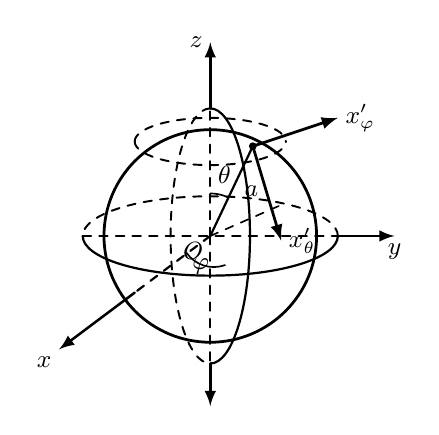
\begin{tikzpicture}[x=1.2cm, y=1.2cm, >=latex, line cap=round, line join=round]
    \draw[line width=1.0pt] (0, 0) circle (1.35cm);

    \draw[line width=0.8pt, dashed] (0, 0) -- (0, 1.35);
    \draw[line width=0.8pt, dashed] (0, 0) -- (0, -1.35);
    \draw[line width=0.9pt, ->] (0, 1.35) -- (0, 2.05) node[left=-1pt] {\small $z$};
    \draw[line width=0.9pt, ->] (0, -1.35) -- (0, -1.8);

    \draw[line width=0.8pt, dashed] (-1.35, 0) -- (1.35, 0);
    \draw[line width=0.9pt, ->] (1.35, 0) -- (1.95, 0) node[below=-1pt] {\small $y$};

    \draw[line width=0.8pt, dashed] (0, 0) -- (-0.8, -0.6);
    \draw[line width=0.9pt, ->] (-0.8, -0.6) -- (-1.6, -1.2) node[below left=-1pt] {\small $x$};
    \node[below left=-1pt] at (0, 0) {\small $O$};

    \draw[line width=0.7pt, dashed] (1.35, 0) arc[start angle=0, end angle=180, x radius=1.35, y radius=0.42];
    \draw[line width=0.8pt] (-1.35, 0) arc[start angle=180, end angle=360, x radius=1.35, y radius=0.42];

    \draw[line width=0.8pt] (0, 1.35) arc[start angle=90, end angle=-90, x radius=0.42, y radius=1.35];
    \draw[line width=0.7pt, dashed] (0, 1.35) arc[start angle=90, end angle=270, x radius=0.42, y radius=1.35];

    \draw[line width=0.7pt, dashed] (-0.8, 1.0) arc[start angle=180, end angle=360, x radius=0.8, y radius=0.25];
    \draw[line width=0.7pt, dashed] (-0.8, 1.0) arc[start angle=180, end angle=0, x radius=0.8, y radius=0.25];

    \coordinate (P) at (0.45, 0.95);
    \fill (P) circle (1.4pt);

    \draw[line width=0.8pt] (0, 0) -- (P) node[midway, right=1pt] {\small $a$};
    \draw[line width=0.6pt] (0, 0.45) arc[start angle=90, end angle=65, radius=0.45];
    \node at (0.15, 0.65) {\small $\theta$};

    \draw[line width=0.6pt, dashed] (0, 0) -- (0.8, 0.35);
    \draw[line width=0.6pt] (-0.25, -0.18) arc[start angle=215, end angle=290, radius=0.35];
    \node at (-0.1, -0.32) {\small $\varphi$};

    \draw[line width=1.0pt, ->] (P) -- ++(0.3, -1.0) node[right=-1pt] {\small $\boldsymbol{x}'_\theta$};
    \draw[line width=1.0pt, ->] (P) -- ++(0.9, 0.3) node[right=-1pt] {\small $\boldsymbol{x}'_\varphi$};
  \end{tikzpicture}
  \caption{}\label{fig:9.1.6}
\end{figure}

细心的读者会注意到 $\boldsymbol{x}'_{\theta} \times \boldsymbol{x}'_{\varphi} = F = 0$ 表明两个坐标切向量 $\boldsymbol{x}'_{\theta}$ 与 $\boldsymbol{x}'_{\varphi}$ 正交, 即 $\theta$ 线与 $\varphi$ 线为正交曲线网(\cref{fig:9.1.6}). \qedhere
\end{solution}

更一般地, 我们来求 $n - 1$ 维球面的单位法向量场.

\begin{example}\label{ex:9.1.11}
已知球心在坐标原点, 半径为 $a$ 的 $n - 1$ 维球面
\[
  S^{n-1}(a) = \left\{(x_{1}, x_{2}, \cdots, x_{n}) \in \mathbb{R}^{n} \mathrel{\Big|} \sum_{i=1}^{n}x_{i}^{2} = a^{2}\right\}, \quad a > 0.
\]
求 $n - 1$ 维球面 $S^{n-1}(a)$ 的单位法向量场、球面坐标及第一基本量.
\end{example}

\begin{solution}[解法 1]
令 $F(x_{1}, x_{2}, \cdots, x_{n}) = \sum_{i=1}^{n} x_{i}^{2} - a^{2}$, 则
\[
  F^{\prime}_{x_{i}} = 2x_{i}.
\]
因此, 单位法向量场为
\begin{align*}
  \boldsymbol{n}_{0} &= \pm\frac{1}{\sqrt{\sum_{i=1}^{n}(F_{x_{i}}^{\prime})^{2}}}(F_{x_{1}}^{\prime}, F_{x_{2}}^{\prime}, \cdots, F_{x_{n}}^{\prime}) = \pm\frac{1}{\sqrt{\sum_{i=1}^{n}(2x_{i})^{2}}}(2x_{1}, 2x_{2}, \cdots, 2x_{n}) \\
  &= \pm\left(\frac{x_{1}}{a}, \frac{x_{2}}{a}, \cdots, \frac{x_{n}}{a}\right).
\end{align*}
\end{solution}

\begin{solution}[解法 2]
设 $\boldsymbol{x}(\theta_{1}, \theta_{2}, \cdots, \theta_{n-1}) = (x_{1}(\theta_{1}, \cdots, \theta_{n-1}), x_{2}(\theta_{1}, \cdots, \theta_{n-1}), \cdots, x_{n}(\theta_{1}, \cdots, \theta_{n-1}))$, 其中
\[
  \left\{\begin{aligned}
    x_{1} &= a\cos\theta_{1}, \\
    x_{2} &= a\sin\theta_{1}\cos\theta_{2}, \\
    x_{3} &= a\sin\theta_{1}\sin\theta_{2}\cos\theta_{3}, \\
    &\;\;\vdots \\
    x_{n-1} &= a\sin\theta_{1}\sin\theta_{2}\sin\theta_{3}\cdots\sin\theta_{n-2}\cos\theta_{n-1}, \\
    x_{n} &= a\sin\theta_{1}\sin\theta_{2}\sin\theta_{3}\cdots\sin\theta_{n-2}\sin\theta_{n-1},
  \end{aligned}\right.
\]
而 $\theta_{1}, \theta_{2}, \cdots, \theta_{n-1}$ 称为球面参数, 也称为球面坐标. 不难验证第一基本量为
\[
  g_{ij} = \boldsymbol{x}^{\prime}_{\theta_{i}} \cdot \boldsymbol{x}^{\prime}_{\theta_{j}} = \left\{\begin{aligned}
    &0, && i \neq j, \\
    &a^{2}, && i = j = 1, \\
    &a^{2}\sin^{2}\theta_{1}\cdots\sin^{2}\theta_{i-1}, && i = j = 2, 3, \cdots, n - 1.
  \end{aligned}\right.
\]
由此得到 $\sqrt{\det(g_{ij})} = a^{n-1}\sin^{n-2}\theta_1\sin^{n-3}\theta_2\cdots\sin\theta_{n-2}$.

对 $\boldsymbol{x} \cdot \boldsymbol{x} = a^{2}$ 两边关于 $\theta_{i}$ 求偏导或直接对 $\boldsymbol{x}$ 关于 $\theta_{i}$ 求偏导验证得 $\boldsymbol{x} \cdot \dfrac{\partial\boldsymbol{x}}{\partial\theta_{i}} = 0$, $i = 1, 2, \cdots, n - 1$ 可知, $\boldsymbol{x}$ 为球面 $M$ 的法向量场. 因此, 单位法向量场为
\[
  \boldsymbol{n}_{0} = \pm\frac{\boldsymbol{x}}{\|\boldsymbol{x}\|} = \pm\frac{\boldsymbol{x}}{a} = \pm\left(\frac{x_{1}}{a}, \frac{x_{2}}{a}, \cdots, \frac{x_{n}}{a}\right). \qedhere
\]
\end{solution}

\begin{example}\label{ex:9.1.12}
{\emergencystretch=3em 从球面坐标, 平面极坐标 $(x_{1}, x_{2}) = (r \cos \theta, r \sin \theta)$ 以及三维 Euclid 空间 $\mathbb{R}^{3}$ 中的球坐标 $(x_{1}, x_{2}, x_{3}) = (r \cos \theta_{1}, r \sin \theta_{1} \cos \theta_{2}, r \sin \theta_{1} \sin \theta_{2})$ 或者 $(r \sin \theta \cos \varphi, r \sin \theta \sin \varphi, r \cos \theta)$(\cref{fig:9.1.7}), 自然会想到 $n$ 维 Euclid 空间 $\mathbb{R}^{n}$ 中应有球坐标.\par}

\begin{figure}[htbp]
  \centering
  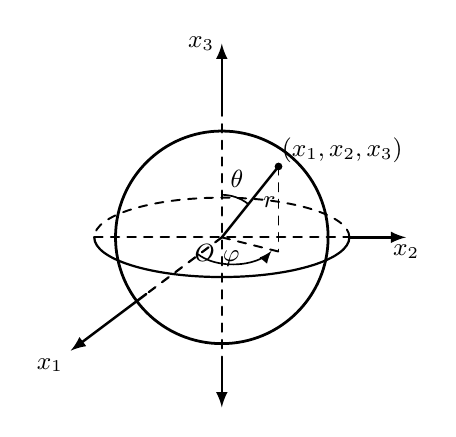
\begin{tikzpicture}[x=1.2cm, y=1.2cm, >=latex, line cap=round, line join=round]
    \draw[line width=1.0pt] (0, 0) circle (1.35cm);

    \draw[line width=0.8pt, dashed] (0, -1.35) -- (0, 1.35);
    \draw[line width=0.9pt, ->] (0, 1.35) -- (0, 2.05) node[left=-1pt] {\small $x_3$};
    \draw[line width=0.9pt, ->] (0, -1.35) -- (0, -1.8);

    \draw[line width=0.8pt, dashed] (-1.35, 0) -- (1.35, 0);
    \draw[line width=0.9pt, ->] (1.35, 0) -- (1.95, 0) node[below=-1pt] {\small $x_2$};

    \draw[line width=0.8pt, dashed] (0, 0) -- (-0.8, -0.6);
    \draw[line width=0.9pt, ->] (-0.8, -0.6) -- (-1.6, -1.2) node[below left=-1pt] {\small $x_1$};
    \node[below left=-1pt] at (0, 0) {\small $O$};

    \draw[line width=0.7pt, dashed] (1.35, 0) arc[start angle=0, end angle=180, x radius=1.35, y radius=0.42];
    \draw[line width=0.8pt] (-1.35, 0) arc[start angle=180, end angle=360, x radius=1.35, y radius=0.42];

    \coordinate (P) at (0.6, 0.75);
    \fill (P) circle (1.4pt) node[anchor=south west, inner sep=1pt] {\small $(x_1, x_2, x_3)$};

    \coordinate (Pxy) at (0.6, -0.15);
    \draw[line width=0.7pt, dashed] (P) -- (Pxy);
    \draw[line width=0.7pt, dashed] (0, 0) -- (Pxy);

    \draw[line width=0.9pt] (0, 0) -- (P) node[midway, right=1pt] {\small $r$};

    \draw[line width=0.6pt] (0, 0.45) arc[start angle=90, end angle=52, radius=0.45];
    \node at (0.16, 0.62) {\small $\theta$};

    \draw[line width=0.6pt, ->] (-0.25, -0.18) arc[start angle=215, end angle=335, x radius=0.45, y radius=0.25];
    \node at (0.1, -0.22) {\small $\varphi$};
  \end{tikzpicture}
  \caption{}\label{fig:9.1.7}
\end{figure}

$\boldsymbol{x}(r, \theta_{1}, \theta_{2}, \cdots, \theta_{n-1}) = (x_{1}(r, \theta_{1}, \cdots, \theta_{n-1}), x_{2}(r, \theta_{1}, \cdots, \theta_{n-1}), \cdots, x_{n}(r, \theta_{1}, \cdots, \theta_{n-1}))$ 为
\[
  \left\{\begin{aligned}
    x_{1} &= r\cos\theta_{1}, \\
    x_{2} &= r\sin\theta_{1}\cos\theta_{2}, \\
    x_{3} &= r\sin\theta_{1}\sin\theta_{2}\cos\theta_{3}, \\
    &\;\;\vdots \\
    x_{n-1} &= r\sin\theta_{1}\sin\theta_{2}\sin\theta_{3}\cdots\sin\theta_{n-2}\cos\theta_{n-1}, \\
    x_{n} &= r\sin\theta_{1}\sin\theta_{2}\sin\theta_{3}\cdots\sin\theta_{n-2}\sin\theta_{n-1},
  \end{aligned}\right.
\]
其中 $r, \theta_{1}, \theta_{2}, \cdots, \theta_{n-1}$ 为 $\mathbb{R}^{n}$ 的参数, 也称为球坐标. 不难验证第一基本量为
\[
  g_{00} = \boldsymbol{x}_{r}^{\prime} \cdot \boldsymbol{x}_{r}^{\prime} = 1,
\]
\[
  g_{0i} = \boldsymbol{x}_{r}^{\prime} \cdot \boldsymbol{x}_{\theta_{i}}^{\prime} = 0 = \boldsymbol{x}_{\theta_{i}}^{\prime} \cdot \boldsymbol{x}_{r}^{\prime} = g_{i0},
\]
\[
  g_{ij} = \left\{\begin{aligned}
    &0, && i \neq j, \\
    &r^{2}, && i = j = 1, \\
    &r^{2}\sin^{2}\theta_{1}\sin^{2}\theta_{2}\cdots\sin^{2}\theta_{i-1}, && i = j = 2, 3, \cdots, n - 1.
  \end{aligned}\right.
\]
由此得到
\begin{align*}
  \left(\frac{\partial(x_{1}, x_{2}, \cdots, x_{n})}{\partial(r, \theta_{1}, \theta_{2}, \cdots, \theta_{n-1})}\right)^{2}
  &= \det\begin{pmatrix}
    \dfrac{\partial x_{1}}{\partial r} & \cdots & \dfrac{\partial x_{n}}{\partial r} \\
    \dfrac{\partial x_{1}}{\partial\theta_{1}} & \cdots & \dfrac{\partial x_{n}}{\partial\theta_{1}} \\
    \vdots & & \vdots \\
    \dfrac{\partial x_{1}}{\partial\theta_{n-1}} & \cdots & \dfrac{\partial x_{n}}{\partial\theta_{n-1}}
  \end{pmatrix}\begin{pmatrix}
    \dfrac{\partial x_{1}}{\partial r} & \dfrac{\partial x_{1}}{\partial\theta_{1}} & \cdots & \dfrac{\partial x_{1}}{\partial\theta_{n-1}} \\
    \vdots & \vdots & & \vdots \\
    \dfrac{\partial x_{n}}{\partial r} & \dfrac{\partial x_{n}}{\partial\theta_{1}} & \cdots & \dfrac{\partial x_{n}}{\partial\theta_{n-1}}
  \end{pmatrix} \\
  &= \det\begin{pmatrix}
    g_{00} & g_{01} & \cdots & g_{0,n-1} \\
    g_{10} & g_{11} & \cdots & g_{1,n-1} \\
    \vdots & \vdots & & \vdots \\
    g_{n-1,0} & g_{n-1,1} & \cdots & g_{n-1,n-1}
  \end{pmatrix} \\
  &= \left[r^{n-1}\sin^{n-2}\theta_{1}\sin^{n-3}\theta_{2}\cdots\sin\theta_{n-2}\right]^{2}.
\end{align*}
如果注意到
\begin{align*}
  \frac{\partial(x_{1}, x_{2}, \cdots, x_{n})}{\partial(r, \theta_{1}, \theta_{2}, \cdots, \theta_{n-1})}\bigg|_{\left(r, \frac{\pi}{2}, \frac{\pi}{2}, \cdots, \frac{\pi}{2}\right)}
  &= \begin{vmatrix}
    0 & -r & 0 & \cdots & 0 \\
    0 & 0 & -r & \cdots & 0 \\
    \vdots & \vdots & \vdots & & \vdots \\
    0 & 0 & 0 & \cdots & -r \\
    1 & 0 & 0 & \cdots & 0
  \end{vmatrix} = (-1)^{1+n}(-r)^{n-1} \\
  &= r^{n-1} > 0,
\end{align*}
及直角坐标 $x_{1}, x_{2}, \cdots, x_{n}$ 与球坐标 $r, \theta_{1}, \theta_{2}, \cdots, \theta_{n-1}$ 之间变换的 Jacobi 行列式
\[
  \frac{\partial(x_{1}, x_{2}, \cdots, x_{n})}{\partial(r, \theta_{1}, \theta_{2}, \cdots, \theta_{n-1})}
\]
为连续函数, 它具有保号性, 因此有
\[
  \frac{\partial(x_{1}, x_{2}, \cdots, x_{n})}{\partial(r, \theta_{1}, \theta_{2}, \cdots, \theta_{n-1})} > 0.
\]
从而
\begin{align*}
  \frac{\partial(x_{1}, x_{2}, \cdots, x_{n})}{\partial(r, \theta_{1}, \theta_{2}, \cdots, \theta_{n-1})}
  &= \sqrt{\det\begin{pmatrix}
    g_{00} & g_{01} & \cdots & g_{0,n-1} \\
    g_{10} & g_{11} & \cdots & g_{1,n-1} \\
    \vdots & \vdots & & \vdots \\
    g_{n-1,0} & g_{n-1,1} & \cdots & g_{n-1,n-1}
  \end{pmatrix}} \\
  &= r^{n-1}\sin^{n-2}\theta_{1}\sin^{n-3}\theta_{2}\cdots\sin\theta_{n-2}.
\end{align*}
此行列式在应用 $n$ 元球坐标变换计算 $n$ 重积分时非常重要与简便.
\end{example}


\begin{example}\label{ex:9.1.13}
设 $U\subsetneq\mathbb{R}^{3}$ 为开集, $F, G\colon U \to \mathbb{R}^{1}$ 为两个三元函数,
\[
  L = \{(x, y, z) \in \mathbb{R}^{3} \mid F(x, y, z) = 0, \; G(x, y, z) = 0\},\quad
  \boldsymbol{x}^{0} = (x_{0}, y_{0}, z_{0}) \in L.
\]
如果 $F, G \in C^{k}(U, \mathbb{R}^{1})$, $k \geqslant 1$, 且 $\boldsymbol{x}^{0}$ 处的切向量
\[
  \boldsymbol{t}(\boldsymbol{x}^{0}) = \boldsymbol{J}\boldsymbol{F}(\boldsymbol{x}^{0}) \times
  \boldsymbol{J}\boldsymbol{G}(\boldsymbol{x}^{0}) =
  \begin{vmatrix}
    \boldsymbol{i} & \boldsymbol{j} & \boldsymbol{k} \\\\
    F_{x}^{\prime} & F_{y}^{\prime} & F_{z}^{\prime} \\\\
    G_{x}^{\prime} & G_{y}^{\prime} & G_{z}^{\prime}
  \end{vmatrix} \neq \boldsymbol{0},
\]
则 $\exists\,\boldsymbol{x}^{0}$ 的开邻域 $U_{0} \subset U$, s.\,t. $U_{0} \cap L$ 为一段 $C^{k}$ 参数曲线. 这时, $L$ 在 $\boldsymbol{x}^{0}$ 处的切线方程为
\[
  \left\{\begin{aligned}
    &F_{x}^{\prime}(\boldsymbol{x}^{0})(x - x_{0}) + F_{y}^{\prime}(\boldsymbol{x}^{0})(y - y_{0}) + F_{z}^{\prime}(\boldsymbol{x}^{0})(z - z_{0}) = 0, \\\\
    &G_{x}^{\prime}(\boldsymbol{x}^{0})(x - x_{0}) + G_{y}^{\prime}(\boldsymbol{x}^{0})(y - y_{0}) + G_{z}^{\prime}(\boldsymbol{x}^{0})(z - z_{0}) = 0.
  \end{aligned}\right.
\]

\begin{proof}
不妨设
\[
  \frac{\partial(F, G)}{\partial(y, z)}\bigg|_{\boldsymbol{x}^{0}} \neq 0.
\]
由隐函数定理, 存在含 $x_{0}$ 的开区间 $I$ 与含 $(y_{0}, z_{0})$ 的开区间 $J$ 使得方程组
\[
  F(x, y, z) = 0, \quad G(x, y, z) = 0
\]
在含 $\boldsymbol{x}^{0}$ 的开邻域 $U_{0} = I \times J$ 内有
\[
  y = f(x), \quad z = g(x), \quad x \in I,
\]
且 $f, g \in C^{k}(I, \mathbb{R}^{1})$. 因此, $U_{0} \cap L$ 为一段 $C^{k}$ 参数曲线
$\boldsymbol{x} = \boldsymbol{x}(x) = (x, f(x), g(x))$, $x$ 为其参数. 该曲线在 $\boldsymbol{x}^{0}$ 处的切向量为 $(1, f^{\prime}(x_{0}), g^{\prime}(x_{0}))$. 又因为
\[
  F(x, f(x), g(x)) \equiv 0, \quad G(x, f(x), g(x)) \equiv 0,
\]
所以
\[
  \left\{\begin{aligned}
    &F_{x}^{\prime} + F_{y}^{\prime}f^{\prime}(x) + F_{z}^{\prime}g^{\prime}(x) = 0, \\\\
    &G_{x}^{\prime} + G_{y}^{\prime}f^{\prime}(x) + G_{z}^{\prime}g^{\prime}(x) = 0,
  \end{aligned}\right.
\]
从而
\begin{align*}
  \bigl(1, f^{\prime}(x_{0}), g^{\prime}(x_{0})\bigr) \parallel \boldsymbol{t}(\boldsymbol{x}^{0})
  &= \bigl(F_{x}^{\prime}(\boldsymbol{x}^{0}), F_{y}^{\prime}(\boldsymbol{x}^{0}), F_{z}^{\prime}(\boldsymbol{x}^{0})\bigr)
     \times \bigl(G_{x}^{\prime}(\boldsymbol{x}^{0}), G_{y}^{\prime}(\boldsymbol{x}^{0}), G_{z}^{\prime}(\boldsymbol{x}^{0})\bigr) \\\\
  &= \boldsymbol{J}\boldsymbol{F}(\boldsymbol{x}^{0}) \times \boldsymbol{J}\boldsymbol{G}(\boldsymbol{x}^{0})
     \ (\text{图} \ \ref{fig:9.1.8}).
\end{align*}
\begin{figure}[htbp]
  \centering
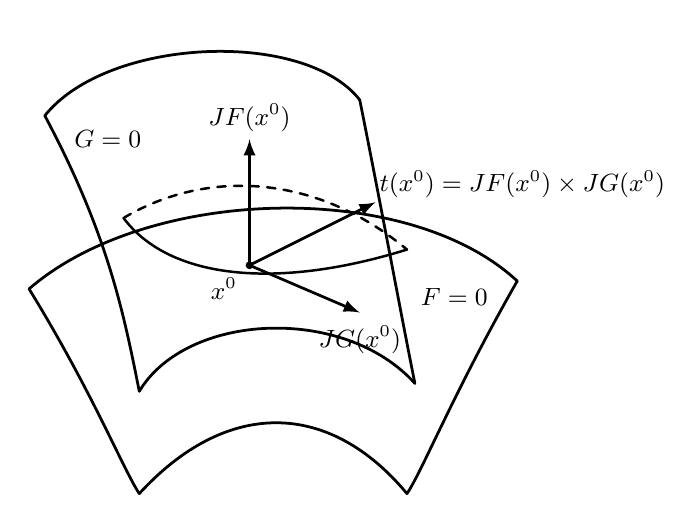
\begin{tikzpicture}[x=1.0cm, y=1.0cm, >=latex, line cap=round, line join=round]
    % 曲面 G=0 (后上)
    \draw[line width=1.0pt] (-2.8, 2.7) .. controls (-2.0, 3.7) and (0.5, 3.8) .. (1.2, 2.9);
    \draw[line width=1.0pt] (-2.8, 2.7) .. controls (-2.0, 1.2) and (-1.8, 0.2) .. (-1.6, -0.8);
    \draw[line width=1.0pt] (1.2, 2.9) .. controls (1.5, 1.4) and (1.7, 0.3) .. (1.9, -0.7);
    \draw[line width=1.0pt] (-1.6, -0.8) .. controls (-1.0, 0.2) and (1.0, 0.3) .. (1.9, -0.7);
    \node at (-2.0, 2.4) {\small $G = 0$};

    % 曲面 F=0 (横跨相交)
    \draw[line width=1.0pt] (-3.0, 0.5) .. controls (-1.5, 1.8) and (1.8, 1.9) .. (3.2, 0.6);
    \draw[line width=1.0pt] (-3.0, 0.5) .. controls (-2.2, -0.8) and (-1.8, -1.8) .. (-1.6, -2.1);
    \draw[line width=1.0pt] (3.2, 0.6) .. controls (2.4, -0.8) and (2.0, -1.8) .. (1.8, -2.1);
    \draw[line width=1.0pt] (-1.6, -2.1) .. controls (-0.5, -0.9) and (0.8, -0.9) .. (1.8, -2.1);
    \node at (2.4, 0.4) {\small $F = 0$};

    % 交线 (鞍形弧线，部分虚线)
    \draw[line width=0.9pt, dashed] (-1.8, 1.4) .. controls (-0.8, 2.0) and (0.6, 2.0) .. (1.8, 1.0);
    \draw[line width=0.9pt] (-1.8, 1.4) .. controls (-1.2, 0.6) and (0.2, 0.5) .. (1.8, 1.0);

    % 相交点 x^0
    \coordinate (X0) at (-0.2, 0.8);
    \fill (X0) circle (1.4pt) node[below left=1pt] {\small $\boldsymbol{x}^0$};

    % 法向量 JF 与 JG
    \draw[line width=1.0pt, ->] (X0) -- ++(0, 1.6) node[above=-1pt] {\small $\boldsymbol{J}F(\boldsymbol{x}^0)$};
    \draw[line width=1.0pt, ->] (X0) -- ++(1.4, -0.6) node[below=1pt] {\small $\boldsymbol{J}G(\boldsymbol{x}^0)$};

    % 切向量 t(x^0) = JF x JG
    \draw[line width=1.0pt, ->] (X0) -- ++(1.6, 0.8) node[anchor=south west, inner sep=1pt] {\small $\boldsymbol{t}(\boldsymbol{x}^0) = \boldsymbol{J}F(\boldsymbol{x}^0) \times \boldsymbol{J}G(\boldsymbol{x}^0)$};
  \end{tikzpicture}
  \caption{}\label{fig:9.1.8}
\end{figure}

由此知, 切线平行于 $\boldsymbol{t}(\boldsymbol{x}^{0})$, 而切线方程为
\[
  \left\{\begin{aligned}
    &F_{x}^{\prime}(\boldsymbol{x}^{0})(x - x_{0}) + F_{y}^{\prime}(\boldsymbol{x}^{0})(y - y_{0}) + F_{z}^{\prime}(\boldsymbol{x}^{0})(z - z_{0}) = 0, \\\\
    &G_{x}^{\prime}(\boldsymbol{x}^{0})(x - x_{0}) + G_{y}^{\prime}(\boldsymbol{x}^{0})(y - y_{0}) + G_{z}^{\prime}(\boldsymbol{x}^{0})(z - z_{0}) = 0.
  \end{aligned}\right.
\]
\qedhere
\end{proof}
\end{example}

\begin{example}\label{ex:9.1.14}
设 $\Delta \subset \mathbb{R}^{2}$ 为开区域, 曲面 $M$ 的参数表示为 $\boldsymbol{x}\colon \Delta \to \mathbb{R}^{3}$, 它是 $C^{1}$ 映射. 而 $(u(t), v(t))$ 对应于 $M$ 上的一条 $C^{1}$ 曲线, 其向量形式为
\[
  \boldsymbol{x} = \boldsymbol{x}(u(t), v(t)),
\]
\[
  \mathrm{d}\boldsymbol{x} = \bigl[\boldsymbol{x}_{u}^{\prime}u^{\prime}(t) + \boldsymbol{x}_{v}^{\prime}v^{\prime}(t)\bigr]\mathrm{d}t
  = \boldsymbol{x}_{u}^{\prime}\mathrm{d}u + \boldsymbol{x}_{v}^{\prime}\mathrm{d}v.
\]
弧元 $\mathrm{d}s$ 的平方为
\begin{align*}
  (\mathrm{d}s)^{2} &= (\mathrm{d}\boldsymbol{x})^{2} = \mathrm{d}\boldsymbol{x}\bullet\mathrm{d}\boldsymbol{x} \\\\
  &= \bigl[E{u^{\prime}}^{2}(t) + 2Fu^{\prime}(t)v^{\prime}(t) + G{v^{\prime}}^{2}(t)\bigr](\mathrm{d}t)^{2} \\\\
  &= E(\mathrm{d}u)^{2} + 2F\mathrm{d}u\mathrm{d}v + G(\mathrm{d}v)^{2}.
\end{align*}
由此得到 $M$ 上从点 $\boldsymbol{x}(u(\alpha), v(\alpha))$ 到 $\boldsymbol{x}(u(\beta), v(\beta))$ 的曲线的弧长为
\[
  s = \int_{\alpha}^{\beta}\sqrt{E\,{u^{\prime}}^{2}(t) + 2Fu^{\prime}(t)v^{\prime}(t) + G\,{v^{\prime}}^{2}(t)}\;\mathrm{d}t.
\]
考虑例 \ref{ex:9.1.10} 中的球面 $M$ 上的两点 $p$ 与 $q$. 不失一般性, 可设 $p$ 与 $q$ 在 $M$ 的同一条经线上. 设这两点的参数分别为 $(\theta_{0}, \varphi_{0})$ 与 $(\theta_{1}, \varphi_{1})$, 其中 $\theta_{1} > \theta_{0}$. 这两点所决定的球面曲线记为 $\Gamma$, 其 $C^{1}$ 参数表示为
\[
  \bigl(\theta(t), \varphi(t)\bigr), \quad t_{0} \leqslant t \leqslant t_{1}.
\]
于是, $\Gamma$ 的弧长为
\begin{align*}
  s(\Gamma) &= \int_{t_{0}}^{t_{1}}\sqrt{a^{2}\bigl[\theta^{\prime}(t)\bigr]^{2} + a^{2}\sin^{2}\theta(t) \cdot \bigl[\varphi^{\prime}(t)\bigr]^{2}}\;\mathrm{d}t \\\\
  &\geqslant a\int_{t_{0}}^{t_{1}}\theta^{\prime}(t)\mathrm{d}\theta
  = a\bigl[\theta(t_{1}) - \theta(t_{0})\bigr].
\end{align*}
式中等号成立等价于 $\varphi^{\prime}(t) = \vec{0}$ 等价于 $\varphi(t) = \varphi_{0}$ (常值). 这时曲线 $\Gamma$ 正是由 $p$ 与 $q$ 两点所决定的大圆弧, 而
$  a\bigl[\theta(t_{1}) - \theta(t_{0})\bigr] = a(\theta_{1} - \theta_{0})$ 恰为这一段大圆弧的弧长.
\end{example}

\begin{definition}\label{def:9.1.4}
设 $s$ 维 $C^{k}\,(k \geqslant 1)$ 正则曲面 $M$ 的参数表示为 $\boldsymbol{x}(u_{1}, u_{2}, \cdots, u_{s})$, 它的第一基本量为
\[
  g_{ij} = \boldsymbol{x}_{u_{i}}^{\prime} \cdot \boldsymbol{x}_{u_{j}}^{\prime}, \quad i, j = 1, 2, \cdots, s.
\]
我们称
\[
  I = \sum_{i, j = 1}^{s}g_{ij}\mathrm{d}u_{i}\mathrm{d}u_{j}
\]
为曲面 $M$ 或 $\boldsymbol{x}(\boldsymbol{u})$ 的第一基本形式. 易见,
\begin{align*}
  (\mathrm{d}\boldsymbol{x})^{2} &= \mathrm{d}\boldsymbol{x}\bullet\mathrm{d}\boldsymbol{x} \\\\
  &= \Bigl(\sum_{i=1}^{s}\boldsymbol{x}_{u_{i}}^{\prime}\mathrm{d}u_{i}\Bigr)
     \bullet \Bigl(\sum_{j=1}^{s}\boldsymbol{x}_{u_{j}}^{\prime}\mathrm{d}u_{j}\Bigr) \\\\
  &= \sum_{i, j = 1}^{s}\boldsymbol{x}_{u_{i}}^{\prime}\bullet\boldsymbol{x}_{u_{j}}^{\prime}\mathrm{d}u_{i}\mathrm{d}u_{j}
  = \sum_{i, j = 1}^{s}g_{ij}\mathrm{d}u_{i}\mathrm{d}u_{j} = I.
\end{align*}
考察 $M$ 上的曲线 $\boldsymbol{u}(t)$ 或 $\boldsymbol{x}(\boldsymbol{u}(t))$, 则弧元 $\mathrm{d}s$ 的平方为
\begin{align*}
  (\mathrm{d}s)^{2} &= (\mathrm{d}\boldsymbol{x})^{2} = \mathrm{d}\boldsymbol{x}\cdot\mathrm{d}\boldsymbol{x} \\\\
  &= \Bigl(\sum_{i=1}^{s}\boldsymbol{x}_{u_{i}}^{\prime}\mathrm{d}u_{i}\Bigr)
     \cdot \Bigl(\sum_{j=1}^{s}\boldsymbol{x}_{u_{j}}^{\prime}\mathrm{d}u_{j}\Bigr) \\\\
  &= \sum_{i, j = 1}^{s}\boldsymbol{x}_{u_{i}}^{\prime}\cdot\boldsymbol{x}_{u_{j}}^{\prime}\mathrm{d}u_{i}\mathrm{d}u_{j}
  = \sum_{i, j = 1}^{s}g_{ij}\mathrm{d}u_{i}\mathrm{d}u_{j},
\end{align*}
其中 $\mathrm{d}u_{i} = \mathrm{d}u_{i}(t) = u_{i}^{\prime}(t)\mathrm{d}t$. 从 $t_{0}$ 到 $t_{1}$ 相应的弧长为
\[
  s\bigg|_{t_{0}}^{t_{1}} = \int_{t_{0}}^{t_{1}}\sqrt{\sum_{i, j = 1}^{s}g_{ij}u_{i}^{\prime}u_{j}^{\prime}}\;\mathrm{d}t.
\]
当 $s = 2$ 时, $g_{11} = E$, $g_{12} = g_{21} = F$, $g_{22} = G$, 由 $\boldsymbol{x}_{u}^{\prime}\mathrm{d}u$ 与 $\boldsymbol{x}_{v}^{\prime}\mathrm{d}v$ 张成的平行四边形的面积
\begin{align*}
  \mathrm{d}\boldsymbol{\sigma} &= \bigl\lVert\boldsymbol{x}_{u}^{\prime}\mathrm{d}u \times \boldsymbol{x}_{v}^{\prime}\mathrm{d}v\bigr\rVert
  = \bigl\lVert\boldsymbol{x}_{u}^{\prime} \times \boldsymbol{x}_{v}^{\prime}\bigr\rVert\mathrm{d}u\mathrm{d}v \\\\
  &= \sqrt{EG - F^{2}}\;\mathrm{d}u\mathrm{d}v
\end{align*}
称为该曲面的面积元, 也称为二维体积元(图 \ref{fig:9.1.9}).

\begin{figure}[htbp]
  \centering
\begin{tikzpicture}[x=1.0cm, y=1.0cm, >=latex, line cap=round, line join=round]
    % 曲面 M
    \draw[line width=1.0pt] (-0.2, 2.0) .. controls (1.0, 2.8) and (3.0, 2.8) .. (4.0, 1.6);
    \draw[line width=1.0pt] (-0.2, 2.0) .. controls (0.6, 1.4) and (1.4, 1.5) .. (2.2, 0.8)
                            .. controls (3.0, 1.1) and (3.6, 1.2) .. (4.0, 1.6);
    \node at (3.8, 1.2) {\small $M$};

    \coordinate (XUV) at (1.5, 1.8);

    % 参数网格虚线
    \draw[line width=0.8pt, dashed] (0.3, 1.4) .. controls (1.0, 2.0) and (1.5, 2.3) .. (3.4, 2.3);
    \draw[line width=0.8pt] (0.8, 2.5) .. controls (1.3, 2.0) and (2.0, 1.5) .. (2.7, 0.8);

    % 切平面 (平行四边形外框)
    \coordinate (TP1) at (0.5, 1.8);
    \coordinate (TP2) at (1.6, 3.2);
    \coordinate (TP3) at (3.5, 2.6);
    \coordinate (TP4) at (2.4, 1.2);
    \draw[line width=0.8pt] (TP1) -- (TP2) -- (TP3) -- (TP4) -- cycle;

    % 微元面积平行四边形 (带阴影)
    \coordinate (DP1) at (XUV);
    \coordinate (DP2) at ($(XUV) + (0.3, 1.1)$);
    \coordinate (DP3) at ($(XUV) + (1.5, 1.15)$);
    \coordinate (DP4) at ($(XUV) + (1.2, 0.05)$);

    \fill[pattern=north east lines, pattern color=black!70] (DP1) -- (DP2) -- (DP3) -- (DP4) -- cycle;
    \draw[line width=0.9pt] (DP1) -- (DP2) -- (DP3) -- (DP4) -- cycle;

    % 微元边向量
    \draw[line width=1.0pt, ->] (DP1) -- (DP4) node[right=-1pt] {\small $\boldsymbol{x}'_u \mathrm{d}u$};
    \draw[line width=1.0pt, ->] (DP1) -- (DP2) node[above=-1pt] {\small $\boldsymbol{x}'_v \mathrm{d}v$};

    \fill (XUV) circle (1.4pt) node[below=2pt] {\small $\boldsymbol{x}(u,v)$};
  \end{tikzpicture}
  \caption{}\label{fig:9.1.9}
\end{figure}

更一般地, 由 $\boldsymbol{x}_{u_{i}}^{\prime}\mathrm{d}u_{i}$, $i = 1, 2, \cdots, s$ 张成的 $s$ 维平行 $2s$ 面体的体积
\[
  \mathrm{d}\sigma = \sqrt{\det(g_{ij})}\;\mathrm{d}u_{1}\mathrm{d}u_{2}\cdots\mathrm{d}u_{s}
\]
称为该 $s$ 维曲面的 $s$ 维体积元.
\end{definition}

\begin{example}\label{ex:9.1.15}
求下列曲面的第一基本形式及体积元:

(1) $\mathbb{R}^{3}$ 中二维曲面 $M$, 参数表示为 $\boldsymbol{x}(x, y) = (x, y, z(x, y))$, $z(x, y)$ 为 $C^{1}$ 函数;

(2) $\mathbb{R}^{3}$ 中二维球面 $S^{2}(a)$, 参数表示为
$\boldsymbol{x}(\theta, \varphi) = (a\sin\theta\cos\varphi, a\sin\theta\sin\varphi, a\cos\theta)$, $a > 0$;

(3) $\mathbb{R}^{n}$ 中 $n-1$ 维球面 $S^{n-1}(a)$, 参数表示 $\boldsymbol{x}(\theta_{1}, \theta_{2}, \cdots, \theta_{n-1})$, 如例 \ref{ex:9.1.11} 所示;

(4) $\mathbb{R}^{n}$ 中 $n$ 维参数曲面 $\boldsymbol{x}(r, \theta_{1}, \theta_{2}, \cdots, \theta_{n-1})$, 如例 \ref{ex:9.1.12} 所示.

\begin{solution}
(1) 因为
\[
  \boldsymbol{x}_{x}^{\prime} = (1, 0, z_{x}^{\prime}), \quad \boldsymbol{x}_{y}^{\prime} = (0, 1, z_{y}^{\prime}),
\]
\[
  \begin{pmatrix} g_{11} & g_{12} \\ g_{21} & g_{22} \end{pmatrix}
  = \begin{pmatrix} E & F \\ F & G \end{pmatrix}
  = \begin{pmatrix} 1 + {z^{\prime}}_{x}^{2} & z_{x}^{\prime}z_{y}^{\prime} \\ z_{x}^{\prime}z_{y}^{\prime} & 1 + {z^{\prime}}_{y}^{2} \end{pmatrix},
\]
所以, 曲面 $M$ 的第一基本形式为
\begin{align*}
  I &= E(\mathrm{d}x)^{2} + 2F\mathrm{d}x\mathrm{d}y + G(\mathrm{d}y)^{2} \\\\
  &= (1 + {z_{x}^{\prime}}^{2})(\mathrm{d}x)^{2} + 2z_{x}^{\prime}z_{y}^{\prime}\mathrm{d}x\mathrm{d}y
     + (1 + {z_{y}^{\prime}}^{2})(\mathrm{d}y)^{2}. \qedhere
\end{align*}
而面积元为
\begin{align*}
  \mathrm{d}\sigma &= \sqrt{EG - F^{2}}\;\mathrm{d}x\mathrm{d}y \\\\
  &= \sqrt{(1 + {z_{x}^{\prime}}^{2})(1 + {z_{y}^{\prime}}^{2}) - (z_{x}^{\prime}z_{y}^{\prime})^{2}}\;\mathrm{d}x\mathrm{d}y \\\\
  &= \sqrt{1 + {z_{x}^{\prime}}^{2} + {z_{y}^{\prime}}^{2}}\;\mathrm{d}x\mathrm{d}y.
\end{align*}

(2) 由例 \ref{ex:9.1.10} 解法 2 知, 二维球面 $M$ 的第一基本形式为
\[
  I = a^{2}(\mathrm{d}\theta)^{2} + a^{2}\sin^{2}\theta(\mathrm{d}\varphi)^{2}.
\]
而面积元为
\[
  \mathrm{d}\sigma = \sqrt{EG - F^{2}}\;\mathrm{d}\theta\mathrm{d}\varphi = a^{2}\sin\theta\;\mathrm{d}\theta\mathrm{d}\varphi.
\]

(3) 由例 \ref{ex:9.1.11} 的解法 2 知, $n-1$ 维球面 $S^{n-1}(a)$ 的第一基本形式为
\begin{align*}
  I &= a^{2}(\mathrm{d}\theta_{1})^{2} + a^{2}\sin^{2}\theta_{1}(\mathrm{d}\theta_{2})^{2} + \cdots
     + a^{2}\sin^{2}\theta_{1}\cdots\sin^{2}\theta_{i-1}(\mathrm{d}\theta_{i})^{2} \\\\
  &\quad + \cdots + a^{2}\sin^{2}\theta_{1}\cdots\sin^{2}\theta_{n-2}(\mathrm{d}\theta_{n-1})^{2}.
\end{align*}
而面积元为
\begin{align*}
  \mathrm{d}\sigma &= \sqrt{\det(g_{ij})}\;\mathrm{d}\theta_{i}\mathrm{d}\theta_{i+1}\cdots\mathrm{d}\theta_{n-1} \\\\
  &= a^{n-1}\sin^{n-2}\theta_{1}\sin^{n-3}\theta_{2}\cdots\sin^{2}\theta_{n-3}\sin\theta_{n-2}
     \;\mathrm{d}\theta_{1}\mathrm{d}\theta_{2}\cdots\mathrm{d}\theta_{n-1}.
\end{align*}

(4) 由例 \ref{ex:9.1.12} 知, $\boldsymbol{x}(r, \theta_{1}, \theta_{2}, \cdots, \theta_{n-1})$ 的第二基本形式为(原文如此)
\begin{align*}
  I &= \mathrm{d}r^{2} + r^{2}(\mathrm{d}\theta_{1})^{2} + r^{2}\sin^{2}\theta_{1}(\mathrm{d}\theta_{2})^{2} + \cdots \\\\
  &\quad + r^{2}\sin^{2}\theta_{1}\cdots\sin^{2}\theta_{i-1}(\mathrm{d}\theta_{i})^{2}
  + \cdots + r^{2}\sin^{2}\theta_{1}\cdots\sin^{2}\theta_{n-2}(\mathrm{d}\theta_{n-1})^{2}.
\end{align*}
而体积元为
\begin{align*}
  \mathrm{d}v &= \sqrt{\det(g_{ij})}\;\mathrm{d}r\mathrm{d}\theta_{1}\mathrm{d}\theta_{2}\cdots\mathrm{d}\theta_{n-1} \\\\
  &= r^{n-1}\sin^{n-2}\theta_{1}\sin^{n-3}\theta_{2}\cdots\sin^{2}\theta_{n-3}\sin\theta_{n-2}
     \;\mathrm{d}r\mathrm{d}\theta_{1}\mathrm{d}\theta_{2}\cdots\mathrm{d}\theta_{n-1}. \qedhere
\end{align*}
\end{solution}
\end{example}

\begin{exblock}{练习题 9.1}
  \item 求下列曲面在指定点处的法向量, 切平面方程与法线方程:

  (1) $x^{2} + y^{2} + z^{2} = 4$, $\boldsymbol{x}^{0} = \left(1, 1, \sqrt{2}\right)$;

  (2) $z = \arctan \dfrac{y}{x}$, $\boldsymbol{x}^{0} = \left(1, 1, \dfrac{\pi}{4}\right)$;

  (3) $3x^{2} + 2y^{2} - 2z - 1 = 0$, $\boldsymbol{x}^{0} = (1, 1, 2)$;

  (4) $z = y + \ln\left(\dfrac{x}{z}\right)$, $\boldsymbol{x}^{0} = (1, 1, 1)$;

  (5) $y - \mathrm{e}^{2x - z} = 0$, $\dot{\boldsymbol{x}}^{0} = (1, 1, 2)$;

  (6) $\dfrac{x^{2}}{a^{2}} + \dfrac{y^{2}}{b^{2}} + \dfrac{z^{2}}{c^{2}} = 1$,
  $\boldsymbol{x}^{0} = \left(\dfrac{a}{\sqrt{3}}, \dfrac{b}{\sqrt{3}}, \dfrac{c}{\sqrt{3}}\right)$.

  \item 求椭球面 $x^{2} + 2y^{2} + 3z^{2} = 21$ 上所有平行于平面 $x + 4y + 6z = 0$ 的切平面.

  \item 求曲面 $x^{2} + y^{2} + z^{2} = x$ 的切平面, 使其垂直于平面 $x - y - z = 2$ 与 $x - y - \dfrac{z}{2} = 2$.

  \item 求两曲面
  \[ F(x, y, z) = 0, \quad G(x, y, z) = 0 \]
  的交线在 $xOy$ 平面上的投影曲线的切线方程, 并给出求切线方程的条件.

  \item 两相交曲面在交点处的法向量所夹的角称为这两曲面在这一点的夹角. 求圆柱面 $x^{2} + y^{2} = a^{2}$ 与曲面 $bz = xy$ 的夹角.

  \item 求椭球面
  \[ \frac{x^{2}}{a^{2}} + \frac{y^{2}}{b^{2}} + \frac{z^{2}}{c^{2}} = 1 \]
  上的点的法向量与 $x$ 轴和 $z$ 轴夹成等角的点的全体.

  \item 定出正数 $\lambda$, 使曲面 $xyz = \lambda$ 与椭球面
  \[ \frac{x^{2}}{a^{2}} + \frac{y^{2}}{b^{2}} + \frac{z^{2}}{c^{2}} = 1 \]
  在某一点相切, 即有共同的切平面.

  \item 证明: 曲面 $z = x\mathrm{e}^{\frac{x}{y}}$ 上所有切平面都通过原点.

  \item 证明: 曲面 $\sqrt{x} + \sqrt{y} + \sqrt{z} = \sqrt{a}\,(a > 0)$ 的切平面在各坐标平面上割下的诸线段之和为常数.

  \item 证明: 曲面 $F(x - az, y - bz) = 0$ 的所有切平面与某一直线平行, 其中 $a$, $b$ 为常数. 并说明论述中需加什么条件.

  \item 证明: 曲面 $F\left(\dfrac{x-a}{z-c}, \dfrac{y-b}{z-c}\right) = 0$ 的切平面通过一个固定点, 其中 $a$, $b$, $c$ 为常数. 并说明论述中需加什么条件.

  \item 证明: 曲面 $ax + by + cz = \Phi(x^{2} + y^{2} + z^{2})$ 在点 $\boldsymbol{x}^{0} = (x_{0}, y_{0}, z_{0})$ 处的法向量与向量 $(x_{0}, y_{0}, z_{0})$ 和 $(a, b, c)$ 共面. 并说明论述中需加什么条件.

  \item 求下列曲面的 $E$, $F$ 与 $G$, 第一基本形式及面积元:

  (1) 椭球面 $\boldsymbol{x}(u, v) = (a\sin u\cos v, b\sin u\sin v, c\cos u)$;

  (2) 单叶双曲面 $\boldsymbol{x}(u, v) = (a\,\mathrm{ch}\,u\cos v, b\,\mathrm{ch}\,u\sin v, c\,\mathrm{sh}\,u)$;

  (3) 椭圆抛物面 $\boldsymbol{x}(u, v) = \left(u, v, \dfrac{1}{2}\left(\dfrac{u^{2}}{a^{2}} + \dfrac{v^{2}}{b^{2}}\right)\right)$;

  (4) 双曲抛物面 $\boldsymbol{x}(u, v) = (a(u + v), b(u - v), 2uv)$;

  (5) 劈锥面 $\boldsymbol{x}(u, v) = (u\cos v, u\sin v, \varphi(v))$;

  (6) 一般螺面 $\boldsymbol{x}(u, v) = (u\cos v, u\sin v, \varphi(u) + av)$.

  \item 求 $\mathbb{R}^{3}$ 中圆柱面 $\boldsymbol{x}(\theta, z) = (a\cos\theta, a\sin\theta, z)$ 的第一基本形式与面积元.

  \item 设曲面 $M$ 的第一基本形式为
  \[ I = \mathrm{d}u^{2} + (u^{2} + a^{2})\mathrm{d}v^{2}, \]
  求曲面上的曲线 $u = v$ 从 $v_{1}$ 到 $v_{2}\,(> v_{1})$ 这一段的弧长.

  \item 求平面曲线(星形线) $x^{\frac{2}{3}} + y^{\frac{2}{3}} = a^{\frac{2}{3}}\,(a > 0)$ 上任一点处的切线方程, 并证明这些切线被坐标轴所截取的线段等长(应用 $F(x, y) = x^{\frac{2}{3}} + y^{\frac{2}{3}} - a^{\frac{2}{3}} = 0$ 与参数表示 $(x, y) = (a\cos^{3}t, a\sin^{3}t)$ 两种方法求曲线的切向量).

  \item 求下列曲线所示点处的切线与法平面:

  (1) $(x, y, z) = (a\sin^{2}t, b\sin t\cos t, c\cos^{2}t)$, 在点 $t = \dfrac{\pi}{4}$;

  (2) $2x^{2} + 3y^{2} + z^{2} = 9$, $z^{2} = 3x^{2} + y^{2}$, 在点 $(1, -1, -2)$.

  \item 证明: 球面 $x^{2} + y^{2} + z^{2} = \rho^{2}$ 与锥面 $x^{2} + y^{2} = z^{2}\tan^{2}\varphi$ 是正交的($\rho > 0$ 与 $\varphi$ 为常数).

  \item 在曲线 $(x, y, z) = (t, t^{2}, t^{3})$ 上求出一点, 使曲线在此点的切线平行于平面 $x + 2y + z = 4$.

  \item 求函数
  \[ u = \frac{x}{\sqrt{x^{2} + y^{2} + z^{2}}} \]
  沿曲线 $(x, y, z) = (t, 2t^{2}, -2t^{4})$ 在点 $(1, 2, -2)$ 处切线方向的方向导数.

  \item {\emergencystretch=3em 设 $(x_{0}, y_{0}, z_{0})$ 为曲面 $F(x, y, z) = 1$ 的非奇异点(若
  $\bigl(F_{x}^{\prime}(x_{0}, y_{0}, z_{0}),\allowbreak F_{y}^{\prime}(x_{0}, y_{0}, z_{0}),\allowbreak F_{z}^{\prime}(x_{0}, y_{0}, z_{0})\bigr) \neq (0, 0, 0)$, 则称 $(x_{0}, y_{0}, z_{0})$ 为非奇异点; 否则 $(x_{0}, y_{0}, z_{0})$ 称为奇异点), $F$ 在 $(x_{0}, y_{0}, z_{0})$ 的开邻域 $U$ 内可微, 且为 $n$ 次齐次函数. 证明: 曲面在 $(x_{0}, y_{0}, z_{0})$ 处的切平面方程为\par}
  \[
    xF_{x}^{\prime}(x_{0}, y_{0}, z_{0}) + yF_{y}^{\prime}(x_{0}, y_{0}, z_{0})
    + zF_{z}^{\prime}(x_{0}, y_{0}, z_{0}) = n.
  \]

  \item 设 $F(u, v)$ 为 $C^{1}$ 函数, 证明: 曲面 $F(nx - lz, ny - mz) = 0$ 上任一点的切平面都平行于直线 $L\colon \dfrac{x}{l} = \dfrac{y}{m} = \dfrac{z}{n}$.

  \item 从原点向单叶双曲面
  \[ \frac{x^{2}}{a^{2}} + \frac{y^{2}}{b^{2}} - \frac{z^{2}}{c^{2}} = 1 \]
  的切平面引垂线, 求垂足的轨迹.

  \item 设 $a > 0$, $b > 0$, $c > 0$. 证明: $\mathbb{R}^{3}$ 中任意一点 $(x, y, z)$ 处, 有三个彼此正交的二次曲面
  \[ \frac{x^{2}}{a^{2} - \lambda_{i}^{2}} + \frac{y^{2}}{b^{2} - \lambda_{i}^{2}} + \frac{z^{2}}{c^{2} - \lambda_{i}^{2}} = -1, \quad i = 1, 2, 3, \]
  其中 $\lambda_{1}, \lambda_{2}, \lambda_{3}$ 为三个彼此不同的实数.
\end{exblock}


\section{$n$ 元函数的极值与最值}\label{sec:9.2}

在第一册中, 我们学习过一元函数的极值与最值, 在这一节中将把这些概念与方法推广到 $n$ 元函数中去.

\begin{definition}\label{def:9.2.1}
设 $D \subset \mathbb{R}^{n}$ 为开集, $f\colon D \to \mathbb{R}^{1}$ 为 $n$ 元函数, $\boldsymbol{x}^{0} \in D$. 若存在 $\boldsymbol{x}^{0}$ 的开邻域 $U \subset D$, 使得对于 $\forall \boldsymbol{x} \in U \setminus \{\boldsymbol{x}^{0}\}$, 都有
\[
  f(\boldsymbol{x}) \leqslant f(\boldsymbol{x}^{0}) \quad (\text{或 } f(\boldsymbol{x}) \geqslant f(\boldsymbol{x}^{0})),
\]
则称 $f$ 在 $\boldsymbol{x}^{0}$ 取\textbf{极大值}(或\textbf{极小值}), 相应的点 $\boldsymbol{x}^{0}$ 称为 $f$ 的\textbf{极大值点}(或\textbf{极小值点}). 极大值与极小值统称为\textbf{极值}, 极大值点与极小值点统称为\textbf{极值点}.

如果对于 $\forall \boldsymbol{x} \in U \setminus \{\boldsymbol{x}^{0}\}$, 都有严格不等式
\[
  f(\boldsymbol{x}) < f(\boldsymbol{x}^{0}) \quad (\text{或 } f(\boldsymbol{x}) > f(\boldsymbol{x}^{0})),
\]
则称 $f$ 在 $\boldsymbol{x}^{0}$ 取\textbf{严格极大值}(或\textbf{严格极小值}), 点 $\boldsymbol{x}^{0}$ 称为 $f$ 的\textbf{严格极大值点}(或\textbf{严格极小值点}).
\end{definition}

从一元函数的知识知道, 若 $f(x)$ 在 $x_{0}$ 处取得极值, 且 $f'(x_{0})$ 存在, 则必有 $f'(x_{0}) = 0$. 这个结论对多元函数也是成立的.

\begin{theorem}[极值的必要条件]\label{thm:9.2.1}
设 $D \subset \mathbb{R}^{n}$ 为开集, $f\colon D \to \mathbb{R}^{1}$ 为 $n$ 元函数, $\boldsymbol{x}^{0} \in D$ 为 $f$ 的极值点. 若偏导数 $\dfrac{\partial f}{\partial x_{i}}(\boldsymbol{x}^{0})$ ($i = 1, 2, \cdots, n$) 存在, 则必有
\[
  \frac{\partial f}{\partial x_{i}}(\boldsymbol{x}^{0}) = 0 \quad (i = 1, 2, \cdots, n).
\]
即 $\operatorname{grad}f(\boldsymbol{x}^{0}) = \boldsymbol{0}$.
\end{theorem}

\begin{proof}
不妨设 $\boldsymbol{x}^{0}$ 为 $f$ 的极大值点. 于是存在 $\boldsymbol{x}^{0}$ 的球形开邻域 $B(\boldsymbol{x}^{0}, \delta) \subset D$, 使得对于 $\forall \boldsymbol{x} \in B(\boldsymbol{x}^{0}, \delta)$, 都有
\[
  f(\boldsymbol{x}) \leqslant f(\boldsymbol{x}^{0}).
\]
固定其余变量 $x_{j} = x_{j}^{0}$ ($j \neq i$), 令 $x_{i} \in (x_{i}^{0} - \delta, x_{i}^{0} + \delta)$, 考查一元函数
\[
  g_{i}(x_{i}) = f(x_{1}^{0}, \cdots, x_{i-1}^{0}, x_{i}, x_{i+1}^{0}, \cdots, x_{n}^{0}).
\]
显然, $g_{i}(x_{i})$ 在区间 $(x_{i}^{0} - \delta, x_{i}^{0} + \delta)$ 内于点 $x_{i}^{0}$ 处取得极大值. 又因为偏导数 $\dfrac{\partial f}{\partial x_{i}}(\boldsymbol{x}^{0})$ 存在, 所以一元函数导数 $g_{i}'(x_{i}^{0})$ 存在, 且 $g_{i}'(x_{i}^{0}) = \dfrac{\partial f}{\partial x_{i}}(\boldsymbol{x}^{0})$. 根据一元函数极值的必要条件(Fermat 定理), 必有
\[
  g_{i}'(x_{i}^{0}) = \frac{\partial f}{\partial x_{i}}(\boldsymbol{x}^{0}) = 0 \quad (i = 1, 2, \cdots, n).
\]
这就证明了 $\operatorname{grad}f(\boldsymbol{x}^{0}) = \boldsymbol{0}$.
\end{proof}

满足 $\operatorname{grad}f(\boldsymbol{x}^{0}) = \boldsymbol{0}$ 的点 $\boldsymbol{x}^{0}$ 称为函数 $f$ 的\textbf{驻点}(或\textbf{稳定点}). 定理 \ref{thm:9.2.1} 表明: 可微函数的极值点必为驻点. 但反过来, 驻点不一定是极值点, 例如函数 $f(x, y) = xy$, 在原点 $(0, 0)$ 处显然有 $f_{x}'(0, 0) = 0$, $f_{y}'(0, 0) = 0$, 所以 $(0, 0)$ 为驻点. 但是在原点的任何开邻域内, 都有点使得 $f(x, y) > 0$ (第一、三象限), 也有点使得 $f(x, y) < 0$ (第二、四象限), 而 $f(0, 0) = 0$, 故 $(0, 0)$ 不是极值点(此点称为鞍点).

因此, 驻点只是极值的必要条件, 还必须寻求极值的充分条件.

回忆一元函数 $f(x)$ 极值的充分条件: 若 $f'(x_{0}) = 0$, 且 $f''(x_{0})$ 存在, 则当 $f''(x_{0}) > 0$ 时, $x_{0}$ 为严格极小值点; 当 $f''(x_{0}) < 0$ 时, $x_{0}$ 为严格极大值点. 对于多元函数, 二阶导数由 Hesse 矩阵代替.

设 $f\colon D \to \mathbb{R}^{1}$ 具有二阶连续偏导数, 即 $f \in C^{2}(D, \mathbb{R}^{1})$, 则 $f$ 在点 $\boldsymbol{x}^{0}$ 处的 Hesse 矩阵为
\[
  \boldsymbol{H}f(\boldsymbol{x}^{0}) = \left(\frac{\partial^{2}f}{\partial x_{i}\partial x_{j}}(\boldsymbol{x}^{0})\right)_{n \times n}.
\]
由 Schwarz 定理知, $\boldsymbol{H}f(\boldsymbol{x}^{0})$ 为实对称矩阵. 二次型
\[
  Q(\boldsymbol{h}) = \boldsymbol{h} \boldsymbol{H}f(\boldsymbol{x}^{0}) \boldsymbol{h}^{\mathrm{T}} = \sum_{i,j=1}^{n} \frac{\partial^{2}f}{\partial x_{i}\partial x_{j}}(\boldsymbol{x}^{0}) h_{i} h_{j}
\]
称为 $f$ 在 $\boldsymbol{x}^{0}$ 处的 Hesse 二次型.

\begin{theorem}[极值的充分条件]\label{thm:9.2.2}
设 $D \subset \mathbb{R}^{n}$ 为开集, $f \in C^{2}(D, \mathbb{R}^{1})$, $\boldsymbol{x}^{0} \in D$ 为 $f$ 的驻点, 即 $\operatorname{grad}f(\boldsymbol{x}^{0}) = \boldsymbol{0}$.
\begin{enumerate}
  \item 若 Hesse 矩阵 $\boldsymbol{H}f(\boldsymbol{x}^{0})$ 为\textbf{正定矩阵}, 则 $\boldsymbol{x}^{0}$ 为 $f$ 的严格极小值点;
  \item 若 Hesse 矩阵 $\boldsymbol{H}f(\boldsymbol{x}^{0})$ 为\textbf{负定矩阵}, 则 $\boldsymbol{x}^{0}$ 为 $f$ 的严格极大值点;
  \item 若 Hesse 矩阵 $\boldsymbol{H}f(\boldsymbol{x}^{0})$ 为\textbf{不定矩阵}, 则 $\boldsymbol{x}^{0}$ 不是 $f$ 的极值点(称为鞍点);
  \item 若 Hesse 矩阵 $\boldsymbol{H}f(\boldsymbol{x}^{0})$ 为\textbf{半正定或半负定矩阵}, 则不能断定 $\boldsymbol{x}^{0}$ 是否为极值点, 需另作分析.
\end{enumerate}
\end{theorem}

\begin{proof}
因为 $\boldsymbol{x}^{0} \in D$, $D$ 为开集, 故存在 $\delta_{0} > 0$, 使得球形开邻域 $B(\boldsymbol{x}^{0}, \delta_{0}) \subset D$. 对于任意满足 $0 < \|\boldsymbol{h}\| < \delta_{0}$ 的向量 $\boldsymbol{h} = (h_{1}, h_{2}, \cdots, h_{n})$, 线段 $\{\boldsymbol{x}^{0} + t\boldsymbol{h} \mid 0 \leqslant t \leqslant 1\} \subset B(\boldsymbol{x}^{0}, \delta_{0})$.

根据多元函数的 Taylor 公式(带 Lagrange 余项, 见\cref{thm:8.3.1}), 存在 $\theta \in (0, 1)$, 使得
\[
  f(\boldsymbol{x}^{0} + \boldsymbol{h}) = f(\boldsymbol{x}^{0}) + \sum_{i=1}^{n}\frac{\partial f}{\partial x_{i}}(\boldsymbol{x}^{0}) h_{i} + \frac{1}{2}\sum_{i,j=1}^{n}\frac{\partial^{2}f}{\partial x_{i}\partial x_{j}}(\boldsymbol{x}^{0} + \theta\boldsymbol{h}) h_{i} h_{j}.
\]
因为 $\boldsymbol{x}^{0}$ 是驻点, 所以 $\sum_{i=1}^{n}\dfrac{\partial f}{\partial x_{i}}(\boldsymbol{x}^{0}) h_{i} = 0$. 于是
\[
  f(\boldsymbol{x}^{0} + \boldsymbol{h}) - f(\boldsymbol{x}^{0}) = \frac{1}{2}\sum_{i,j=1}^{n}\frac{\partial^{2}f}{\partial x_{i}\partial x_{j}}(\boldsymbol{x}^{0} + \theta\boldsymbol{h}) h_{i} h_{j}.
\]
记 $a_{ij} = \dfrac{\partial^{2}f}{\partial x_{i}\partial x_{j}}(\boldsymbol{x}^{0})$, $\alpha_{ij}(\boldsymbol{h}) = \dfrac{\partial^{2}f}{\partial x_{i}\partial x_{j}}(\boldsymbol{x}^{0} + \theta\boldsymbol{h}) - \dfrac{\partial^{2}f}{\partial x_{i}\partial x_{j}}(\boldsymbol{x}^{0})$. 由于 $f \in C^{2}(D, \mathbb{R}^{1})$, 当 $\|\boldsymbol{h}\| \to 0$ 时, $\alpha_{ij}(\boldsymbol{h}) \to 0$ ($i, j = 1, 2, \cdots, n$).

令 $\boldsymbol{u} = \dfrac{\boldsymbol{h}}{\|\boldsymbol{h}\|}$, 则 $\boldsymbol{u}$ 是单位向量, 即 $\|\boldsymbol{u}\| = 1$, 且 $h_{i} = \|\boldsymbol{h}\| u_{i}$. 代入上式得
\[
  f(\boldsymbol{x}^{0} + \boldsymbol{h}) - f(\boldsymbol{x}^{0}) = \frac{1}{2} \|\boldsymbol{h}\|^{2} \left[ \sum_{i,j=1}^{n} a_{ij} u_{i} u_{j} + \sum_{i,j=1}^{n} \alpha_{ij}(\boldsymbol{h}) u_{i} u_{j} \right].
\]
注意到单位球面 $S^{n-1} = \{\boldsymbol{u} \in \mathbb{R}^{n} \mid \|\boldsymbol{u}\| = 1\}$ 是 $\mathbb{R}^{n}$ 中的紧致集. 二次函数 $Q(\boldsymbol{u}) = \sum_{i,j=1}^{n} a_{ij} u_{i} u_{j}$ 在 $S^{n-1}$ 上连续.

(1) 若 $\boldsymbol{H}f(\boldsymbol{x}^{0})$ 正定, 则对于任意 $\boldsymbol{u} \in S^{n-1}$, 都有 $Q(\boldsymbol{u}) > 0$. 由连续函数在紧致集上能达到最小值, 设
\[
  m = \min_{\boldsymbol{u} \in S^{n-1}} Q(\boldsymbol{u}) > 0.
\]
另一方面, 设 $\alpha(\boldsymbol{h}) = \max_{1 \leqslant i,j \leqslant n} |\alpha_{ij}(\boldsymbol{h})|$. 因为 $|u_{i}| \leqslant 1$, 所以
\[
  \left| \sum_{i,j=1}^{n} \alpha_{ij}(\boldsymbol{h}) u_{i} u_{j} \right| \leqslant \sum_{i,j=1}^{n} |\alpha_{ij}(\boldsymbol{h})| \leqslant n^{2} \alpha(\boldsymbol{h}).
\]
由于当 $\|\boldsymbol{h}\| \to 0$ 时 $\alpha(\boldsymbol{h}) \to 0$, 故存在 $\delta \in (0, \delta_{0})$, 当 $0 < \|\boldsymbol{h}\| < \delta$ 时, $n^{2} \alpha(\boldsymbol{h}) < \dfrac{m}{2}$. 从而
\[
  \sum_{i,j=1}^{n} a_{ij} u_{i} u_{j} + \sum_{i,j=1}^{n} \alpha_{ij}(\boldsymbol{h}) u_{i} u_{j} \geqslant m - \frac{m}{2} = \frac{m}{2} > 0.
\]
因此, 当 $0 < \|\boldsymbol{h}\| < \delta$ 时,
\[
  f(\boldsymbol{x}^{0} + \boldsymbol{h}) - f(\boldsymbol{x}^{0}) \geqslant \frac{1}{4} m \|\boldsymbol{h}\|^{2} > 0.
\]
即 $f(\boldsymbol{x}^{0} + \boldsymbol{h}) > f(\boldsymbol{x}^{0})$, 这证明了 $\boldsymbol{x}^{0}$ 为 $f$ 的严格极小值点.

(2) 若 $\boldsymbol{H}f(\boldsymbol{x}^{0})$ 负定, 则考虑 $-f$, 其 Hesse 矩阵 $\boldsymbol{H}(-f)(\boldsymbol{x}^{0}) = -\boldsymbol{H}f(\boldsymbol{x}^{0})$ 为正定矩阵. 由 (1) 知 $\boldsymbol{x}^{0}$ 为 $-f$ 的严格极小值点, 从而 $\boldsymbol{x}^{0}$ 为 $f$ 的严格极大值点.

(3) 若 $\boldsymbol{H}f(\boldsymbol{x}^{0})$ 不定, 则存在单位向量 $\boldsymbol{u}_{1}, \boldsymbol{u}_{2} \in S^{n-1}$, 使得
\[
  Q(\boldsymbol{u}_{1}) > 0, \quad Q(\boldsymbol{u}_{2}) < 0.
\]
取 $\boldsymbol{h} = t \boldsymbol{u}_{1}$ ($t > 0$), 则
\[
  f(\boldsymbol{x}^{0} + t\boldsymbol{u}_{1}) - f(\boldsymbol{x}^{0}) = \frac{1}{2} t^{2} \left[ Q(\boldsymbol{u}_{1}) + \sum_{i,j=1}^{n} \alpha_{ij}(t\boldsymbol{u}_{1}) u_{1i} u_{1j} \right].
\]
当 $t$ 充分小时, 方括号内的式子大于 $\dfrac{1}{2} Q(\boldsymbol{u}_{1}) > 0$, 故 $f(\boldsymbol{x}^{0} + t\boldsymbol{u}_{1}) > f(\boldsymbol{x}^{0})$.

同理, 取 $\boldsymbol{h} = t \boldsymbol{u}_{2}$ ($t > 0$), 当 $t$ 充分小时, $f(\boldsymbol{x}^{0} + t\boldsymbol{u}_{2}) < f(\boldsymbol{x}^{0})$.

这说明在 $\boldsymbol{x}^{0}$ 的任意邻域内, 都有点的值大于 $f(\boldsymbol{x}^{0})$, 也有点的值小于 $f(\boldsymbol{x}^{0})$, 故 $\boldsymbol{x}^{0}$ 不是 $f$ 的极值点.

(4) 若 $\boldsymbol{H}f(\boldsymbol{x}^{0})$ 为半正定或半负定矩阵, 此时在零特征值对应的方向上, 二阶导数为零, 其差值的正负由更高阶的导数决定, 因而不能判定.
\end{proof}

由线性代数中实二次型正定与负定的充要条件(极小主子式判定法则 / 主子式判别法), 定理 \ref{thm:9.2.2} 可改述为行列式形式:

\begin{corollary}\label{cor:9.2.1}
设 $D \subset \mathbb{R}^{n}$ 为开集, $f \in C^{2}(D, \mathbb{R}^{1})$, $\boldsymbol{x}^{0} \in D$ 为驻点. 令
\[
  \Delta_{k} = \det\begin{pmatrix}
    \dfrac{\partial^{2}f}{\partial x_{1}^{2}} & \dfrac{\partial^{2}f}{\partial x_{1}\partial x_{2}} & \cdots & \dfrac{\partial^{2}f}{\partial x_{1}\partial x_{k}} \\
    \dfrac{\partial^{2}f}{\partial x_{2}\partial x_{1}} & \dfrac{\partial^{2}f}{\partial x_{2}^{2}} & \cdots & \dfrac{\partial^{2}f}{\partial x_{2}\partial x_{k}} \\
    \vdots & \vdots & & \vdots \\
    \dfrac{\partial^{2}f}{\partial x_{k}\partial x_{1}} & \dfrac{\partial^{2}f}{\partial x_{k}\partial x_{2}} & \cdots & \dfrac{\partial^{2}f}{\partial x_{k}^{2}}
  \end{pmatrix}_{(\boldsymbol{x}^{0})} \quad (k = 1, 2, \cdots, n).
\]
\begin{enumerate}
  \item 若对于所有的 $k = 1, 2, \cdots, n$, 都有 $\Delta_{k} > 0$, 则 $\boldsymbol{x}^{0}$ 为严格极小值点;
  \item 若对于所有的 $k = 1, 2, \cdots, n$, 都有 $(-1)^{k} \Delta_{k} > 0$ (即 $\Delta_{1} < 0, \Delta_{2} > 0, \Delta_{3} < 0, \cdots$), 则 $\boldsymbol{x}^{0}$ 为严格极大值点;
  \item 若奇数阶主子式与偶数阶主子式正负符号的变化既不满足 (1) 也不满足 (2), 且各阶顺序主子式均不为零, 则 $\boldsymbol{x}^{0}$ 不是极值点.
\end{enumerate}
\end{corollary}

特别地, 对于二元函数 $z = f(x, y)$, 设有驻点 $(x_{0}, y_{0})$, 记
\[
  a = f_{xx}''(x_{0}, y_{0}), \quad b = f_{xy}''(x_{0}, y_{0}), \quad c = f_{yy}''(x_{0}, y_{0}),
\]
则 Hesse 矩阵为
\[
  \boldsymbol{H}f(x_{0}, y_{0}) = \begin{pmatrix} a & b \\ b & c \end{pmatrix},
\]
顺序主子式为 $\Delta_{1} = a$, $\Delta_{2} = ac - b^{2}$. 于是推论 \ref{cor:9.2.1} 退化为:

\begin{corollary}\label{cor:9.2.2}
设 $D \subset \mathbb{R}^{2}$ 为开区域, $f \in C^{2}(D, \mathbb{R}^{1})$, $(x_{0}, y_{0}) \in D$ 为驻点, 记 $a = f_{xx}''(x_{0}, y_{0})$, $b = f_{xy}''(x_{0}, y_{0})$, $c = f_{yy}''(x_{0}, y_{0})$, $\Delta = ac - b^{2}$. 则:
\begin{enumerate}
  \item 若 $ac - b^{2} > 0$, 则 $(x_{0}, y_{0})$ 为极值点. 且:
  \begin{itemize}
    \item 当 $a > 0$ (或 $c > 0$) 时, 为严格极小值点;
    \item 当 $a < 0$ (或 $c < 0$) 时, 为严格极大值点.
  \end{itemize}
  \item 若 $ac - b^{2} < 0$, 则 $(x_{0}, y_{0})$ 不是极值点(鞍点).
  \item 若 $ac - b^{2} = 0$, 则不能确定 $(x_{0}, y_{0})$ 是否为极值点, 需作进一步分析.
\end{enumerate}
\end{corollary}

\begin{proof}
二次型为 $Q(h, k) = ah^{2} + 2bhk + ck^{2}$.

(1) 若 $ac - b^{2} > 0$, 则必有 $ac > b^{2} \geqslant 0$, 故 $a$ 与 $c$ 同号且不为零.
\begin{itemize}
  \item 当 $a > 0$ 时, $Q(h, k) = a \left(h + \dfrac{b}{a}k\right)^{2} + \dfrac{ac - b^{2}}{a} k^{2}$. 显然对于不全为零的 $(h, k)$, $Q(h, k) > 0$, 故二次型正定, $(x_{0}, y_{0})$ 为严格极小值点;
  \item 当 $a < 0$ 时, 同理可知 $Q(h, k) < 0$, 二次型负定, $(x_{0}, y_{0})$ 为严格极大值点.
\end{itemize}

(2) 若 $ac - b^{2} < 0$.
\begin{itemize}
  \item 若 $a \neq 0$, 则 $Q(h, k) = a \left(h + \dfrac{b}{a}k\right)^{2} + \dfrac{ac - b^{2}}{a} k^{2}$. 取 $k = 0, h \neq 0$, 则 $Q(h, 0) = ah^{2}$ 与 $a$ 同号; 取 $h = -\dfrac{b}{a}k, k \neq 0$, 则 $Q\left(-\dfrac{b}{a}k, k\right) = \dfrac{ac - b^{2}}{a} k^{2}$ 与 $\dfrac{ac - b^{2}}{a}$ 同号(即与 $a$ 异号). 故二次型不定, $(x_{0}, y_{0})$ 不是极值点.
  \item 若 $a = 0$, 则由 $ac - b^{2} < 0$ 知 $b \neq 0$. 此时 $Q(h, k) = k(2bh + ck)$. 取 $k > 0$, 当 $h$ 充分大时与 $b$ 同号; 取 $k > 0$, 当 $h$ 绝对值充分大且负时与 $b$ 异号. 故二次型同样不定, $(x_{0}, y_{0})$ 不是极值点.
\end{itemize}

(3) 若 $ac - b^{2} = 0$. 此时可能取极值也可能不取极值, 例如:
\begin{enumerate}
  \item[(i)] $f(x, y) = x^{4} + y^{4}$, 在原点 $(0, 0)$ 处 $a = b = c = 0$, $ac - b^{2} = 0$. 但对任何 $(x, y) \neq (0, 0)$ 均有 $f(x, y) > 0 = f(0, 0)$, 故 $(0, 0)$ 是严格极小值点;
  \item[(ii)] $f(x, y) = -(x^{4} + y^{4})$, 原点是严格极大值点;
  \item[(iii)] $f(x, y) = x^{3} + y^{3}$, 在原点 $a = b = c = 0$, 但 $f(x, 0) = x^{3}$ 可正可负, 原点不是极值点;
  \item[(iv)] $f(x, y) = x^{2} + y^{4}$, 在原点 $a = 2, b = 0, c = 0$, $ac - b^{2} = 0$, 原点是极小值点;
  \item[(v)] $f(x, y) = x^{2} + y^{3}$, 在原点 $a = 2, b = 0, c = 0$, $ac - b^{2} = 0$, 原点不是极值点. \qedhere
\end{enumerate}
\end{proof}

\extref{定理 3.5.7} 指出: 若区间 $I$ 上的连续函数 $f$ 有惟一的极值点 $x_{0}$, 如果 $x_{0}$ 为 $f$ 的极大(小)值点, 则 $x_{0}$ 为 $f$ 在 $I$ 上的惟一的最大(小)值点. 惊奇与遗憾的是, 这个定理不能推广到 $\mathbb{R}^{n}$ 中.

\begin{example}\label{ex:9.2.1}
构造一个二元函数 $f(x, y)$ 在整个平面 $\mathbb{R}^{2}$ 上有惟一的驻点, 且为极大值点, 但非最大值点.
\end{example}

\begin{solution}
令
\[
  f(x, y) = 2(\arctan x)^{3} - 2(\arctan x)^{2} + \frac{1}{8}\arctan x\arctan y - \frac{1}{64}(\arctan y)^{2}.
\]
则解方程组
\[
  \left\{\begin{aligned}
    \frac{\partial f}{\partial x} &= \frac{1}{1 + x^{2}}\left[6(\arctan x)^{2} - 4\arctan x + \frac{1}{8}\arctan y\right] = 0, \\
    \frac{\partial f}{\partial y} &= \frac{1}{1 + y^{2}}\left[\frac{1}{8}\arctan x - \frac{1}{32}\arctan y\right] = 0,
  \end{aligned}\right.
\]
得 $\arctan y = 0$ $\left(\text{或 } \dfrac{7}{3} > \dfrac{\pi}{2} \text{ (不合)}\right)$, $\arctan x = 0$ $\left(\text{或 } \dfrac{7}{12} \text{ 但相应的 } \arctan y = \dfrac{7}{3} \text{ (不合)}\right)$. 故 $f(x, y)$ 有惟一的驻点 $(0, 0)$. 由于
\[
  \frac{\partial^{2}f}{\partial x^{2}}(0, 0) = -4 < 0, \quad \frac{\partial^{2}f}{\partial x\partial y}(0, 0) = \frac{\partial^{2}f}{\partial y\partial x}(0, 0) = \frac{1}{8}, \quad \frac{\partial^{2}f}{\partial y^{2}}(0, 0) = -\frac{1}{32},
\]
\[
  \begin{vmatrix}
    \dfrac{\partial^{2}f}{\partial x^{2}}(0, 0) & \dfrac{\partial^{2}f}{\partial x\partial y}(0, 0) \\
    \dfrac{\partial^{2}f}{\partial x\partial y}(0, 0) & \dfrac{\partial^{2}f}{\partial y^{2}}(0, 0)
  \end{vmatrix} = \begin{vmatrix} -4 & \dfrac{1}{8} \\ \dfrac{1}{8} & -\dfrac{1}{32} \end{vmatrix} = \frac{1}{8} - \frac{1}{64} = \frac{7}{64} > 0,
\]
根据定理 \ref{thm:9.2.2}(2), $(0, 0)$ 为 $f(x, y)$ 的惟一的严格极大值点. 但是, 由
\[
  f(\tan 1, \tan 1) = 2 - 2 + \frac{1}{8} - \frac{1}{64} = \frac{7}{64} > 0 = f(0, 0)
\]
知 $f(0, 0)$ 非最大值.
\end{solution}

\begin{example}\label{ex:9.2.2}
设 $f(x, y) = x^{3} - y^{3} + 3x^{2} + 3y^{2} - 9x$, 求 $f$ 的极值.
\end{example}

\begin{solution}
令
\[
  \left\{\begin{aligned}
    \frac{\partial f}{\partial x} &= 3x^{2} + 6x - 9 = 3(x + 3)(x - 1) = 0, \\
    \frac{\partial f}{\partial y} &= -3y^{2} + 6y = -3y(y - 2) = 0,
  \end{aligned}\right.
\]
解得驻点 $(-3, 0)$, $(-3, 2)$, $(1, 0)$, $(1, 2)$.

计算二阶偏导数:
\[
  \frac{\partial^{2}f}{\partial x^{2}} = 6x + 6, \quad \frac{\partial^{2}f}{\partial x\partial y} = \frac{\partial^{2}f}{\partial y\partial x} = 0, \quad \frac{\partial^{2}f}{\partial y^{2}} = -6y + 6.
\]
列表判别如下:
\begin{center}
\begin{tabular}{|c|c|c|c|c|}
\hline
& $(-3, 0)$ & $(-3, 2)$ & $(1, 0)$ & $(1, 2)$ \\ \hline
$a = \dfrac{\partial^{2}f}{\partial x^{2}}$ & $-12$ & $-12$ & $12$ & $12$ \\ \hline
$b = \dfrac{\partial^{2}f}{\partial x\partial y} = \dfrac{\partial^{2}f}{\partial y\partial x}$ & $0$ & $0$ & $0$ & $0$ \\ \hline
$c = \dfrac{\partial^{2}f}{\partial y^{2}}$ & $6$ & $-6$ & $6$ & $-6$ \\ \hline
$ac - b^{2}$ & $-72 < 0$ & $72 > 0$ & $72 > 0$ & $-72 < 0$ \\ \hline
& 非极值点 & 极大值点 & 极小值点 & 非极值点 \\ \hline
\end{tabular}
\end{center}
由上表知, $(1, 0)$ 与 $(-3, 2)$ 分别为 $f$ 的极小值点与极大值点, 且
\[
  f_{\text{极小}} = f(1, 0) = -5,
\]
\[
  f_{\text{极大}} = f(-3, 2) = 31. \qedhere
\]
\end{solution}

\begin{example}\label{ex:9.2.3}
求 $f(x, y) = \sin x\sin y\sin(x + y)$ 在闭三角形 $D = \{(x, y) \in \mathbb{R}^{2} \mid x \geqslant 0, y \geqslant 0, x + y \leqslant \pi\}$ (\cref{fig:9.2.1}) 中的最大值与最小值.
\end{example}

\begin{figure}[htbp]
  \centering
  \begin{tikzpicture}[scale=1.1, >=Stealth]
    % 坐标轴
    \draw[->, thick] (-0.3, 0) -- (3.8, 0) node[below] {$x$};
    \draw[->, thick] (0, -0.3) -- (0, 3.8) node[left] {$y$};
    \node[below left] at (0, 0) {$O$};

    % 三角形内部阴影 (自左下向右上的斜线)
    \begin{scope}
      \clip (0, 0) -- (2.8, 0) -- (0, 2.8) -- cycle;
      \foreach \t in {-0.5, -0.2, ..., 3.5} {
        \draw[thin] (\t, -0.5) -- (\t + 3.5, 3.0);
      }
    \end{scope}

    % 三角形斜边
    \draw[very thick] (0, 2.8) -- (2.8, 0);

    % 坐标刻度
    \node[below] at (2.8, 0) {$\pi$};
    \node[left] at (0, 2.8) {$\pi$};
  \end{tikzpicture}
  \caption{}
  \label{fig:9.2.1}
\end{figure}

\begin{solution}
由
\[
  \left\{\begin{aligned}
    f_{x}'(x, y) &= \cos x\sin y\sin(x + y) + \sin x\sin y\cos(x + y) \\
    &= \sin y\sin(2x + y) = 0, \\
    f_{y}'(x, y) &= \sin x\sin(x + 2y) = 0.
  \end{aligned}\right.
\]
由于 $0 < x < \pi$, $0 < y < \pi$, 所以上述方程组等价于
\[
  \left\{\begin{aligned}
    \sin(2x + y) &= 0, \\
    \sin(x + 2y) &= 0.
  \end{aligned}\right.
\]
因为 $0 < 2x + y < 2\pi$, $0 < x + 2y < 2\pi$, 所以
\[
  \left\{\begin{aligned}
    2x + y &= \pi, \\
    x + 2y &= \pi,
  \end{aligned}\right. \quad \left\{\begin{aligned}
    x &= \frac{\pi}{3}, \\
    y &= \frac{\pi}{3}.
  \end{aligned}\right.
\]
这就解出了惟一的驻点 $\left(\dfrac{\pi}{3}, \dfrac{\pi}{3}\right)$.

因为 $D$ 为紧致集, 故连续函数 $f$ 在 $D$ 上达到最大值与最小值. 而最大值点、最小值点或在 $D$ 的边界 $\partial D$ 上, 或该点为 $f$ 的驻点. 从
\[
  f\left(\frac{\pi}{3}, \frac{\pi}{3}\right) = \sin\frac{\pi}{3}\sin\frac{\pi}{3}\sin\frac{2\pi}{3} = \left(\frac{\sqrt{3}}{2}\right)^{3} = \frac{3\sqrt{3}}{8}
\]
与在边界 $\partial D$ 上:
\begin{enumerate}
  \item $x = 0$, $0 \leqslant y \leqslant \pi$, $f(x, y) = 0$;
  \item $y = 0$, $0 \leqslant x \leqslant \pi$, $f(x, y) = 0$;
  \item $x + y = \pi$, $f(x, y) = 0$.
\end{enumerate}
比较 (1), (2), (3) 知, $f$ 在 $D$ 上于点 $\left(\dfrac{\pi}{3}, \dfrac{\pi}{3}\right)$ 达到最大值 $f\left(\dfrac{\pi}{3}, \dfrac{\pi}{3}\right) = \dfrac{3\sqrt{3}}{8}$; 而在边界 $\partial D$ 上达到最小值 $0$.
\end{solution}

\begin{example}\label{ex:9.2.4}
一个容量为 $4$ 的无盖长方体容器, 各边长如何, 使表面积最小.
\end{example}

\begin{solution}
\textbf{解法 1}\quad 设长方体底面长、宽分别为 $x, y$, 则从 $xyz = 4$ 解出, 高 $z = \dfrac{4}{xy}$, 其表面积为
\[
  S = xy + 2x \cdot \frac{4}{xy} + 2y \cdot \frac{4}{xy} = xy + \frac{8}{y} + \frac{8}{x}, \quad x > 0, y > 0.
\]
解方程组
\[
  \left\{\begin{aligned}
    \frac{\partial S}{\partial x} &= y - \frac{8}{x^{2}} = 0, \\
    \frac{\partial S}{\partial y} &= x - \frac{8}{y^{2}} = 0,
  \end{aligned}\right.
\]
得到 $y = \dfrac{8}{x^{2}} = \dfrac{8}{\left(\dfrac{8}{y^{2}}\right)^{2}} = \dfrac{y^{4}}{8}$,
\[
  y^{4} - 8y = y(y - 2)(y^{2} + 2y + 4) = 0, \quad y = 2, \quad x = \frac{8}{y^{2}} = \frac{8}{4} = 2.
\]
因此, 有惟一的驻点 $(2, 2)$, 且
\[
  a = \frac{\partial^{2}S}{\partial x^{2}}(2, 2) = \left.\frac{16}{x^{3}}\right|_{(2, 2)} = 2,
\]
\[
  b = \frac{\partial^{2}S}{\partial x\partial y}(2, 2) = \frac{\partial^{2}S}{\partial y\partial x}(2, 2) = 1,
\]
\[
  c = \frac{\partial^{2}S}{\partial y^{2}}(2, 2) = \left.\frac{16}{y^{3}}\right|_{(2, 2)} = 2.
\]
再从 $a = 2 > 0$, $ac - b^{2} = 2^{2} - 1^{2} = 3 > 0$ 知, $(2, 2)$ 为 $S$ 的极小值点. 根据例 \ref{ex:9.2.1} 千万不能由上述判断 $(2, 2)$ 为 $f$ 的最小值点!

因 $\lim\limits_{x \to 0}\dfrac{8}{x} = +\infty = \lim\limits_{y \to 0}\dfrac{8}{y}$, 故 $\exists \delta \in (0, 2)$, 当 $x \in (0, \delta]$, $y \in (0, \delta]$ 时,
\[
  \frac{8}{x} > S(2, 2), \quad \frac{8}{y} > S(2, 2),
\]
\[
  S = xy + \frac{8}{y} + \frac{8}{x} > S(2, 2).
\]
又因 $\lim\limits_{x \to +\infty} xy = +\infty = \lim\limits_{y \to +\infty} xy$ (当 $x \geqslant \delta$, $y \geqslant \delta$ 时), 故 $\exists \Delta > \delta > 0$, 当 $x \geqslant \Delta$ 或 $y \geqslant \Delta$ 时,
\[
  S = xy + \frac{8}{y} + \frac{8}{x} \geqslant xy \geqslant \delta\Delta > S(2, 2).
\]
此外, $f$ 在紧致集 $[\delta, \Delta] \times [\delta, \Delta]$ 上必有最小值点, 该点必为 $[\delta, \Delta] \times [\delta, \Delta]$ 的内点(\cref{fig:9.2.2}), 它为 $S$ 的驻点, 就是 $(2, 2)$ 点, 所以当底面边长分别为 $2$ 与 $2$, 高为 $\dfrac{4}{2 \times 2} = 1$ 时, 表面积
\[
  S(2, 2) = 2 \times 2 + \frac{8}{2} + \frac{8}{2} = 12
\]
为 $S$ 的最小值.

\begin{figure}[htbp]
  \centering
  \begin{tikzpicture}[scale=1.1, >=Stealth]
    % 参数定义
    \def\d{0.7}   % \delta
    \def\D{3.0}   % \Delta
    \def\W{3.7}   % 外框尺寸
    \def\P{1.8}   % 驻点 (2,2) 坐标代表值

    % 阴影 1: 灰底纹 (0 <= x <= \delta 或 0 <= y <= \delta)
    \fill[black!18] (0, 0) rectangle (\d, \W);
    \fill[black!18] (0, 0) rectangle (\W, \d);

    % 阴影 2: 斜线纹 (x >= \Delta 或 y >= \Delta)
    \begin{scope}
      \clip (0, \D) rectangle (\W, \W);
      \foreach \t in {-2.0, -1.7, ..., 6.0} {
        \draw[thin] (\t, \D - 1) -- (\t + 3, \W + 1);
      }
    \end{scope}
    \begin{scope}
      \clip (\D, 0) rectangle (\W, \D);
      \foreach \t in {1.0, 1.3, ..., 7.0} {
        \draw[thin] (\t, -1) -- (\t + 3, \D + 1);
      }
    \end{scope}

    % 外框与分割实线
    \draw[thick] (0, 0) rectangle (\W, \W);
    \draw[thick] (\d, 0) -- (\d, \W);
    \draw[thick] (\D, 0) -- (\D, \W);
    \draw[thick] (0, \d) -- (\W, \d);
    \draw[thick] (0, \D) -- (\W, \D);

    % 坐标轴与箭头
    \draw[->, thick] (0, 0) -- (4.3, 0) node[below] {$x$};
    \draw[->, thick] (0, 0) -- (0, 4.3) node[left] {$y$};
    \node[below left] at (0, 0) {$O$};

    % 刻度标注
    \node[below] at (\d, 0) {$\delta$};
    \node[below] at (\D, 0) {$\Delta$};
    \node[left] at (0, \d) {$\delta$};
    \node[left] at (0, \D) {$\Delta$};

    % 驻点 (2,2) 及其虚线引线
    \draw[dashed, thin] (\P, 0) -- (\P, \P) -- (0, \P);
    \fill (\P, \P) circle (1.5pt);
    \node[right] at (\P, \P) {$(2,2)$};
  \end{tikzpicture}
  \caption{}
  \label{fig:9.2.2}
\end{figure}

\textbf{解法 2}\quad 应用几何平均数不大于算术平均数可立即推得. 事实上
\begin{align*}
  S(x, y) &= xy + 2xz + 2yz \geqslant 3\sqrt[3]{xy \cdot 2xz \cdot 2yz} \\
  &= 3\sqrt[3]{4x^{2}y^{2}z^{2}} = 3\sqrt[3]{4 \times 4^{2}} = 12.
\end{align*}
而等号当且仅当 $xy = 2xz = 2yz$, 即 $x = y = 2z$ 时成立. 将它代入 $xyz = 4$, 得到 $z = 1$, $x = y = 2$, 即 $(x, y, z) = (2, 2, 1)$ 时, $S(2, 2) = 12$ 为 $S$ 的最小值.
\end{solution}

\begin{example}[最小二乘法, 经验配线法]\label{ex:9.2.5}
设平面 $\mathbb{R}^{2}$ 上有 $n$ 个数据点 $(x_{i}, y_{i})$, $i = 1, 2, \cdots, n$, $n \geqslant 2$. 不妨设 $x_{i} \leqslant x_{i+1}$, 且 $x_{1}, x_{2}, \cdots, x_{n}$ 中至少有两个数不相等. 选一条直线 $y = ax + b$, 使
\[
  \varphi(a, b) = \sum_{i=1}^{n}(ax_{i} + b - y_{i})^{2}
\]
取最小值.
\end{example}

\begin{solution}
当我们将这 $n$ 个数据点 $(x_{i}, y_{i})$ 画在平面直角坐标系中, 如果发现它们近似地分布在一条直线上, 就可求出一条逼近这些数据的最合适的直线(一次函数, \cref{fig:9.2.3}). 这种方法称为最小二乘法, 也称为经验配线法. 作函数
\[
  \varphi(a, b) = \sum_{i=1}^{n}(ax_{i} + b - y_{i})^{2},
\]

\begin{figure}[htbp]
  \centering
  \begin{tikzpicture}[scale=1.1, >=Stealth]
    % 坐标轴
    \draw[->, thick] (-0.3, 0) -- (4.6, 0) node[below] {$x$};
    \draw[->, thick] (0, -0.6) -- (0, 3.4) node[left] {$y$};
    \node[below left] at (0, 0) {$O$};

    % 拟合直线: 穿过 (1.0, 0) 和 (4.3, 2.2)，斜率约 0.67，截距约 -0.67
    \draw[very thick] (-0.2, -0.8) -- (4.5, 2.33) node[above left=2pt] {$y = ax + b$};

    % 散点坐标
    % 点 1: (1.7, 0.7) - 在直线下方偏右
    \def\xone{1.7}
    \def\yone{0.7}
    \draw[dashed, thin] (\xone, 0) node[below] {$x_{1}$} -- (\xone, \yone);
    \draw[dashed, thin] (0, \yone) node[left] {$y_{1}$} -- (\xone, \yone);
    \fill (\xone, \yone) circle (2pt);

    % 其他散点围绕直线分布
    \fill (2.1, 1.0) circle (2pt);
    \fill (2.5, 0.6) circle (2pt);
    \fill (2.8, 1.45) circle (2pt);
    \fill (3.2, 1.8) circle (2pt);
    \fill (3.7, 1.6) circle (2pt);
    \fill (4.0, 1.7) circle (2pt) node[below right=2pt] {$(x_{n}, y_{n})$};
  \end{tikzpicture}
  \caption{}
  \label{fig:9.2.3}
\end{figure}

并将直线 $y = ax + b$ 的未知系数 $a, b$ 视作独立变量, 它的定义域是 $\mathbb{R}^{2}$. 为求 $a, b$ 使 $\varphi(a, b)$ 达最小值, 我们先求 $\varphi$ 的驻点, 有
\[
  \frac{\partial\varphi}{\partial a}(a, b) = 2\sum_{i=1}^{n}(ax_{i} + b - y_{i})x_{i} = 0,
\]
\[
  \frac{\partial\varphi}{\partial b}(a, b) = 2\sum_{i=1}^{n}(ax_{i} + b - y_{i}) = 0.
\]
由此得到关于 $a, b$ 的线性方程组
\[
  \left\{\begin{aligned}
    a\sum_{i=1}^{n}x_{i}^{2} + b\sum_{i=1}^{n}x_{i} &= \sum_{i=1}^{n}x_{i}y_{i}, \\
    a\sum_{i=1}^{n}x_{i} + nb &= \sum_{i=1}^{n}y_{i}.
  \end{aligned}\right.
\]
根据 Cauchy-Schwarz 不等式
\[
  \left(\sum_{i=1}^{n}x_{i}\right)^{2} = \left(\sum_{i=1}^{n}1 \cdot x_{i}\right)^{2} < \sum_{i=1}^{n}1^{2}\sum_{j=1}^{n}x_{i}^{2} = n\sum_{i=1}^{n}x_{i}^{2}
\]
(其中 $n \geqslant 2$, 严格不等号是由于 $x_{1}, x_{2}, \cdots, x_{n}$ 中至少有两个不相等)可知, 上面线性方程组的系数行列式不等于零, 所以有惟一解, 即有惟一的驻点 $(a_{0}, b_{0})$. 进而考虑函数 $\varphi$ 的 Hesse 矩阵
\[
  \begin{pmatrix}
    \dfrac{\partial^{2}\varphi}{\partial a^{2}} & \dfrac{\partial^{2}\varphi}{\partial a\partial b} \\
    \dfrac{\partial^{2}\varphi}{\partial b\partial a} & \dfrac{\partial^{2}\varphi}{\partial b^{2}}
  \end{pmatrix}_{(a_{0}, b_{0})} = \begin{pmatrix}
    2\sum\limits_{i=1}^{n}x_{i}^{2} & 2\sum\limits_{i=1}^{n}x_{i} \\
    2\sum\limits_{i=1}^{n}x_{i} & 2n
  \end{pmatrix},
\]
由于 $\dfrac{\partial^{2}\varphi}{\partial a^{2}}(a_{0}, b_{0}) = 2\sum\limits_{i=1}^{n}x_{i}^{2} > 0$ (因为 $n \geqslant 2$, $x_{1}, x_{2}, \cdots, x_{n}$ 中至少有两个不相等), 且
\[
  \det\boldsymbol{H}\varphi(a_{0}, b_{0}) = 4\left[n\sum_{i=1}^{n}x_{i}^{2} - \left(\sum_{i=1}^{n}x_{i}\right)^{2}\right] > 0,
\]
所以 $\boldsymbol{H}\varphi(a_{0}, b_{0})$ 为正定矩阵, 根据推论 \ref{cor:9.2.2}, $(a_{0}, b_{0})$ 为 $\varphi$ 的严格极小值点.

特别要注意的是 $(a_{0}, b_{0})$ 为 $\varphi$ 的惟一驻点, 是 $\varphi$ 的惟一极小值点, 也不能误认为一定是 $\varphi$ 的最小值点(参阅例 \ref{ex:9.2.1}).

下面证 $(a_{0}, b_{0})$ 为 $\varphi$ 的最小值点. 为此作变换
\[
  \left\{\begin{aligned}
    u &= ax_{i} + b - y_{i}, \\
    v &= ax_{j} + b - y_{j},
  \end{aligned}\right.
\]
解得
\[
  \left\{\begin{aligned}
    a &= a(u, v), \\
    b &= b(u, v),
  \end{aligned}\right. \quad \left\{\begin{aligned}
    u_{0} &= a_{0}x_{i} + b_{0} - y_{i}, \\
    v_{0} &= a_{0}x_{j} + b_{0} - y_{j},
  \end{aligned}\right. \quad \left\{\begin{aligned}
    a_{0} &= a(u_{0}, v_{0}), \\
    b_{0} &= b(u_{0}, v_{0}).
  \end{aligned}\right.
\]
这里取 $x_{i}, x_{j}$, 使 $\begin{vmatrix} x_{i} & 1 \\ x_{j} & 1 \end{vmatrix} = x_{i} - x_{j} \neq 0$. 于是, 作为 $u, v$ 的函数
\[
  \varphi(a, b) = \varphi(a(u, v), b(u, v)) = u^{2} + v^{2} + \sum_{k \neq i,j}^{n}(ax_{k} + b - y_{k})^{2} \geqslant u^{2} + v^{2}.
\]
令正数 $M > \varphi(a_{0}, b_{0}) = \varphi(a(u_{0}, v_{0}), b(u_{0}, v_{0}))$, 集合
\[
  G = \{(u, v) \mid u^{2} + v^{2} \leqslant M\}.
\]
则当 $(u, v) \in \overline{G}^{c} = \{(u, v) \mid u^{2} + v^{2} \geqslant M\}$ 时, 有
\[
  \varphi(a, b) = \varphi(a(u, v), b(u, v)) \geqslant u^{2} + v^{2} \geqslant M > \varphi(a_{0}, b_{0}).
\]
由于 $\varphi$ 连续, 故 $\varphi$ 在紧致集 $G$ 上达最小值, 它也是 $\varphi$ 在整个 $\mathbb{R}^{2}$ 上的最小值, 其最小值点必为惟一的驻点 $(a_{0}, b_{0})$.

所求直线方程为
\[
  y = a_{0}x + b_{0} = \frac{\begin{vmatrix} \sum\limits_{i=1}^{n}x_{i}y_{i} & \sum\limits_{i=1}^{n}x_{i} \\ \sum\limits_{i=1}^{n}y_{i} & n \end{vmatrix}}{\begin{vmatrix} \sum\limits_{i=1}^{n}x_{i}^{2} & \sum\limits_{i=1}^{n}x_{i} \\ \sum\limits_{i=1}^{n}x_{i} & n \end{vmatrix}} x + \frac{\begin{vmatrix} \sum\limits_{i=1}^{n}x_{i}^{2} & \sum\limits_{i=1}^{n}x_{i}y_{i} \\ \sum\limits_{i=1}^{n}x_{i} & \sum\limits_{i=1}^{n}y_{i} \end{vmatrix}}{\begin{vmatrix} \sum\limits_{i=1}^{n}x_{i}^{2} & \sum\limits_{i=1}^{n}x_{i} \\ \sum\limits_{i=1}^{n}x_{i} & n \end{vmatrix}},
\]
即
\[
  \begin{vmatrix}
    x & y & 1 \\
    \sum\limits_{i=1}^{n}x_{i}^{2} & \sum\limits_{i=1}^{n}x_{i}y_{i} & \sum\limits_{i=1}^{n}x_{i} \\
    \sum\limits_{i=1}^{n}x_{i} & \sum\limits_{i=1}^{n}y_{i} & n
  \end{vmatrix} = 0,
\]
它是由数据点 $(x_{i}, y_{i})$, $i = 1, 2, \cdots, n$ 完全确定的.
\end{solution}

\begin{exblock}{练习题 9.2}
  \item 求下列函数的极值:

  \begin{tabular}{@{}p{0.48\linewidth}p{0.48\linewidth}@{}}
    (1) $f(x, y) = 4(x - y) - x^{2} - y^{2}$; & (2) $f(x, y) = x^{2} - 3x^{2}y + y^{3}$; \\[4pt]
    (3) $f(x, y) = x^{2} + (y - 1)^{2}$; & (4) $z = 3axy - x^{3} - y^{3}$ ($a > 0$); \\[4pt]
    (5) $z = x^{2} + 5y^{2} - 6x + 10y + 6$; & (6) $z = \mathrm{e}^{2x}(x + y^{2} + 2y)$.
  \end{tabular}

  \item 求函数 $f(x, y) = xy \sqrt{1 - \dfrac{x^{2}}{a^{2}} - \dfrac{y^{2}}{b^{2}}}$ ($a > 0, b > 0$) 的极值.

  \item 求函数 $f(x, y) = \sin x + \cos y + \cos(x - y)$ 在正方形 $\left[0, \dfrac{\pi}{2}\right]^{2}$ 上的极值.

  \item 设 $f(x, y) = 3x^{4} - 4x^{2}y + y^{2}$. 证明: 限制在每条过原点的直线上, 原点是 $f$ 的极小值点, 但是函数 $f$ 在原点处不取极小值. 在 $xOy$ 平面上, 画出点集
  \[
    P = \{(x, y) \mid f(x, y) > 0\}, \quad Q = \{(x, y) \mid f(x, y) < 0\}.
  \]

  \item 求下列函数在指定范围内的最大值与最小值:
  \begin{enumerate}
    \item $z = x^{2} - y^{2}$, $\{(x, y) \mid x^{2} + y^{2} \leqslant 4\}$;
    \item $z = x^{2} - xy + y^{2}$, $\{(x, y) \mid |x| + |y| \leqslant 1\}$;
    \item $z = \sin x + \sin y - \sin(x + y)$, $\{(x, y) \mid x \geqslant 0, y \geqslant 0, x + y \leqslant 2\pi\}$;
    \item $u = \sin x + \sin y + \sin z - \sin(x + y + z)$, $\{(x, y, z) \mid 0 \leqslant x \leqslant \pi, 0 \leqslant y \leqslant \pi, 0 \leqslant z \leqslant \pi\}$.
  \end{enumerate}

  \item 设 $(x_{1}, y_{1}), (x_{2}, y_{2}), \cdots, (x_{n}, y_{n})$ 为平面上取定的 $n$ 个点. 试求一点, 使它与这 $n$ 个点距离的平方和最小.

  \item 在 $xOy$ 平面上求一点, 使它到三直线 $x = 0, y = 0$ 及 $x + 2y - 16 = 0$ 的距离平方和最小.

  \item 在已知周长为 $2l$ 的一切三角形中, 求出面积为最大的三角形.

  \item 证明: 圆的所有外切三角形中, 以正三角形的面积为最小.

  \item 证明: 函数 $z = f(x, y) = (1 + \mathrm{e}^{y}) \cos x - y\mathrm{e}^{y}$ 有无穷多个极大值, 但无极小值.
\end{exblock}

\section{条件极值}

在例 \ref{ex:9.2.4} 中, 为求无盖长方体容器的表面积 $S = xy + 2xz + 2yz$ 在体积固定为 $xyz = 4$ 下的最小值, 我们用的方法是从约束方程 $xyz = 4$ 中解得 $z = \dfrac{4}{xy}$, 代入 $S$ 的表达式使 $S = S(x, y) = xy + \dfrac{8}{y} + \dfrac{8}{x}$. 于是, 化为求无条件的极值、最值问题.

这个例子虽然十分简单, 但从约束条件中解出一批变量, 然后代入目标函数 $S$ 中, 转化成为无条件极值有着普遍的指导意义. 当约束方程复杂时, 真正「解出」往往是做不到的, 这时实际上要利用隐射定理. 因此, 求条件极值的方法是隐射定理的重要应用.

\begin{definition}\label{def:9.3.1}
设 $D \subset \mathbb{R}^{n+m}$ 为开集, $f\colon D \to \mathbb{R}^{1}$ 为 $n+m$ 元函数, 又 $\boldsymbol{\Phi}\colon D \to \mathbb{R}^{m}$ 为映射, $M = \{\boldsymbol{z} \in D \mid \boldsymbol{\Phi}(\boldsymbol{z}) = \boldsymbol{0}\}$. 如果 $\boldsymbol{z}^{0} \in M$ 有一个 $\mathbb{R}^{n+m}$ 中的开邻域 $U$, 使得
\[
  f(\boldsymbol{z}^{0}) = \min f(M \cap U) \quad (\; = \max f(M \cap U) \;),
\]
则称 $f(\boldsymbol{z}^{0})$ 为目标函数 $f$ 在约束条件 $\boldsymbol{\Phi}(\boldsymbol{z}) = \boldsymbol{0}$ 下的\textbf{条件极小(大)值}; $\boldsymbol{z}^{0}$ 称为 $f$ 的\textbf{条件极小(大)值点}. 条件极小值与条件极大值统称为\textbf{条件极值}.
\end{definition}

如果记 $\boldsymbol{z} = (\boldsymbol{x}, \boldsymbol{y}) \in \mathbb{R}^{n} \times \mathbb{R}^{m}$, 则 $\boldsymbol{\Phi}(\boldsymbol{z}) = \boldsymbol{0}$ 变成 $\boldsymbol{\Phi}(\boldsymbol{x}, \boldsymbol{y}) = \boldsymbol{0}$. 若 $\boldsymbol{\Phi}$ 为 $C^{1}$ 映射, 且 $\det \boldsymbol{J}_{\boldsymbol{y}}\boldsymbol{\Phi} \neq 0$, $\boldsymbol{z}^{0} = (\boldsymbol{x}^{0}, \boldsymbol{y}^{0}) \in M$, 即 $\boldsymbol{\Phi}(\boldsymbol{x}^{0}, \boldsymbol{y}^{0}) = \boldsymbol{0}$, 则由隐射定理, $\boldsymbol{y} = \boldsymbol{\varphi}(\boldsymbol{x})$, $\boldsymbol{y}^{0} = \boldsymbol{\varphi}(\boldsymbol{x}^{0})$. $\boldsymbol{x}^{0}$ 就是使 $n$ 元函数 $f(\boldsymbol{x}, \boldsymbol{\varphi}(\boldsymbol{x}))$ 达到(无条件)极小(大)值的点. 因此, 求条件极值的问题就化成了无条件极值问题, 将 $n + m$ 个变量由 $\boldsymbol{\Phi}(\boldsymbol{x}, \boldsymbol{y}) = \boldsymbol{0}$ 化为 $n$ 个独立变量.

\begin{theorem}[Lagrange 不定乘数法]\label{thm:9.3.1}
设 $D \subset \mathbb{R}^{n+m}$ 为开集, $f\colon D \to \mathbb{R}^{1}$ 为函数, $\boldsymbol{\Phi}\colon D \to \mathbb{R}^{m}$ 为映射, $M = \{\boldsymbol{z} \in D \mid \boldsymbol{\Phi}(\boldsymbol{z}) = \boldsymbol{0}\}$, $\boldsymbol{z}^{0} \in M$. 如果
\begin{enumerate}
  \item[(1$^{\circ}$)] $f \in C^{1}(D, \mathbb{R}^{1})$, $\boldsymbol{\Phi} \in C^{1}(D, \mathbb{R}^{m})$;
  \item[(2$^{\circ}$)] $\operatorname{rank}\boldsymbol{J}\boldsymbol{\Phi}(\boldsymbol{z}^{0}) = m$;
  \item[(3$^{\circ}$)] $\boldsymbol{z}^{0}$ 为 $f$ 在约束条件 $\boldsymbol{\Phi}(\boldsymbol{z}) = \boldsymbol{0}$ 下取到条件极值的点.
\end{enumerate}
则 $\exists\, \boldsymbol{\lambda}^{0} \in \mathbb{R}^{m}$, s.\,t. $\boldsymbol{\lambda}^{0}$ 与 $\boldsymbol{z}^{0}$ 满足方程
\[
  \boldsymbol{J}f(\boldsymbol{z}) + \boldsymbol{\lambda} \boldsymbol{J}\boldsymbol{\Phi}(\boldsymbol{z}) = \boldsymbol{0},
\]
即满足 $n+m$ 个方程
\[
  \frac{\partial f}{\partial z_{i}}(\boldsymbol{z}) + \sum_{j=1}^{m} \lambda_{j} \frac{\partial \Phi_{j}}{\partial z_{i}}(\boldsymbol{z}) = 0, \quad i = 1, 2, \cdots, n+m.
\]
\end{theorem}

\begin{proof}
由 (2$^{\circ}$), 不妨设
\[
  \left.\frac{\partial(\Phi_{1}, \Phi_{2}, \cdots, \Phi_{m})}{\partial(y_{1}, y_{2}, \cdots, y_{m})}\right|_{\boldsymbol{z}^{0}} \neq 0,
\]
于是, 由隐射定理, 存在 $\boldsymbol{z}^{0} = (\boldsymbol{x}^{0}, \boldsymbol{y}^{0})$ 的开邻域 $U = I \times J$, 使方程 $\boldsymbol{\Phi}(\boldsymbol{z}) = \boldsymbol{0}$ 在 $U$ 中有惟一解 $\boldsymbol{y} = \boldsymbol{\varphi}(\boldsymbol{x})$, $\boldsymbol{x} \in I$, 且 $\boldsymbol{\varphi} \in C^{1}(I, \mathbb{R}^{m})$. 则当 $\boldsymbol{x} \in I$ 时,
\[
  \boldsymbol{\Phi}\bigl(\boldsymbol{x}, \boldsymbol{\varphi}(\boldsymbol{x})\bigr) \equiv \boldsymbol{0}.
\]
利用复合映射求导的链规则得到
\begin{equation}\label{eq:9.3.1}
  \begin{aligned}
    \boldsymbol{0} &= \begin{pmatrix} \boldsymbol{J}_{\boldsymbol{x}}\boldsymbol{\Phi}(\boldsymbol{x}^{0}, \boldsymbol{y}^{0}) & \boldsymbol{J}_{\boldsymbol{y}}\boldsymbol{\Phi}(\boldsymbol{x}^{0}, \boldsymbol{y}^{0}) \end{pmatrix}
    \begin{pmatrix} \boldsymbol{I} \\ \boldsymbol{J}\boldsymbol{\varphi}(\boldsymbol{x}^{0}) \end{pmatrix} \\
    &= \boldsymbol{J}_{\boldsymbol{x}}\boldsymbol{\Phi}(\boldsymbol{x}^{0}, \boldsymbol{y}^{0}) + \boldsymbol{J}_{\boldsymbol{y}}\boldsymbol{\Phi}(\boldsymbol{x}^{0}, \boldsymbol{y}^{0}) \boldsymbol{J}\boldsymbol{\varphi}(\boldsymbol{x}^{0}).
  \end{aligned}
\end{equation}
另一方面, 由 $f(\boldsymbol{z}) = f(\boldsymbol{x}, \boldsymbol{y}) = f\bigl(\boldsymbol{x}, \boldsymbol{\varphi}(\boldsymbol{x})\bigr)$ 在 $\boldsymbol{x}^{0}$ 达到极值及 Fermat 定理得
\begin{equation}\label{eq:9.3.2}
  \boldsymbol{0} = \boldsymbol{J}_{\boldsymbol{x}}f(\boldsymbol{x}^{0}, \boldsymbol{y}^{0}) + \boldsymbol{J}_{\boldsymbol{y}}f(\boldsymbol{x}^{0}, \boldsymbol{y}^{0}) \boldsymbol{J}\boldsymbol{\varphi}(\boldsymbol{x}^{0}).
\end{equation}
再由条件 $\left.\dfrac{\partial(\Phi_{1}, \Phi_{2}, \cdots, \Phi_{m})}{\partial(y_{1}, y_{2}, \cdots, y_{m})}\right|_{\boldsymbol{z}^{0}} \neq 0$ 知 $\boldsymbol{J}_{\boldsymbol{y}}\boldsymbol{\Phi}(\boldsymbol{x}^{0}, \boldsymbol{y}^{0})$ 可逆, 故 $\exists\, \boldsymbol{\lambda}^{0} \in \mathbb{R}^{m}$, s.\,t.
\begin{equation}\label{eq:9.3.3}
  \boldsymbol{J}_{\boldsymbol{y}}f(\boldsymbol{x}^{0}, \boldsymbol{y}^{0}) + \boldsymbol{\lambda}^{0} \boldsymbol{J}_{\boldsymbol{y}}\boldsymbol{\Phi}(\boldsymbol{x}^{0}, \boldsymbol{y}^{0}) = \boldsymbol{0}.
\end{equation}
由式 \eqref{eq:9.3.1}, \eqref{eq:9.3.2}, \eqref{eq:9.3.3} 三式得
\begin{align*}
  \boldsymbol{0} &= \bigl[\boldsymbol{J}_{\boldsymbol{y}}f(\boldsymbol{x}^{0}, \boldsymbol{y}^{0}) + \boldsymbol{\lambda}^{0}\boldsymbol{J}_{\boldsymbol{y}}\boldsymbol{\Phi}(\boldsymbol{x}^{0}, \boldsymbol{y}^{0})\bigr]
  + \bigl[\boldsymbol{J}_{\boldsymbol{x}}f(\boldsymbol{x}^{0}, \boldsymbol{y}^{0}) + \boldsymbol{J}_{\boldsymbol{y}}f(\boldsymbol{x}^{0}, \boldsymbol{y}^{0})\boldsymbol{J}\boldsymbol{\varphi}(\boldsymbol{x}^{0})\bigr] \\
  &\quad + \boldsymbol{\lambda}^{0} \bigl[\boldsymbol{J}_{\boldsymbol{x}}\boldsymbol{\Phi}(\boldsymbol{x}^{0}, \boldsymbol{y}^{0}) + \boldsymbol{J}_{\boldsymbol{y}}\boldsymbol{\Phi}(\boldsymbol{x}^{0}, \boldsymbol{y}^{0})\boldsymbol{J}\boldsymbol{\varphi}(\boldsymbol{x}^{0})\bigr] \\
  &= \boldsymbol{J}f(\boldsymbol{x}^{0}, \boldsymbol{y}^{0}) + \boldsymbol{\lambda}^{0} \boldsymbol{J}_{\boldsymbol{x}}\boldsymbol{\Phi}(\boldsymbol{x}^{0}, \boldsymbol{y}^{0}) + \bigl[\boldsymbol{J}_{\boldsymbol{y}}f(\boldsymbol{x}^{0}, \boldsymbol{y}^{0}) + \boldsymbol{\lambda}^{0}\boldsymbol{J}_{\boldsymbol{y}}\boldsymbol{\Phi}(\boldsymbol{x}^{0}, \boldsymbol{y}^{0})\bigr] \boldsymbol{J}\boldsymbol{\varphi}(\boldsymbol{x}^{0}) \\
  &= \boldsymbol{J}f(\boldsymbol{z}^{0}) + \boldsymbol{\lambda}^{0} \boldsymbol{J}\boldsymbol{\Phi}(\boldsymbol{z}^{0}). \qedhere
\end{align*}
\end{proof}

\begin{remark}\label{rem:9.3.1}
为记忆与计算的方便, 令
\[
  F(\boldsymbol{z}, \boldsymbol{\lambda}) = f(\boldsymbol{z}) + \sum_{j=1}^{m} \lambda_{j} \Phi_{j}(\boldsymbol{z}),
\]
则定理 \ref{thm:9.3.1} 中 $\boldsymbol{\lambda}^{0}$ 与 $\boldsymbol{z}^{0}$ 满足
\[
  \left\{\begin{aligned}
    &\frac{\partial F}{\partial z_{i}}(\boldsymbol{z}, \boldsymbol{\lambda}) = \frac{\partial f}{\partial z_{i}}(\boldsymbol{z}) + \sum_{j=1}^{m} \lambda_{j} \frac{\partial \Phi_{j}}{\partial z_{i}} = 0, \quad i = 1, 2, \cdots, n+m, \\
    &\frac{\partial F}{\partial \lambda_{k}}(\boldsymbol{z}, \boldsymbol{\lambda}) = \Phi_{k}(\boldsymbol{z}) = 0, \quad k = 1, 2, \cdots, m.
  \end{aligned}\right.
\]
上述第二组方程实际上就是约束方程. 其中 $\boldsymbol{\lambda} = (\lambda_{1}, \cdots, \lambda_{m})$ 称为\textbf{不定乘数}. 我们的目的是求出极值点 $\boldsymbol{z}^{0}$, 而不是 $\boldsymbol{\lambda}^{0}$, 因此, 往往不必求 $\boldsymbol{\lambda}^{0}$, 只需消去 $\boldsymbol{\lambda}$ 得到 $\boldsymbol{z}^{0}$.
\end{remark}

\begin{example}\label{ex:9.3.1}
求 $f(x, y, z) = xy + 2xz + 2yz$ 在约束方程 $\varphi(x, y, z) = xyz - 4 = 0$ 下的最小值.
\end{example}

\begin{solution}
\textbf{解法 1}\quad 参阅例 \ref{ex:9.2.4} 解法 1.

\textbf{解法 2}\quad 参阅例 \ref{ex:9.2.4} 解法 2.

\textbf{解法 3}\quad 令
\[
  F(x, y, z, \lambda) = f(x, y, z) + \lambda \varphi(x, y, z) = (xy + 2xz + 2yz) + \lambda(xyz - 4).
\]
应用不定乘数法, 有
\begin{align}
  \frac{\partial F}{\partial x} &= \frac{\partial f}{\partial x} + \lambda \frac{\partial \varphi}{\partial x} = y + 2z + \lambda yz = 0, \label{eq:9.3.1.1} \\
  \frac{\partial F}{\partial y} &= \frac{\partial f}{\partial y} + \lambda \frac{\partial \varphi}{\partial y} = x + 2z + \lambda xz = 0, \label{eq:9.3.1.2} \\
  \frac{\partial F}{\partial z} &= \frac{\partial f}{\partial z} + \lambda \frac{\partial \varphi}{\partial z} = 2x + 2y + \lambda xy = 0, \label{eq:9.3.1.3} \\
  \frac{\partial F}{\partial \lambda} &= \varphi = xyz - 4 = 0. \label{eq:9.3.1.4}
\end{align}
由式 \eqref{eq:9.3.1.1} 与 \eqref{eq:9.3.1.2} 得到
\[
  xy + 2xz = -\lambda xyz = xy + 2yz \implies x = y.
\]
由式 \eqref{eq:9.3.1.2} 与 \eqref{eq:9.3.1.3} 得到
\[
  xy + 2yz = -\lambda xyz = 2xz + 2yz \implies y = 2z.
\]
将 $x = y = 2z$ 代入式 \eqref{eq:9.3.1.4} 得到
\[
  (2z)^{2}z - 4 = 0 \implies z = 1, \quad x = y = 2z = 2.
\]
所以 $(x, y, z) = (2, 2, 1)$.

因为定理 \ref{thm:9.3.1} 只是给出了 $f$ 在 $\boldsymbol{z}^{0}$ 达到条件极值的必要条件, 它相当于无条件极值的 Fermat 定理, 所以, $(2, 2, 1)$ 是否为 $f$ 的条件极值点还必须论述清楚. 类似例 \ref{ex:9.2.4}, 考察
\[
  f(x, y, z) = xy + 2xz + 2yz = \frac{4}{z} + \frac{8}{y} + \frac{8}{x}.
\]
因为 $\lim\limits_{x \to 0} \dfrac{8}{x} = \lim\limits_{y \to 0} \dfrac{8}{y} = \lim\limits_{z \to 0} \dfrac{4}{z} = +\infty$, 所以 $\exists\, \delta > 0$, 当 $x \in (0, \delta]$ 或 $y \in (0, \delta]$ 或 $z \in (0, \delta]$ 时, 有 $f(x, y, z) > f(2, 2, 1)$. 固定 $\delta$, 当 $x \geqslant \delta, y \geqslant \delta, z \geqslant \delta$ 时, $\lim\limits_{x \to +\infty}(xy + 2xz + 2yz) = \lim\limits_{y \to +\infty}(xy + 2xz + 2yz) = \lim\limits_{z \to +\infty}(xy + 2xz + 2yz) = +\infty$, 因此, $\exists\, \Delta > \delta > 0$, s.\,t. 当 $x \geqslant \Delta$ 或 $y \geqslant \Delta$ 或 $z \geqslant \Delta$ 时, 都有 $f(x, y, z) > f(2, 2, 1)$. 再由 $f(x, y, z)$ 在紧致集 $[\delta, \Delta]^{3} \cap M$ 上连续 ($M = \{(x, y, z) \mid \varphi(x, y, z) = xyz - 4 = 0\}$) 知, $f$ 在 $[\delta, \Delta]^{3} \cap M$ 上必有最小值点, 该点一定是 $f$ 的条件极值点 $(2, 2, 1)$. 此时, $f$ 的条件最小值也是条件极小值为 $f(2, 2, 1) = 12$.
\end{solution}

\begin{example}\label{ex:9.3.2}
求 $f(x, y) = xy$ 在圆周 $S^{1} = \{(x, y) \mid (x - 1)^{2} + y^{2} = 1\}$ 上的最值与条件极值点.
\end{example}

\begin{solution}
\textbf{解法 1}\quad 令 $F(x, y, \lambda) = xy + \lambda\bigl[(x - 1)^{2} + y^{2} - 1\bigr]$, 应用不定乘数法, 有
\begin{align}
  \frac{\partial F}{\partial x} &= y + 2\lambda(x - 1) = 0, \label{eq:9.3.2.1} \\
  \frac{\partial F}{\partial y} &= x + 2\lambda y = 0, \label{eq:9.3.2.2} \\
  \frac{\partial F}{\partial \lambda} &= (x - 1)^{2} + y^{2} - 1 = 0. \label{eq:9.3.2.3}
\end{align}
由式 \eqref{eq:9.3.2.1} 与 \eqref{eq:9.3.2.2} 得到 $y^{2} = -2\lambda y(x - 1) = x(x - 1)$. 再由式 \eqref{eq:9.3.2.3}, 有
\[
  (x - 1)^{2} + x(x - 1) - 1 = 0 \implies x(2x - 3) = 2x^{2} - 3x = 0,
\]
\[
  x_{1} = 0, \quad x_{2} = \frac{3}{2}.
\]
于是, 解得 $(x_{1}, y_{1}) = (0, 0)$, $(x_{2}, y_{2}) = \left(\dfrac{3}{2}, \dfrac{\sqrt{3}}{2}\right)$, $(x_{3}, y_{3}) = \left(\dfrac{3}{2}, -\dfrac{\sqrt{3}}{2}\right)$.

显然, 连续函数 $f$ 在紧致集 $S^{1}$ 上必达到最大值与最小值, 由于 $S^{1}$ 作为 $\mathbb{R}^{2}$ 的子拓扑空间, 它的边界为空集, 故最大(小)值点都为条件极大(小)值点. 因此, $f$ 的最大值与最小值分别为
\begin{align*}
  f_{\max} &= \max\left\{f(0, 0), f\left(\frac{3}{2}, \frac{\sqrt{3}}{2}\right), f\left(\frac{3}{2}, -\frac{\sqrt{3}}{2}\right)\right\} \\
  &= \max\left\{0, \frac{3\sqrt{3}}{4}, -\frac{3\sqrt{3}}{4}\right\} = \frac{3\sqrt{3}}{4} = f\left(\frac{3}{2}, \frac{\sqrt{3}}{2}\right), \\
  f_{\min} &= \min\left\{f(0, 0), f\left(\frac{3}{2}, \frac{\sqrt{3}}{2}\right), f\left(\frac{3}{2}, -\frac{\sqrt{3}}{2}\right)\right\} \\
  &= \min\left\{0, \frac{3\sqrt{3}}{4}, -\frac{3\sqrt{3}}{4}\right\} = -\frac{3\sqrt{3}}{4} = f\left(\frac{3}{2}, -\frac{\sqrt{3}}{2}\right).
\end{align*}
因为 $f(0, 0) = 0$, 而在第一象限内 $f > 0$, 在第四象限内 $f < 0$, 所以 $(0, 0)$ 不是 $f$ 的条件极值点.

\textbf{解法 2}\quad 应用算术--几何平均不等式, 有
\begin{align*}
  f^{2} &= x^{2}y^{2} = x^{2}(2x - x^{2}) = \frac{1}{3}x^{2}(6 - 3x) \\
  &\leqslant \frac{1}{3}\left[\frac{x + x + x + (6 - 3x)}{4}\right]^{4} = \frac{1}{3}\left(\frac{3}{2}\right)^{4} = \frac{3^{2}}{4^{2}},
\end{align*}
故 $|f| \leqslant \dfrac{3\sqrt{3}}{4}$, 式中等号当且仅当 $x = 6 - 3x$ 时成立, 即 $x = \dfrac{3}{2}$. 此时, $y = \pm\dfrac{\sqrt{3}}{2}$. 于是
\[
  f\left(\frac{3}{2}, \frac{\sqrt{3}}{2}\right) = \frac{3\sqrt{3}}{4} = f_{\text{最大}}, \quad f\left(\frac{3}{2}, -\frac{\sqrt{3}}{2}\right) = -\frac{3\sqrt{3}}{4} = f_{\text{最小}}.
\]
\end{solution}

\begin{example}\label{ex:9.3.3}
求椭圆 $M$:
\[
  \left\{\begin{aligned}
    &\frac{x^{2}}{a^{2}} + \frac{y^{2}}{b^{2}} + \frac{z^{2}}{c^{2}} = 1, \\
    &Ax + By + Cz = 0
  \end{aligned}\right.
\]
的半轴之长, 其中 $a > 0, b > 0, c > 0$, 且 $A, B, C$ 不全为零.
\end{example}

\begin{solution}
\textbf{解法 1}\quad 椭球面 $\dfrac{x^{2}}{a^{2}} + \dfrac{y^{2}}{b^{2}} + \dfrac{z^{2}}{c^{2}} = 1$ 的中心在原点, 而平面 $Ax + By + Cz = 0$ 过原点, 法向为 $(A, B, C)$. 显然, 椭球面与平面的交线为一个以原点为中心的椭圆(\cref{fig:9.3.1}). 设
\[
  r^{2} = f(x, y, z) = x^{2} + y^{2} + z^{2}
\]
为 $\mathbb{R}^{3}$ 中点 $(x, y, z)$ 到原点的距离的平方. 在两个约束方程
\[
  \left\{\begin{aligned}
    \varphi_{1}(x, y, z) &= \frac{x^{2}}{a^{2}} + \frac{y^{2}}{b^{2}} + \frac{z^{2}}{c^{2}} - 1 = 0, \\
    \varphi_{2}(x, y, z) &= Ax + By + Cz = 0
  \end{aligned}\right.
\]
的限制之下, 应求函数 $r^{2} = f(x, y, z)$ (即 $r$) 的最小值与最大值. 令
\begin{align*}
  F(x, y, z, \lambda_{1}, \lambda_{2}) &= f(x, y, z) + \lambda_{1} \varphi_{1}(x, y, z) + \lambda_{2} \varphi_{2}(x, y, z) \\
  &= (x^{2} + y^{2} + z^{2}) + \lambda_{1}\left(\frac{x^{2}}{a^{2}} + \frac{y^{2}}{b^{2}} + \frac{z^{2}}{c^{2}} - 1\right) + \lambda_{2}(Ax + By + Cz).
\end{align*}
应用不定乘数法, 有
\begin{align}
  \frac{\partial F}{\partial x} &= 2x + 2\lambda_{1}\frac{x}{a^{2}} + A\lambda_{2} = 0, \label{eq:9.3.3.1} \\
  \frac{\partial F}{\partial y} &= 2y + 2\lambda_{1}\frac{y}{b^{2}} + B\lambda_{2} = 0, \label{eq:9.3.3.2} \\
  \frac{\partial F}{\partial z} &= 2z + 2\lambda_{1}\frac{z}{c^{2}} + C\lambda_{2} = 0, \label{eq:9.3.3.3} \\
  \frac{\partial F}{\partial \lambda_{1}} &= \frac{x^{2}}{a^{2}} + \frac{y^{2}}{b^{2}} + \frac{z^{2}}{c^{2}} - 1 = 0, \label{eq:9.3.3.4} \\
  \frac{\partial F}{\partial \lambda_{2}} &= Ax + By + Cz = 0. \label{eq:9.3.3.5}
\end{align}

\begin{figure}[htbp]
  \centering
  \begin{tikzpicture}[>=Stealth, line cap=round, line join=round, scale=1.3]
    % 原点
    \coordinate (O) at (0, 0);

    % 椭球面外轮廓 (水平半径 3.2, 垂直半径 1.7)
    \draw[thick] (0, 0) ellipse (3.2 and 1.7);

    % 赤道椭圆 (xy 平面)
    \draw[dashed, thin] (3.2, 0) arc (0:180:3.2 and 0.8);
    \draw[thick] (-3.2, 0) arc (180:360:3.2 and 0.8);

    % 坐标轴 (虚线过内部，实线出外部)
    % z 轴
    \draw[dashed, thin] (0, -1.7) -- (0, 1.7);
    \draw[thick, ->] (0, 1.7) -- (0, 2.3) node[right] {$z$};
    \draw[thick] (0, -1.7) -- (0, -2.1);

    % y 轴
    \draw[dashed, thin] (O) -- (3.2, 0);
    \draw[thick, ->] (3.2, 0) -- (3.9, 0) node[below] {$y$};

    % x 轴 (斜向左下)
    \draw[dashed, thin] (O) -- (-1.8, -1.1);
    \draw[thick, ->] (-1.8, -1.1) -- (-2.4, -1.47) node[left] {$x$};

    % 截面椭圆（倾斜截面 Ax + By + Cz = 0）
    % 椭圆中心在 O(0,0)，长轴倾角约 22 度，长半轴 a=2.4，短半轴 b=1.1
    \begin{scope}
      \clip[rotate=22] (0,0) ellipse (2.4 and 1.1);
      % 填满密集的垂直细线 (竖直线，平行于 z 轴)
      \foreach \x in {-2.4,-2.25,...,2.4} {
        \draw[thin, black!85] (\x, -1.8) -- (\x, 1.8);
      }
    \end{scope}
    \draw[thick, rotate=22] (0,0) ellipse (2.4 and 1.1);

    % 基向量与向径
    % e1 沿截面椭圆长半轴方向 (22 度，长约 2.3)
    \coordinate (E1) at ({2.3*cos(22)}, {2.3*sin(22)});
    % e2 沿截面椭圆短半轴方向 (112 度，长约 1.25)
    \coordinate (E2) at ({1.25*cos(112)}, {1.25*sin(112)});
    % e3 平面法向量 (垂直于截面，指向右上约 65 度，长约 1.85)
    \coordinate (E3) at (1.1, 1.85);

    % 动点向径 r(theta) (在截面椭圆周上，参数取 t=52 度)
    \pgfmathsetmacro{\px}{2.4*cos(52)}
    \pgfmathsetmacro{\py}{1.1*sin(52)}
    \pgfmathsetmacro{\rx}{\px*cos(22) - \py*sin(22)}
    \pgfmathsetmacro{\ry}{\px*sin(22) + \py*cos(22)}
    \coordinate (R) at (\rx, \ry);

    % 绘制向量
    \draw[very thick, ->] (O) -- (E1) node[above right=-1pt] {$e_1$};
    \draw[very thick, ->] (O) -- (E2) node[above left=-1pt] {$e_2$};
    \draw[very thick, ->] (O) -- (E3) node[above right=-2pt] {$e_3$};
    \draw[very thick, ->] (O) -- (R) node[above left=-2pt] {$r(\theta)$};

    % 角度 theta 从 e1 到 r(theta)
    \draw[->, thin] ({0.85*cos(22)}, {0.85*sin(22)}) arc (22:48:0.85);
    \node at (0.9, 0.52) [above right, font=\footnotesize] {$\theta$};

    % 原点标号
    \node at (O) [below left=2pt] {$O$};

    % 注记文字与引线
    \node at (3.1, 1.15) [right] {$\dfrac{x^2}{a^2} + \dfrac{y^2}{b^2} + \dfrac{z^2}{c^2} = 1$};
    \draw[thin, ->] (3.1, 1.05) -- (2.3, 0.85);

    \node at (1.3, -1.45) [right] {$Ax + By + Cz = 0$};
    \draw[thin, ->] (1.3, -1.35) -- (0.5, -0.95);

  \end{tikzpicture}
  \caption{}
  \label{fig:9.3.1}
\end{figure}

$x \times \eqref{eq:9.3.3.1} + y \times \eqref{eq:9.3.3.2} + z \times \eqref{eq:9.3.3.3}$, 得到
\begin{align*}
  0 &= 2(x^{2} + y^{2} + z^{2}) + 2\lambda_{1}\left(\frac{x^{2}}{a^{2}} + \frac{y^{2}}{b^{2}} + \frac{z^{2}}{c^{2}}\right) + \lambda_{2}(Ax + By + Cz) \\
  &= 2r^{2} + 2\lambda_{1} \cdot 1 + \lambda_{2} \cdot 0 = 2r^{2} + 2\lambda_{1},
\end{align*}
故
\[
  \lambda_{1} = -r^{2}.
\]
将此代入式 \eqref{eq:9.3.3.1}, \eqref{eq:9.3.3.2}, \eqref{eq:9.3.3.3} 就有
\[
  \left\{\begin{aligned}
    x &= -\frac{\lambda_{2}Aa^{2}}{2(a^{2} + \lambda_{1})} = -\frac{\lambda_{2}Aa^{2}}{2(a^{2} - r^{2})} = \frac{\lambda_{2}Aa^{2}}{2(r^{2} - a^{2})}, \\
    y &= \frac{\lambda_{2}Bb^{2}}{2(r^{2} - b^{2})}, \\
    z &= \frac{\lambda_{2}Cc^{2}}{2(r^{2} - c^{2})}.
  \end{aligned}\right.
\]
如果 $\lambda_{2} = 0$, 则 $x = y = z = 0$, 代入式 \eqref{eq:9.3.3.4} 得到 $0 = \dfrac{0^{2}}{a^{2}} + \dfrac{0^{2}}{b^{2}} + \dfrac{0^{2}}{c^{2}} = 1$, 矛盾. 由此知 $\lambda_{2} \neq 0$. 从
\[
  0 = Ax + By + Cz = \frac{\lambda_{2}}{2}\left(\frac{A^{2}a^{2}}{r^{2} - a^{2}} + \frac{B^{2}b^{2}}{r^{2} - b^{2}} + \frac{C^{2}c^{2}}{r^{2} - c^{2}}\right)
\]
可得
\[
  \frac{A^{2}a^{2}}{r^{2} - a^{2}} + \frac{B^{2}b^{2}}{r^{2} - b^{2}} + \frac{C^{2}c^{2}}{r^{2} - c^{2}} = 0.
\]
因为连续函数 $f(x, y, z) = r^{2}$ 在紧致集 $M$ 上必达到最大值与最小值, 它们也必定分别为条件极大值与条件极小值, 因此 $r$ 必满足上面最后一个方程. 从该方程解出 $r^{2}$, 可以求得 $r$ 的最大值与最小值.

\textbf{解法 2}\quad 平面 $Ax + By + Cz = 0$ 的法向量为 $(A, B, C)$, 不失一般性, 设 $A \neq 0$. 显然, $(C, 0, -A)$ 与 $(A, B, C)$ 正交. 考察向量
\[
  \begin{vmatrix}
    \boldsymbol{i} & \boldsymbol{j} & \boldsymbol{k} \\
    A & B & C \\
    C & 0 & -A
  \end{vmatrix}
  = (-AB, A^{2} + C^{2}, -BC),
\]
它与 $(C, 0, -A)$, $(A, B, C)$ 均正交. 因此
\begin{align*}
  \boldsymbol{e}_{1} &= \frac{1}{\sqrt{A^{2} + C^{2}}}(C, 0, -A), \\
  \boldsymbol{e}_{2} &= \frac{1}{\sqrt{(-AB)^{2} + (A^{2} + C^{2})^{2} + (-BC)^{2}}}(-AB, A^{2} + C^{2}, -BC), \\
  \boldsymbol{e}_{3} &= \frac{1}{\sqrt{A^{2} + B^{2} + C^{2}}}(A, B, C)
\end{align*}
为 $\mathbb{R}^{3}$ 中的规范正交基. 椭圆上动点为
\begin{align*}
  (x(\theta), y(\theta), z(\theta)) &= \boldsymbol{r}(\theta) = r(\theta)\cos\theta \boldsymbol{e}_{1} + r(\theta)\sin\theta \boldsymbol{e}_{2} \\
  &= r(\theta)\biggl[\frac{\cos\theta}{\sqrt{A^{2} + C^{2}}}(C, 0, -A) \\
  &\quad + \frac{\sin\theta}{\sqrt{(-AB)^{2} + (A^{2} + C^{2})^{2} + (-BC)^{2}}}(-AB, A^{2} + C^{2}, -BC)\biggr],
\end{align*}
所以
\begin{align*}
  1 &= \frac{x^{2}(\theta)}{a^{2}} + \frac{y^{2}(\theta)}{b^{2}} + \frac{z^{2}(\theta)}{c^{2}} \\
  &= r^{2}(\theta)\Biggl\{\frac{1}{a^{2}}\left[\frac{C\cos\theta}{\sqrt{A^{2} + C^{2}}} - \frac{AB\sin\theta}{\sqrt{(-AB)^{2} + (A^{2} + C^{2})^{2} + (-BC)^{2}}}\right]^{2} \\
  &\quad + \frac{1}{b^{2}}\left[\frac{(A^{2} + C^{2})\sin\theta}{\sqrt{(-AB)^{2} + (A^{2} + C^{2})^{2} + (-BC)^{2}}}\right]^{2} \\
  &\quad + \frac{1}{c^{2}}\left[-\frac{A\cos\theta}{\sqrt{A^{2} + C^{2}}} - \frac{BC\sin\theta}{\sqrt{(-AB)^{2} + (A^{2} + C^{2})^{2} + (-BC)^{2}}}\right]^{2}\Biggr\}.
\end{align*}
由上式得到
\begin{align*}
  g(\theta) &= \frac{1}{r^{2}(\theta)} \\
  &= \frac{1}{a^{2}}\left[\frac{C\cos\theta}{\sqrt{A^{2} + C^{2}}} - \frac{AB\sin\theta}{\sqrt{(-AB)^{2} + (A^{2} + C^{2})^{2} + (-BC)^{2}}}\right]^{2} \\
  &\quad + \frac{1}{b^{2}}\left[\frac{(A^{2} + C^{2})\sin\theta}{\sqrt{(-AB)^{2} + (A^{2} + C^{2})^{2} + (-BC)^{2}}}\right]^{2} \\
  &\quad + \frac{1}{c^{2}}\left[\frac{A\cos\theta}{\sqrt{A^{2} + C^{2}}} + \frac{BC\sin\theta}{\sqrt{(-AB)^{2} + (A^{2} + C^{2})^{2} + (-BC)^{2}}}\right]^{2}.
\end{align*}
显然, $g(\theta) = \dfrac{1}{r^{2}(\theta)}$ 达到最大(小)值点恰为 $r(\theta)$ 达到最小(大)值点. 当然, 它是 $g(\theta)$ 的驻点, 即
\[
  0 = \frac{\mathrm{d}g}{\mathrm{d}\theta} = \widetilde{A}\sin^{2}\theta + \widetilde{B}\sin\theta\cos\theta - \widetilde{A}\cos^{2}\theta,
\]
\[
  \widetilde{A}\tan^{2}\theta + \widetilde{B}\tan\theta - \widetilde{A} = 0.
\]
解二次方程 $\widetilde{A}t^{2} + \widetilde{B}t - \widetilde{A} = 0$ 得两根 $t_{1} = \tan\theta_{1}, t_{2} = \tan\theta_{2}$, 而 $r(\theta_{1})$ 与 $r(\theta_{2})$ 就是椭圆的两半轴的长. 此外, 由于 $t_{1}t_{2} = \tan\theta_{1}\tan\theta_{2} = \dfrac{-\widetilde{A}}{\widetilde{A}} = -1$, 故知 $r(\theta_{1})$ 与 $r(\theta_{2})$ 正交.
\end{solution}


\begin{example}\label{ex:9.3.4}
求函数 $f(x, y, z) = \ln x + \ln y + 3\ln z$ ($x > 0, y > 0, z > 0$) 在球面 $x^{2} + y^{2} + z^{2} = 5r^{2}$ 上的最大值, 并证明: 对 $\forall\, a, b, c > 0$, 有
\[
  abc^{3} \leqslant 27\left(\frac{a + b + c}{5}\right)^{5}.
\]
\end{example}

\begin{solution}
应用 Lagrange 不定乘数法, 设
\[
  F(x, y, z, \lambda) = (\ln x + \ln y + 3\ln z) + \lambda(x^{2} + y^{2} + z^{2} - 5r^{2}),
\]
则由方程组
\begin{equation}\label{eq:9.3.4.1}
  \left\{\begin{aligned}
    F'_{x} &= \frac{1}{x} + 2\lambda x = 0, \\
    F'_{y} &= \frac{1}{y} + 2\lambda y = 0, \\
    F'_{z} &= \frac{3}{z} + 2\lambda z = 0, \\
    F'_{\lambda} &= x^{2} + y^{2} + z^{2} - 5r^{2} = 0
  \end{aligned}\right.
\end{equation}
得出
\[
  \left\{\begin{aligned}
    &1 + 2\lambda x^{2} = 0, \\
    &1 + 2\lambda y^{2} = 0, \\
    &3 + 2\lambda z^{2} = 0, \\
    &x^{2} + y^{2} + z^{2} - 5r^{2} = 0.
  \end{aligned}\right.
\]
前三式相加得到 $5 + 2\lambda(x^{2} + y^{2} + z^{2}) = 0$, 再由第 4 式, 有
\[
  5 + 2\lambda(5r^{2}) = 0 \implies \lambda = -\frac{1}{2r^{2}}.
\]
于是, $(x, y, z) = (r, r, \sqrt{3}r)$, $f(x, y, z)$ 在约束条件 $x^{2} + y^{2} + z^{2} = 5r^{2}$ 下可能的极值点就是 $(r, r, \sqrt{3}r)$. 因为
\[
  \lim_{x \to 0^{+}} \ln x = \lim_{y \to 0^{+}} \ln y = \lim_{z \to 0^{+}} \ln z = -\infty,
\]
故 $\exists\, \varepsilon \in (0, r)$, s.\,t. 当 $(x, y, z) \in (0, \varepsilon)^{3}$ 时,
\[
  f(x, y, z) < f(r, r, \sqrt{3}r).
\]
又因连续函数 $f$ 在紧致集(有界闭集)
\[
  \{(x, y, z) \in \mathbb{R}^{3} \mid x^{2} + y^{2} + z^{2} = 5r^{2}, x \geqslant \varepsilon, y \geqslant \varepsilon, z \geqslant \varepsilon\}
\]
上达到最大值, 显然, 它就是 $f$ 在 $\{(x, y, z) \in \mathbb{R}^{3} \mid x^{2} + y^{2} + z^{2} = 5r^{2}, x > 0, y > 0, z > 0\}$ 上的最大值. 此最大值点一定是条件极值点, 一定满足方程组 \eqref{eq:9.3.4.1}. 因此, 最大值点必为惟一的驻点 $(r, r, \sqrt{3}r)$. 此时,
\[
  f(r, r, \sqrt{3}r) = \ln r + \ln r + 3\ln(\sqrt{3}r) = \ln(3\sqrt{3}r^{5}).
\]
对 $\forall\, a, b, c > 0$, 取 $r = \left(\dfrac{a + b + c}{5}\right)^{\frac{1}{2}}$, 就有
\[
  (\sqrt{a})^{2} + (\sqrt{b})^{2} + (\sqrt{c})^{2} = a + b + c = 5r^{2},
\]
\begin{align*}
  f(\sqrt{a}, \sqrt{b}, \sqrt{c}) &= \ln\sqrt{a} + \ln\sqrt{b} + 3\ln\sqrt{c} = \frac{1}{2}\ln(abc^{3}) \leqslant \ln(3\sqrt{3}r^{5}) \\
  &= \ln\left[3\sqrt{3}\left(\frac{a + b + c}{5}\right)^{\frac{5}{2}}\right],
\end{align*}
故
\[
  abc^{3} \leqslant \left[3\sqrt{3}\left(\frac{a + b + c}{5}\right)^{\frac{5}{2}}\right]^{2} = 27\left(\frac{a + b + c}{5}\right)^{5}.
\]
对初等数学熟练的读者, 立即会想到
\[
  abc^{3} = 27ab\left(\frac{c}{3}\right)^{3} \leqslant 27\left(\frac{a + b + 3 \cdot \frac{c}{3}}{5}\right)^{5} = 27\left(\frac{a + b + c}{5}\right)^{5}. \qedhere
\]
\end{solution}

\begin{example}\label{ex:9.3.5}
将正数 $a$ 分解为 $n$ 个非负数之和, 使这 $n$ 个非负数之积达最大.
\end{example}

\begin{solution}
上述问题就是求函数 $f(x_{1}, x_{2}, \cdots, x_{n}) = x_{1}x_{2}\cdots x_{n}$ 在条件 $x_{1} + x_{2} + \cdots + x_{n} = a$ ($x_{i} \geqslant 0, i = 1, 2, \cdots, n$) 下的条件极值.

应用 Lagrange 不定乘数法, 设
\[
  F(x_{1}, x_{2}, \cdots, x_{n}, \lambda) = x_{1}x_{2}\cdots x_{n} + \lambda(x_{1} + x_{2} + \cdots + x_{n} - a),
\]
则由方程组
\[
  \left\{\begin{aligned}
    F'_{x_{1}} &= x_{2}\cdots x_{n} + \lambda = 0, \\
    F'_{x_{2}} &= x_{1}x_{3}\cdots x_{n} + \lambda = 0, \\
    &\;\;\vdots \\
    F'_{x_{n}} &= x_{1}\cdots x_{n-1} + \lambda = 0, \\
    F'_{\lambda} &= x_{1} + \cdots + x_{n} - a = 0
  \end{aligned}\right.
\]
的前 $n$ 个方程得到 $x_{2}\cdots x_{n} = x_{1}x_{3}\cdots x_{n} = \cdots = x_{1}\cdots x_{n-1} = -\lambda$, 从而
\[
  x_{1} = x_{2} = \cdots = x_{n}.
\]
代入最后一个方程解得 $nx_{1} = a$, $x_{1} = x_{2} = \cdots = x_{n} = \dfrac{a}{n}$.

因为连续函数 $f$ 在紧致集 $\{(x_{1}, x_{2}, \cdots, x_{n}) \in \mathbb{R}^{n} \mid x_{1} + x_{2} + \cdots + x_{n} = a, x_{i} \geqslant 0, i = 1, 2, \cdots, n\}$ 上一定达到最大值与最小值, 且其最小值为 0 (在 $x_{i} = 0$ 处达到). 于是, $f$ 的最大值点必为 $f$ 的惟一的条件极值点 $\left(\dfrac{a}{n}, \dfrac{a}{n}, \cdots, \dfrac{a}{n}\right)$, 从而
\begin{align*}
  x_{1}x_{2}\cdots x_{n} &= f(x_{1}, x_{2}, \cdots, x_{n}) \leqslant f\left(\frac{a}{n}, \frac{a}{n}, \cdots, \frac{a}{n}\right) \\
  &= \left(\frac{a}{n}\right)^{n} = \left(\frac{x_{1} + x_{2} + \cdots + x_{n}}{n}\right)^{n},
\end{align*}
即
\[
  \sqrt[n]{x_{1}x_{2}\cdots x_{n}} \leqslant \frac{x_{1} + x_{2} + \cdots + x_{n}}{n}. \qedhere
\]
\end{solution}

\begin{example}\label{ex:9.3.6}
求二次型
\[
  f(x_{1}, x_{2}, \cdots, x_{n}) = \sum_{i,j=1}^{n} a_{ij}x_{i}x_{j} \quad (a_{ij} = a_{ji})
\]
在条件 $\Phi(x_{1}, x_{2}, \cdots, x_{n}) = \sum\limits_{i=1}^{n} x_{i}^{2} - 1 = 0$ 下的最大值与最小值.
\end{example}

\begin{solution}
显然, 连续函数 $f$ 在紧致集
\begin{align*}
  S^{n-1} &= \left\{(x_{1}, x_{2}, \cdots, x_{n}) \in \mathbb{R}^{n} \;\middle|\; \Phi(x_{1}, x_{2}, \cdots, x_{n}) = \sum_{i=1}^{n} x_{i}^{2} - 1 = 0\right\} \\
  &= \left\{(x_{1}, x_{2}, \cdots, x_{n}) \in \mathbb{R}^{n} \;\middle|\; \sum_{i=1}^{n} x_{i}^{2} = 1\right\}
\end{align*}
上达到最大值与最小值, 其最大值点与最小值点必为 $f$ 的条件极大值点与条件极小值点. 应用 Lagrange 不定乘数法, 令
\[
  F(x_{1}, x_{2}, \cdots, x_{n}) = \sum_{i,j=1}^{n} a_{ij}x_{i}x_{j} + \lambda\left(\sum_{i=1}^{n} x_{i}^{2} - 1\right),
\]
则由方程组
\begin{equation}\label{eq:9.3.6.1}
  \left\{\begin{aligned}
    \frac{1}{2}F'_{x_{1}} &= (a_{11} - \lambda)x_{1} + a_{12}x_{2} + \cdots + a_{1n}x_{n} = 0, \\
    \frac{1}{2}F'_{x_{2}} &= a_{21}x_{1} + (a_{22} - \lambda)x_{2} + \cdots + a_{2n}x_{n} = 0, \\
    &\;\;\vdots \\
    \frac{1}{2}F'_{x_{n}} &= a_{n1}x_{1} + a_{n2}x_{2} + \cdots + (a_{nn} - \lambda)x_{n} = 0, \\
    F'_{\lambda} &= x_{1}^{2} + \cdots + x_{n}^{2} - 1 = 0
  \end{aligned}\right.
\end{equation}
可以看出, 它的解 $(x_{1}, x_{2}, \cdots, x_{n}) \in S^{n-1}$, 故为齐次线性方程组的非零解, 根 $\lambda$ 为特征方程
\[
  \begin{vmatrix}
    a_{11} - \lambda & a_{12} & \cdots & a_{1n} \\
    a_{21} & a_{22} - \lambda & \cdots & a_{2n} \\
    \vdots & \vdots & & \vdots \\
    a_{n1} & a_{n2} & \cdots & a_{nn}
  \end{vmatrix} = 0
\]
的根(也称 $\lambda$ 为矩阵 $(a_{ij})$ 的特征值). 反之, 对 $(a_{ij})$ 的任一特征值 $\lambda$, 方程组 \eqref{eq:9.3.6.1} 必有相应的一组非零解 $(x_{1}, x_{2}, \cdots, x_{n})$, 并可取 $(x_{1}, x_{2}, \cdots, x_{n}) \in S^{n-1}$. 此时, 上述方程组的等式分别乘 $x_{1}, x_{2}, \cdots, x_{n}$ 相加得
\[
  \sum_{i,j=1}^{n} a_{ij}x_{i}x_{j} - \lambda = \sum_{i,j=1}^{n} a_{ij}x_{i}x_{j} - \lambda\left(\sum_{i=1}^{n} x_{i}^{2}\right) = 0,
\]
所以
\[
  f(x_{1}, x_{2}, \cdots, x_{n}) = \sum_{i,j=1}^{n} a_{ij}x_{i}x_{j} = \lambda.
\]
于是, 一个有趣的结果, 即 $f$ 在 $S^{n-1}$ 上的最大值与最小值分别是矩阵 $(a_{ij})$ 的最大特征值与最小特征值.
\end{solution}

\begin{exblock}{练习题 9.3}
  \item 求在指定条件下 $u$ 的极值:
  \begin{enumerate}
    \item $u = xy$, $x + y = 1$;
    \item $u = \cos^{2}x + \cos^{2}y$, $x - y = \dfrac{\pi}{4}$;
    \item $u = x - 2y + 2z$, $x^{2} + y^{2} + z^{2} = 1$;
    \item $u = 3x^{2} + 3y^{2} + z^{2}$, $x + y + z = 1$.
  \end{enumerate}

  \item 设 $a > 0$, 求曲线
  \[
    \left\{\begin{aligned}
      x^{2} + y^{2} &= 2az, \\
      x^{2} + y^{2} + xy &= a^{2}
    \end{aligned}\right.
  \]
  上的点到 $xOy$ 平面的最小距离与最大距离.

  \item 在椭球面
  \[
    \frac{x^{2}}{a^{2}} + \frac{y^{2}}{b^{2}} + \frac{z^{2}}{c^{2}} = 1
  \]
  内嵌入有最大体积的长方体, 问这长方体的尺寸如何?

  \item 应用 Lagrange 不定乘数法, 求下列函数的条件极值:
  \begin{enumerate}
    \item $f(x, y) = x^{2} + y^{2}$, 约束条件为 $x + y - 1 = 0$;
    \item $f(x, y, z, t) = x + y + z + t$, 约束条件为 $xyzt = c^{4}$ (其中 $x, y, z, t > 0, c > 0$);
    \item $f(x, y, z) = xyz$, 约束条件为 $x^{2} + y^{2} + z^{2} = 1, x + y + z = 0$.
  \end{enumerate}

  \item 
  \begin{enumerate}
    \item 求表面积一定而体积最大的长方体;
    \item 求体积一定而表面积最小的长方体;
  \end{enumerate}

  \item 求 $f(x, y, z) = xyz$ 在条件 $\dfrac{1}{x} + \dfrac{1}{y} + \dfrac{1}{z} = \dfrac{1}{r}$ ($x > 0, y > 0, z > 0, r > 0$) 下的极小值; 并证明不等式:
  \[
    3\left(\frac{1}{a} + \frac{1}{b} + \frac{1}{c}\right)^{-1} \leqslant \sqrt[3]{abc},
  \]
  其中 $a, b, c$ 为任意正实数.

  \item 求原点到曲面 $(x - y)^{2} - z^{2} = 1$ 上的点的最短距离.

  \item 求点 $(x_{0}, y_{0}, z_{0})$ 到平面 $Ax + By + Cz + D = 0$ 的最短距离.

  \item 求 $\mathbb{R}^{3}$ 中两直线
  \[
    \frac{x - x_{1}}{m_{1}} = \frac{y - y_{1}}{n_{1}} = \frac{z - z_{1}}{p_{1}}
  \]
  与
  \[
    \frac{x - x_{2}}{m_{2}} = \frac{y - y_{2}}{n_{2}} = \frac{z - z_{2}}{p_{2}}
  \]
  之间的最短距离.

  \item 求 $\mathbb{R}^{2}$ 中有心二次曲线
  \[
    Ax^{2} + Bxy + Cy^{2} = 1
  \]
  的半轴.

  \item 求 $\mathbb{R}^{3}$ 中有心二次曲面
  \[
    Ax^{2} + By^{2} + Cz^{2} + 2Dxy + 2Eyz + 2Fxz = 1
  \]
  的半轴.

  \item 求 $\mathbb{R}^{3}$ 中用平面
  \[
    Ax + By + Cz = 0
  \]
  与圆柱面
  \[
    \frac{x^{2}}{a^{2}} + \frac{y^{2}}{b^{2}} = 1
  \]
  相交所成椭圆的面积.

  \item 求 $\mathbb{R}^{3}$ 中用平面 $x\cos\alpha + y\cos\beta + z\cos\gamma = 0$ (其中 $\cos^{2}\alpha + \cos^{2}\beta + \cos^{2}\gamma = 1$) 与椭球面
  \[
    \frac{x^{2}}{a^{2}} + \frac{y^{2}}{b^{2}} + \frac{z^{2}}{c^{2}} = 1
  \]
  相截所成截面的面积.

  \item 求函数 $f(x, y, z) = x^{4} + y^{4} + z^{4}$ 在约束条件 $xyz = 1$ 下的极值. 该极值是极大还是极小? 为什么?

  \item 求 $f(x, y) = ax^{2} + 2bxy + cy^{2}$ 在 $x^{2} + y^{2} \leqslant 1$ 上的最大值与最小值, 其中 $a, b, c > 0$ 且 $b^{2} - ac > 0$.

  \item 求 $x > 0, y > 0, z > 0$ 时函数
  \[
    f(x, y, z) = \ln x + 2\ln y + 3\ln z
  \]
  在球面 $x^{2} + y^{2} + z^{2} = 6r^{2}$ 上的最大值. 证明: 当 $a, b, c$ 为正实数时,
  \[
    ab^{2}c^{3} < 108\left(\frac{a + b + c}{6}\right)^{6}.
  \]
\end{exblock}

% ==================================================================
%  复习题 9
%  源：徐森林、薛春华《数学分析》第二册，印刷页 181-182 (PDF p. 187-188)
%  底本：PaddleOCR-VL-1.6 JSON/MD 识别结果，人工逐字核校与公式精修
%  规范：全西文标点，忠实原文条目编号与推导
% ==================================================================

\begin{exblock}{复习题 9}
  \item 设 $a_{1}, a_{2}, \cdots, a_{n}$ 为 $n$ 个正数, 求
  \[
    f(x_{1}, x_{2}, \cdots, x_{n}) = \sum_{k=1}^{n} a_{k}x_{k}
  \]
  在约束条件 $x_{1}^{2} + x_{2}^{2} + \cdots + x_{n}^{2} \leqslant 1$ 下的最大值.

  \item 求函数
  \[
    f(x_{1}, x_{2}, \cdots, x_{n}) = x_{1}^{2} + x_{2}^{2} + \cdots + x_{n}^{2}
  \]
  在约束条件 $\sum\limits_{k=1}^{n} a_{k}x_{k} = 1$ ($a_{k} > 0, k = 1, 2, \cdots, n$) 下的最小值.

  \item 设 $n$ 为正整数, $x, y > 0$. 试给出适当的约束条件, 并用条件极值的方法证明:
  \[
    \frac{x^{n} + y^{n}}{2} \geqslant \left(\frac{x + y}{2}\right)^{n}.
  \]

  \item 求出椭球面 $\dfrac{x^{2}}{a^{2}} + \dfrac{y^{2}}{b^{2}} + \dfrac{z^{2}}{c^{2}} = 1$ 在第一卦限中的切平面与三个坐标面所成四面体的最小体积.

  \item 讨论下列函数的条件极值与条件最值.
  \begin{enumerate}
    \item $u = x_{1}^{p} + x_{2}^{p} + \cdots + x_{n}^{p}$ ($p > 1$), 约束条件为 $x_{1} + x_{2} + \cdots + x_{n} = a$ ($a > 0$);
    \item $u = \dfrac{\alpha_{1}}{x_{1}} + \dfrac{\alpha_{2}}{x_{2}} + \cdots + \dfrac{\alpha_{n}}{x_{n}}$, 约束条件为 $\beta_{1}x_{1} + \beta_{2}x_{2} + \cdots + \beta_{n}x_{n} = 1$ ($\alpha_{i} > 0, \beta_{i} > 0, i = 1, 2, \cdots, n$);
    \item $u = x_{1}^{\alpha_{1}}x_{2}^{\alpha_{2}}\cdots x_{n}^{\alpha_{n}}$, 约束条件为 $x_{1} + x_{2} + \cdots + x_{n} = a$ ($a > 0, \alpha_{i} > 0, i = 1, 2, \cdots, n$).
  \end{enumerate}

  \item 证明: H\"{o}lder 不等式
  \[
    \sum_{i=1}^{n} a_{i}x_{i} \leqslant \left(\sum_{i=1}^{n} a_{i}^{p}\right)^{\frac{1}{p}}\left(\sum_{i=1}^{n} x_{i}^{q}\right)^{\frac{1}{q}},
  \]
  其中 $a_{i} \geqslant 0, x_{i} \geqslant 0, i = 1, 2, \cdots, n$; $p > 1, \dfrac{1}{p} + \dfrac{1}{q} = 1$.

  (提示: 在 $\sum\limits_{i=1}^{n} a_{i}x_{i} = A$ 的条件下, 求函数
  \[
    u = \left(\sum_{i=1}^{n} a_{i}^{p}\right)^{\frac{1}{p}}\left(\sum_{i=1}^{n} x_{i}^{q}\right)^{\frac{1}{q}}
  \]
  的最小值.)

  \item 证明: Hadamard 不等式
  \[
    |(a_{ij})|^{2} \leqslant \prod_{i=1}^{n}\left(\sum_{j=1}^{n} a_{ij}^{2}\right),
  \]
  其中 $a_{ij} \in \mathbb{R}$, $|(a_{ij})|$ 为 $n$ 阶行列式.

  \item (Huyghens 问题) 在 $a$ 与 $b$ 两正数之间插入 $n$ 个数 $x_{1}, x_{2}, \cdots, x_{n}$, 使得分数
  \[
    u = \frac{x_{1}x_{2}\cdots x_{n}}{(a + x_{1})(x_{1} + x_{2})\cdots(x_{n} + b)}
  \]
  的值达到最大.

  \item 设 $\boldsymbol{A}$ 为 $n \times n$ 实方阵, $\boldsymbol{B}$ 为 $n$ 维向量, $\boldsymbol{C}$ 为 $m \times n$ 矩阵 ($m < n$), $\boldsymbol{D}$ 为 $m$ 维向量, $\mathrm{T}$ 表示矩阵转置. 求函数
  \[
    f(\boldsymbol{x}) = \frac{1}{2}\boldsymbol{x}^{\mathrm{T}}\boldsymbol{A}\boldsymbol{x} + \boldsymbol{B}^{\mathrm{T}}\boldsymbol{x}, \quad \boldsymbol{x} \in \mathbb{R}^{n}
  \]
  在约束条件 $\boldsymbol{C}\boldsymbol{x} = \boldsymbol{D}$ 下的极值点的条件.
\end{exblock}

